\part{概率论与数理统计}
\begingroup
\def\x{\chi^2}%
\def\dotsim{\overset{.}{\sim}}%

\chapter{概率论基础}
\section{样本空间与随机事件}
\subsection{随机试验}
\begin{definition}
一个科学实验,或对一个自然现象和社会现象的观察,我们都称为一个试验.
如果一个试验满足以下三个特点,则称之为\textbf{随机试验}:
\begin{enumerate}
\item 可在相同条件下重复进行;
\item 试验的所有可能结果不止一个,且试验前知道一切可能结果;
\item 试验前不知哪一个可能结果出现,试验后能客观确定出现的哪一个结果.
\end{enumerate}
随机试验以后简称为试验.
\end{definition}

\subsection{样本空间与随机事件}
\begin{definition}
一个试验的所有可能结果的集合,称为该试验的\textbf{样本空间},记作\(\Omega\).
这个试验的任何一个可能结果称为一个\textbf{样本点},记作\(\omega\).
\end{definition}

样本空间是由试验确定的,它可能是有限集,也可能是无限集;它可以是一维或多维的数集,也可以是抽象的集合.有时为了数学处理方便,样本空间也可形式上扩大,例如把样本空间\([a,b]\)扩大到\([a,+\infty)\)甚至\((-\infty,+\infty)\).

\begin{definition}
样本空间的子集,称为\textbf{随机事件},简称为\textbf{事件}.
事件常用大写字母\(A,B,C\)等表示.

我们称事件\(A\)在一次试验中发生,当且仅当试验中出现的样本点\(\omega \in A\).
\end{definition}

\begin{definition}
\(\Omega\)本身是\(\Omega\)的子集,它包含所有样本点,称为\textbf{必然事件},因为在任意一次试验时\(\Omega\)必然发生.

空集\(\emptyset\)是\(\Omega\)的子集,它不包含任何样本点,称为\textbf{不可能事件},因为在任意一次试验时\(\emptyset\)必不发生.

仅含一个样本点\(\omega\)的事件\(B = \{ \omega \}\)称为\textbf{基本事件}.
\end{definition}

\subsection{事件的关系及运算}
随机事件是样本空间的一个子集,因而可以根据集合论的知识来讨论事件间的关系与运算.

\begin{definition}
设试验的样本空间是\(\Omega\).

\begin{enumerate}
\item 事件的包含与相等

若\(A \subseteq B\),称事件\(B\)包含事件\(A\),其概率意义为“若事件\(A\)发生则事件\(B\)一定发生”(或者说,“若事件\(B\)不发生则事件\(A\)一定不发生”).
若\(A \subseteq B\)且\(B \subseteq A\),则称事件\(A\)与\(B\)相等,记为\(A = B\),其概率意义为“事件\(A\)与\(B\)要么同时发生,要么同时不发生”.

\item 事件的和(并)

\(A \cup B\)称为事件\(A\)与\(B\)的和(并)事件,它是由事件\(A\)与\(B\)产生的一个新事件,表示事件\(A\)与\(B\)至少有一个发生的事件.
和事件可以推广到\(\bigcup\limits_{i=1}^n A_i\)与\(\bigcup\limits_{i=1}^{\infty} A_i\),它们分别表示“有限个事件\(A_1,A_2,\dotsc,A_n\)中至少有一个发生”或“可数无穷个事件\(A_1,A_2,\dotsc,\)中至少有一个发生”的事件.

\item 事件的积(交)

\(A \cap B\)(或记为\(AB\))称为事件\(A\)与\(B\)的积(交)事件,它表示“事件\(A\)与\(B\)都发生”的事件.
同样地,积事件可以推广到\(\bigcap\limits_{i=1}^n A_i\)与\(\bigcap\limits_{i=1}^{\infty} A_i\),它们分别表示“有限个事件\(A_1,A_2,\dotsc,A_n\)同时发生”或“可数无穷个事件\(A_1,A_2,\dotsc,\)同时发生”的事件.

\item 事件的差

事件\(A-B\)称为事件\(A\)与\(B\)的差,表示“\(A\)发生而\(B\)不发生”的事件.

\item 互斥(互不相容)事件

若\(AB = \emptyset\),即“事件\(A\)与\(B\)不可能同时发生”,称事件\(A\)与\(B\)为\textbf{互斥事件}(或\textbf{互不相容事件}).
需要注意,基本事件之间是两两互斥的.

\item 互逆(互为独立)事件

若事件\(A\)与\(B\)有\(AB = \emptyset\)且\(A \cup B = \Omega\),则称\(A\)与\(B\)为\textbf{互逆事件}(或\textbf{互为对立事件}),因为此时“\(A\)与\(B\)不可能同时发生,但\(A\)与\(B\)必定有一个会发生”,所以称\(B\)为\(A\)的\textbf{逆事件}(或\textbf{对立事件}),记作\(\overline{A}\),即“\(A\)不发生”.这时有\(B = \overline{A}\)和\(A = \overline{B}\).

\item 完备事件组

若事件\(A_1,A_2,\dotsc,A_n\)两两互斥,且\(A_1 \cup A_2 \cup \dotsb \cup A_n = \Omega\),则称\(n\)个事件\(A_1,A_2,\dotsc,A_n\)为一个\textbf{完备事件组},或称之为对样本空间\(\Omega\)的一个\textbf{有限划分}.可见,完备事件组是互为对立事件的一个延伸.
\end{enumerate}
\end{definition}

\begin{property}
\(A \overline{A} = \emptyset\).
\end{property}

\begin{property}
\(A \cup \overline{A} = \Omega\).
\end{property}

\begin{property}
\(A - B = A \overline{B}\).
\end{property}

\begin{property}
\(\overline{\overline{A}} = A\).
\end{property}

\begin{theorem}[事件的运算规律]
由于事件实质上是集合,有
\begin{enumerate}
\item \textbf{交换律}:
\(A \cup B = B \cup A\),\(A B = B A\);
\item \textbf{结合律}:
\(A \cup (B \cup C) = (A \cup B) \cup C\),%
\(A \cap (B \cap C) = (A \cap B) \cap C\);
\item \textbf{分配律}:
\(A \cup (B \cap C) = (A \cup B) \cap (A \cup C)\),%
\(A \cap (B \cup C) = (A \cap B) \cup (A \cap C)\);
\item \textbf{对偶律}:
\(\overline{A \cup B} = \overline{A}\ \overline{B}\),%
\(\overline{AB} = \overline{A} \cup \overline{B}\),%
\(\overline{\bigcup_{i}{A_i}} = \bigcap_{i}{\overline{A_i}}\),%
\(\overline{\bigcap_{I}{A_i}} = \bigcup_{i}{\overline{A_i}}\).
\end{enumerate}
\end{theorem}

\section{事件发生的概率}

\subsection{频率的概念及性质}
对于一个事件,除去必然事件与不可能事件外,它在一次试验中有可能发生,也有可能不发生.
为了揭示这些事件内在的统计规律性,往往需要知道这些事件在一次试验中发生的可能性的大小,以便更好地认识客观事物.
比如医学工作者在研制一种新药的过程中,需要做临床试验测试其是否有效,可否投入临床使用.

为了刻画事件在一次试验中发生的可能性,我们首先引入频率的概念.

\begin{definition}
在\(n\)次重复试验中,若事件\(A\)发生了\(k\)次,则称\(k\)为事件\(A\)发生的频数,称\(\frac{k}{n}\)为事件\(A\)发生的频率,记作\(f_n(A)\),即\[
f_n(A) = \frac{k}{n}.
\]
\end{definition}

\begin{property}
由定义可知,频率有如下性质:\begin{enumerate}
\item \(0 \leqslant f_n(A) \leqslant 1\);
\item \(f_n(\Omega) = 1\),\(f_n(\emptyset) = 0\);
\item 若\(A_1,A_2,\dotsc,A_r\)为\(r\)个两两互斥的事件,则\[
f_n\left( \bigcup_{i=1}^r A_i \right)
= \sum\limits_{i=1}^r f_n(A_i).
\]
\end{enumerate}
\end{property}

由于事件\(A\)在\(n\)次试验中发生的频率是\(A\)发生的频数与试验次数\(n\)之比,频率大小表示了\(A\)发生的频繁程度.频率越大,事件\(A\)在\(n\)次试验中发生得越频繁,就意味着\(A\)在一次试验中发生的可能性越大.因此,频率在一定程度上可以反映事件发生可能性的大小.

但是,另一方面频率具有不客观性.我们来看下面列出的数据:
\begin{example}
历史上,许多著名的统计学家做过“抛硬币”试验,得到如下数据:
\begin{center}
\begin{tabular}{c|c|c|c}
\hline
试验者 & 抛硬币次数\(n\) & 正面朝上次数\(n_A\) & 频率\(f_n(A)\) \\ \hline
Buffon & 4 040 & 2 048 & 0.506 9 \\
Fisher & 10 000 & 4 979 & 0.497 9 \\
Pearson & 12 000 & 6 019 & 0.501 6 \\
Pearson & 24 000 & 12 012 & 0.500 5 \\ \hline
\end{tabular}
\end{center}
\end{example}
可以看出,频率具有波动性.当试验次数\(n\)不同时,频率不相同(事实上,即便试验次数\(n\)相同,不同的实验者得到的频率也未必相同).
进一步仔细观察这两组数据可以发现,当\(n\)较小时,频率波动较大;而当\(n\)较大时,频率波动越来越小,且频率总稳定在一个客观数量附近,例如“抛硬币”试验中频率的稳定值是\(0.5\).

\subsection{概率的公理化定义及性质}
在实践中,我们通常不可能,也无必要对每个事件做大量的试验来获取频率的稳定值.历史上,数学家是在不同的概率模型下给出事件概率的计算公式,再抽象地公理化地定义概率.

\begin{definition}
设\(\Omega\)为一个试验的样本空间.
对\(\Omega\)中任意一个事件\(A\),%
对应一个实数\(P(A)\).
若这个集合函数\(P(\cdot)\)满足以下三个条件,%
则称\(P(A)\)为事件\(A\)发生的\textbf{概率}:
\begin{enumerate}
\item 非负性:\begin{equation}
P(A) \geqslant 0;
\end{equation}
\item 规范性:\begin{equation}
P(\Omega) = 1;
\end{equation}
\item 可列可加性:若\(A_1,A_2,\dotsc,A_n,\dotsc\)可列个两两互斥的事件,则\begin{equation}
P\left(\bigcup_{i=1}^{\infty}{A_i}\right)
= \sum\limits_{i=1}^{\infty}{P(A_i)}.
\end{equation}
\end{enumerate}
\end{definition}
这个概率的公理化定义是苏联科学家柯尔莫哥洛夫在1933年给出的.

由概率的定义,可得概率有如下性质:
\begin{property}
\begin{equation}
P(\emptyset) = 0.
\end{equation}
\end{property}

\begin{property}[有限可加性]
若\(n\)个事件\(A_1,A_2,\dotsc,A_n\)两两互斥,则\begin{equation}
P\left(\bigcup_{i=1}^{n}{A_i}\right)
= \sum\limits_{i=1}^n{P(A_i)}.
\end{equation}
\end{property}

\begin{property}
\begin{equation}
P(\overline{A}) = 1 - P(A).
\end{equation}
\end{property}

\begin{property}[概率的减法]
\begin{equation}
P(A - B) = P(A) - P(AB).
\end{equation}

特别地,若\(B \subseteq A\),有
\begin{equation}
P(A - B) = P(A) - P(B),
\end{equation}
且
\begin{equation}
P(A) \geqslant P(B).
\end{equation}

\begin{proof}
由事件\(A\)满足:\[
A = A \Omega
= A(B+\overline{B})
= AB+A\overline{B},
\]故\[
P(A) = P(AB)+P(A\overline{B}),
\]进而有\[
P(A-B) = P(A\overline{B}) = P(A) - P(AB).
\]

当\(B \subseteq A\)时,%
\(B = BB \subseteq AB\);
又由\(AB \subseteq B\),%
所以\(AB = B\),%
进而有\[
P(A-B) = P(A) - P(B).
\qedhere
\]
\end{proof}
\end{property}

\begin{property}
对任意事件\(A\),有\begin{equation}
P(A) \leqslant 1.
\end{equation}
\end{property}

\begin{theorem}[概率的加法]
对任意两事件\(A\)、\(B\),有\begin{equation}
P(A \cup B) = P(A) + P(B) - P(AB).
\end{equation}
\end{theorem}

\begin{corollary}
对任意三事件\(A\),\(B\),\(C\),有\begin{equation}
\begin{aligned}
P(A \cup B \cup C)
&= P(A) + P(B) + P(C) \\
&- P(AB) - P(AC) - P(BC) \\
&+ P(ABC).
\end{aligned}
\end{equation}
\end{corollary}

\begin{theorem}
对任意两事件\(A_1,A_2\),有\begin{equation}
P(A \cup A_1) \leqslant P(A) + P(B).
\end{equation}
\end{theorem}

\begin{corollary}[布尔不等式]
对任意多个事件\(A_1,A_2,\dotsc\),不等式\begin{equation}\label{equation:概率论基础.布尔不等式}
P(A_1 \cup A_2 \cup \dotsb)
\leqslant
P(A_1) + P(A_2) + \dotsb
\end{equation}
成立,当且仅当“\(A_1,A_2,\dotsc\)两两互斥”时取“\(=\)”.
\end{corollary}

\section{等可能概型}
在实际问题中,具体找出符合概率公理化定义的集合函数\(P(\cdot)\),再计算出事件\(A\)的概率\(P(A)\)通常是不容易的.但在等可能概型下,\(P(A)\)的计算却十分简单.

等可能概型是指一个试验中所有的样本点都等可能出现的概率模型.
\subsection{古典概型}
\begin{definition}
若一个随机试验具有以下两个特点:
\begin{enumerate}
\item 试验只有有限个可能结果,即\[
\Omega = \{\omega_1, \omega_2, \dotsc, \omega_n\};
\]

\item 每个可能结果在试验中出现的可能性相等,即\[
P\{\omega_1\} = P\{\omega_2\} = \dotsb = P\{\omega_n\},
\]
\end{enumerate}
这样的随机试验的概率模型称为\textbf{古典概率模型},简称\textbf{古典概型}.
\end{definition}

因为\(\Omega = \{\omega_1\}\cup\{\omega_2\}\cup\dotsb\cup\{\omega_n\}\),且基本事件是两两互斥的,从而有\[
1 = P(\Omega) = P\{\omega_1, \omega_2, \dotsc, \omega_n\}
= \sum\limits_{i=1}^n P\{\omega_i\}
= n P\{\omega_1\},
\]得到\[
P\{\omega_1\} = P\{\omega_2\} = \dotsb = P\{\omega_n\} = \frac{1}{n}.
\]

对任一事件\(A\),为不失一般性,\(A\)总可表为\[
A = \{\omega_{i_1},\omega_{i_2},\dotsc,\omega_{i_k}\}
= \{\omega_{i_1}\}\cup\{\omega_{i_2}\}\cup\dotsb\cup\{\omega_{i_k}\},
\]于是有\[
P(A) = P\{\omega_{i_1}\} + P\{\omega_{i_2}\} + \dotsb + P\{\omega_{i_k}\}
= \frac{k}{n} = \frac{A \text{中的样本点总数}}{\Omega \text{中的样本点总数}}.
\]

这样的概率称为\textbf{古典概率}.

计算古典概率时,应选取适当的随机试验以及样本空间,使其符合古典概率的两个特点.
比如掷一均匀硬币两次,考察出现的面(记正面为T,反面为H),样本空间为\(\Omega_1 = \{ HH, HT, TH, TT \}\),四个基本事件出现的概率都是\(1/4\).
但若考察正面出现的次数,则样本空间为\(\Omega_2 = \{ 0,1,2 \}\),这便不是古典概型,因为出现“0次正面”相当于第一个试验出现“TT”,其概率为\(1/4\);而出现“1次正面”相当于第一个试验出现“HT”或“TH”,其概率为\(1/2\).

\begin{example}
设一个袋中有\(N\)个编号不同的小球.
从袋中\textbf{有放回地}抽取\(r\)次,%
每次一球,这时样本点总数为\(N^r\).
\end{example}

\begin{example}
设一个袋中有\(N\)个编号不同的小球.
从袋中\textbf{不放回地}抽取\(r\)次,%
每次一球,这时样本点总数为\(A_N^r = N(N-1)\dotsb(N-r+1) = \frac{N!}{(N-r)!}\)(\(r \leqslant N\)).
\end{example}

\begin{example}
设一个袋中有\(N\)个球,其中\(m\)个红球,余下是白球.
从袋中一次取\(n\)个球.这样抽取到的\(n\)个球是无序的,总的抽取结果有\(C_N^n\)种.
而取出的\(n\)个球中恰有\(k\)个红球的样本点总数为\(C_m^k C_{N-m}^{n-k}\)种(\(k=0,1,\dotsc,m\)).
从而取出\(n\)个球中恰有\(k\)个红球的概率为\[
p_k = \frac{C_m^k C_{N-m}^{n-k}}{C_N^n},
\quad k=0,1,\dotsc,m.
\]
这个概率\(p_k\)称为\textbf{超几何概率}.
\end{example}

\begin{example}[抽签问题]
袋中有\(m\)个白球,\(n\)个黑球,现从中不放回地依次取球,求第\(k\)次(\(1 \leqslant k \leqslant m+n\))取出的球是白球的概率.
\begin{solution}
设想将第\(i\)次取出的球放入第\(i\)号(\(i=1,2,\dotsc,m+n\))格子,则所求概率是第\(k\)号格子放白球的概率.所有\(m+n\)个格子放球的方式有\((m+n)!\)种,而当第\(k\)号格子放白球时,不妨先放第\(k\)号格子,再放余下\(m+n-1\)个格子,即共有放球方式\(m(m+n-1)!\)种,于是所求概率为\[
p = \frac{m (m+n-1)!}{(m+n)!} = \frac{m}{m+n}.
\]
\end{solution}
这个例子表明抽签的结果与抽签的顺序无关.
\end{example}

\begin{example}
30只元件中有27只一等品,3只二等品.随即将这30只元件均分装入三盒,求:\begin{enumerate}
\item 每盒有一只二等品的概率;
\item 有一盒有三只二等品的概率.
\end{enumerate}
\begin{solution}
30只元件平均分到三盒的总分法有\(C_{30}^{10} C_{20}^{10} C_{10}^{10} = \frac{30!}{10! 10! 10!}\)种.
\begin{enumerate}
\item 三只二等品均分到三个盒子的分法有\(3!\)种,再将27只一等品均分到三个盒子的分法有\(C_{27}^9 C_{18}^9 C_9^9 = \frac{27!}{9! 9! 9!}\)种,则\[
P(\text{每盒有一只二等品})=\frac{3! \cdot 27!}{9! 9! 9!} \bigg/ \frac{30!}{10! 10! 10!} \approx 0.2463.
\]
\item 指定一个盒子并将三只二等品装入这个盒子的指定方式有\(3\)种,其余27只一等品的分法(二等品所在盒7只,另外两盒各10只)有\(C_{27}^7 C_{20}^{10} C_{10}^{10} = \frac{27!}{7! 10! 10!}\)种,则\[
P(\text{有一盒有三只二等品}) = \frac{3 \cdot 27!}{7! 10! 10!} \bigg/ \frac{30!}{10! 10! 10!} \approx 0.0887.
\]
\end{enumerate}
\end{solution}
在本例中,我们反复利用以下结果:

将\(n\)个球分成\(k\)组,第\(i\)组恰有\(n_i\)个球(\(i=1,2,\dotsc,k\))且\(n_1+n_2+\dotsb+n_k=n\),则所有的分法总数为\begin{equation}
C_n^{n_1} C_{n-n_1}^{n_2} \dotsm C_{n-(n_1+n_2+\dotsb+n_{k-1})}^{n_k}
= \frac{n!}{n_1! n_2! \dotsm n_k!}.
\end{equation}
\end{example}

\subsection{几何概型}
\begin{definition}
一个随机试验,若其所有可能结果“等可能”地出现在一个有界的欧式区域\(\Omega\)内,%
则称这个试验的概率模型为\textbf{几何概型}.
\end{definition}
这时所有可能结果构成一个无限集,从而不能用计数的方法计算事件的概率.

\begin{definition}
如果把\(\Omega\)作为一般的欧式区域,\(m(A)\)作为\(A\)的度量(一维为长度,二维为面积,三维为体积……),%
就得到几何概型下,一般事件\(A\)的概率计算公式:\[
P(A) = \frac{m(A)}{m(\Omega)},
\]称这个概率为\textbf{几何概率}.
\end{definition}
由几何概率的定义,若事件\(B\)的度量为0,则\(B\)的几何概率\(P(B)=0\).但\(B\)不一定是不可能事件.

\begin{example}
随机地在单位圆内掷一点\(M\),求点\(M\)到原点距离小于\(1/4\)的概率.
\begin{solution}
因为点\(M\)“等可能”地出现在单位圆内,于是\(M\)出现在单位圆内任何一个面积相等的小区域\(A\)内因概率相等而与\(A\)的形态与位置无关.而且\(A\)的概率\(P(A)\)因与\(A\)的面积\(m(A)\)成正比,即\(P(A)=\lambda m(A)\).但是\(1 = P(\Omega) = \lambda m(\Omega)\),从而有\(\lambda = 1/m(\Omega)\),于是得到\(P(A) = m(A)/m(\Omega)\).这样,\(M\)到原点距离小于\(1/4\)的概率为\[
p = \frac{\pi (1/4)^2}{\pi \times 1^2} = \frac{1}{16}.
\]
\end{solution}
\end{example}

\begin{example}[会面问题]
甲、乙两人约定在早上7点到8点之间在某处会面,并约定先到者应等候另一人15min,过时即离去,求两人能会面的概率.
\begin{solution}
以\(x\)和\(y\)分别表示甲、乙两人到达约会地点的时间(从7点开始计时,单位:min),则两人所有可能到达时间为\[
\Omega = \Set{ \opair{x,y} \given 0 \leqslant x \leqslant 60, 0 \leqslant y \leqslant 60 }.
\]

设事件\(A\)表示两人能会面,则\[
A = \Set{ \opair{x,y}\in\Omega \given \abs{x-y} \leqslant 15 }.
\]

那么\[
P(A) = \frac{m(A)}{m(\Omega)} = \frac{60^2 - 45^2}{60^2} = \frac{7}{16}.
\]
\end{solution}
\end{example}

\begin{example}[蒲丰(Buffon)投针问题]
设平面上有等距离的平行线.平行线的距离为\(a\).向平面任意投掷一枚长为\(l\)(\(l<a\))的针,试求针与平行线相交的概率.
\begin{solution}
以\(x\)表示针的中点与最近一条平行线的距离,又以\(\varphi\)表示针与直线间的夹角,则有\[
\Omega = \Set{ \opair{\varphi,x} \given 0 \leqslant \varphi \leqslant \pi, 0 \leqslant x \leqslant a/2 }.
\]令\(A\)为“针与平行线相交”,则\[
A = \Set*{ \opair{\varphi,x}\in\Omega \given x \leqslant \frac{l}{2} \sin\varphi },
\]从而\[
P(A) = \frac{m(A)}{m(\Omega)} = \frac{\int_0^{\pi}\frac{l}{2} \sin\varphi \dd{\varphi}}{\pi \cdot (a/2)} = \frac{2l}{\pi a}.
\]
\end{solution}
\end{example}

\section{条件概率}

\subsection{条件概率的概念}
\begin{definition}
设\(A\)、\(B\)是同一试验的两事件,且\(P(B) > 0\),称\[
P(A \vert B) = \frac{P(AB)}{P(B)}
\]为“\(B\)发生条件下\(A\)发生的\textbf{条件概率}”,或简称“\(A\)对\(B\)的条件概率”.
\end{definition}

\begin{property}
条件概率有如下性质:\begin{enumerate}
\item \(P(A \vert B) \geqslant 0\);
\item \(P(\Omega \vert B) = 1\);
\item 若事件\(A_1,A_2,\dotsc,A_n,\dotsc\)两两互斥,则\[
P\left(\bigcup_{i=1}^{\infty}{A_i} \Bigg\vert B\right)
= \sum\limits_{i=1}^{\infty}{P(A_i \vert B)}.
\]
\end{enumerate}
\begin{proof}
性质3推导如下:当\(A_1,A_2,\dotsc,A_n,\dotsc\)两两互斥的,则\(A_1 B,A_2 B,\dotsc,A_n B,\dotsc\)也两两互斥.从而由条件概率定义及概率的可列可加性,有\begin{align*}
P\left(\bigcup_{i=1}^{\infty}{A_i} \Bigg\vert B\right)
&= P\left[\left(\displaystyle\bigcup_{i=1}^{\infty}{A_i}\right) B\right] \Bigg/ P(B)
= P\left(\displaystyle\bigcup_{i=1}^{\infty}{A_i B}\right) \Bigg/ P(B) \\
&= \sum\limits_{i=1}^{\infty}{\frac{P(A_i B)}{P(B)}}
= \sum\limits_{i=1}^{\infty}{P(A_i \vert B)}.
\qedhere
\end{align*}
\end{proof}
\end{property}

当事件\(B\)给定时,\(P(A \vert B)\)是事件\(A\)的集合函数.而上述三个性质正好是概率定义中三个公理化条件,于是条件概率也是概率.这样,条件概率满足概率的一切性质,如:

\begin{property}
\(P(\overline{A} \vert B) = 1 - P(A \vert B)\).
\end{property}

\begin{property}
\(P(A \cup B \vert C) = P(A \vert C) + P(B \vert C) - P(AB \vert C)\).
\end{property}

\begin{example}
历史资料表明,某地区从某次特大洪水发生以后在30年内发生特大洪水的概率为80\%,在40年内发生特大洪水的概念为85\%.问现在已30年无特大洪水的该地区,在未来10年内将发生特大洪水的概率是多少?
\begin{solution}
设\(A\)表示“该地区从某次特大洪水后30年内无特大洪水”,\(B\)表示“该地区从某次特大洪水后40年内无特大洪水”,则\(P(A) = 0.2\),\(P(B) = 0.15\).因为\(B \subseteq A\)使得\(AB = B\),那么所求概率为\[
P(\overline{B} \vert A)
= 1 - P(B \vert A)
= 1 - \frac{P(AB)}{P(A)}
= 1 - \frac{P(B)}{P(A)}
= 1 - \frac{0.15}{0.2}
= 0.25.
\]
\end{solution}
\end{example}

\subsection{乘法公式}
\begin{theorem}[概率的乘法]
当\(P(A) > 0\),\(P(B) > 0\),由条件概率的定义有\begin{equation}
P(AB) = P(A) P(B \vert A) = P(B) P(A \vert B),
\end{equation}上式称为\textbf{乘法公式}.

一般地,设\(A_1,A_2,\dotsc,A_n\)是\(n\)个事件,且\(P(A_1 A_2 \dotsm A_{n-1}) > 0\),则有乘法公式的一般形式为\begin{equation}
P(A_1 A_2 \dotsm A_n)
= P(A_1) P(A_2 \vert A_1) P(A_3 \vert A_1 A_2) \dotsm P(A_n \vert A_1 A_2 \dotsm A_{n-1}).
\end{equation}
\end{theorem}

\begin{example}
一个小组有10名同学,其中4名女同学.每周依次有一名同学收作业.求第一、二周是女同学,第三、四周是男同学收作业的概率.
\begin{solution}
设\(A_i = \Set{ \text{第}\ i\ \text{周由女同学收作业} }\ (i=1,2,3,4)\),则有\begin{align*}
P(A_1 A_2 \overline{A}_3 \overline{A}_4)
&= P(A_1) P(A_2 \vert A_1) P(\overline{A}_3 \vert A_1 A_2) P(\overline{A}_4 \vert A_1 A_2 \overline{A}_3) \\
&= \frac{4}{10} \times \frac{3}{9} \times \frac{6}{8} \times \frac{5}{7} = \frac{1}{14}.
\end{align*}
\end{solution}
\end{example}

\subsection{全概率公式与贝叶斯公式}
\begin{theorem}
设\(A_1,A_2,\dotsc,A_n\)为样本空间\(\Omega\)的一个完备事件组,且\[
P(A_i) > 0 \quad(i=1,2,\dotsc,n).
\]设\(B\)是任一事件,则:
\begin{enumerate}
\item \textbf{全概率公式}:\begin{equation}
P(B) = \sum\limits_{i=1}^n P(A_i) P(B \vert A_i);
\end{equation}
\item \textbf{贝叶斯公式}:若\(P(B) > 0\),还有\begin{equation}
P(A_i \vert B) = \frac{P(A_i) P(B \vert A_i)}{P(B)}
= \frac{P(A_i) P(B \vert A_i)}{\sum\limits_{j=1}^n P(A_j) P(B \vert A_j)},
\quad i = 1,2,\dotsc,n.
\end{equation}
\end{enumerate}
\begin{proof}
全概率公式和贝叶斯公式的成立是显然的.因为\(B = B \Omega = B(A_1 \cup A_2 \cup \dotsb \cup A_n) = A_1 B \cup A_2 B \cup \dotsb A_n B\),所以\[
P(B) = P\left(\bigcup\limits_{i=1}^n A_i B\right)
= \sum\limits_{i=1}^n P(A_i B)
= \sum\limits_{i=1}^n P(A_i) P(B \vert A_i).
\]

又因为\(P(A_i \vert B) = \frac{P(A_i B)}{P(B)}\),而\(P(B \vert A_i) = \frac{P(A_i B)}{P(A_i)}\),所以\[
P(A_i \vert B) = \frac{P(A_i) P(B \vert A_i)}{P(B)}.
\qedhere
\]
\end{proof}
\end{theorem}

构成完备事件组的每个事件\(A_i\)的发生,都有可能引起事件\(B\)的发生,%
故可视\(A_i\)为引起事件\(B\)发生的“原因事件”,\(B\)视为“结果事件”.
只要知道各“原因事件”发生的概率,且知道“原因事件”\(A_i\)发生后引起“结果事件”\(B\)发生的条件概率,%
则可求出\(B\)发生的概率.

如果我们\(P(A_i)\)称为\(A_i\)的\textbf{先验概率},\(P(A_i \vert B)\)称为\(A_i\)的\textbf{后验概率}.
这就是当我们已知“结果事件”\(B\)发生后,追究是由哪一个“原因事件”引发的概率,从而由后验概率做出贝叶斯决策.

在应用全概率公式与贝叶斯公式时,选择完备事件组较为常见的情形有两种:
\begin{enumerate}
\item 将某过程的第一个步骤的所有情况作为完备事件组;
\item 将某先决事件\(A\)与\(\overline{A}\)作为完备事件组.
\end{enumerate}

\begin{example}
一盒中装有12个球,其中8个是新球.第一次比赛从盒中任取2个球,使用后放入盒中.第二次比赛时,再从盒中任取两球,求\begin{enumerate}
\item 第二次取出2个新球的概率;
\item 已知第二次取出2个新球,而第一次仅取出一个新球的概率.
\end{enumerate}
\begin{solution}
设\(B\)表示“第二次取出2个新球”,\(A_i\)表示“第一次取出2个球中有\(i\)个新球”,\(i=0,1,2\),则\(A_0,A_1,A_2\)是第一次取球的完备事件组,且\[
P(A_0) = \frac{C_4^2}{C_{12}^2} = \frac{1}{11},
\quad
P(A_1) = \frac{C_4^1 C_8^1}{C_{12}^2} = \frac{16}{33},
\quad
P(A_2) = \frac{C_8^2}{C_{12}^2} = \frac{14}{33},
\]\[
P(B \vert A_0) = \frac{C_8^2}{C_{12}^2} = \frac{14}{33},
\quad
P(B \vert A_1) = \frac{C_7^2}{C_{12}^2} = \frac{7}{22},
\quad
P(B \vert A_2) = \frac{C_6^2}{C_{12}^2} = \frac{5}{22}.
\]

由全概率公式,有\begin{align*}
P(B) &= P(A_0) P(B \vert A_0)
	+ P(A_1) P(B \vert A_1)
	+ P(A_2) P(B \vert A_2) \\
&= \frac{1}{11} \times \frac{14}{33}
	+ \frac{16}{33} \times \frac{7}{22}
	+ \frac{14}{33} \times \frac{5}{22}
= 0.289\ 3.
\end{align*}

由贝叶斯公式,有\[
P(A_1 \vert B) = \frac{P(A_1) P(B \vert A_1)}{P(B)}
= \frac{\frac{16}{33} \times \frac{7}{22}}{0.289\ 3} = 0.533\ 3.
\]
\end{solution}
\end{example}

\section{事件的独立性及伯努利概型}
\subsection{事件的独立性}
从上一节可以发现,一般有\(P(A \vert B) \neq P(A)\),即事件\(B\)发生后会影响事件\(A\)发生的概率,但也有例外的情形.

例如一袋中有3个白球7个红球,有放回地取两次球,每次一球.\(A_i\)表示“第\(i\)次取红球”,\(i=1,2\).此时显然有\(P(A_2) = P(A_2 \vert A_1) = \frac{7}{10}\).这表明\(A_1\)是否发生不影响\(A_2\)的发生.

一般地,如果\(P(B) > 0\),且\(P(A \vert B) = P(A)\)时,则事件\(B\)的发生不影响事件\(A\)的发生.若还有\(P(A) > 0\),则必有\(P(B \vert A) = P(B)\).这是因为\(P(A \vert B) = \frac{P(AB)}{P(B)} = P(A)\),则有\(P(AB) = P(A) P(B)\),从而\(P(B \vert A) = \frac{P(AB)}{P(A)} = P(B)\).

可见事件彼此间的影响是相互的.事件\(A\)与\(B\)的某一个发生不影响另一个发火说呢过的情形称为事件\(A\)与\(B\)相互独立,这等价于\(P(AB) = P(A) P(B)\).于是我们定义:

\begin{definition}
对同一试验的任意两事件\(A\)、\(B\),若\[
P(AB) = P(A) P(B),
\]称“事件\(A\)与\(B\)\textbf{相互独立}”.
\end{definition}

注意,“\(A\)与\(B\)相互独立”和“\(A\)与\(B\)互斥”是两个不同的概念.事实上,只要\(P(A) > 0\),\(P(B) > 0\),“\(A\)与\(B\)相互独立”和“\(A\)与\(B\)互斥”这两种情况绝不会同时出现.这是因为当“\(A\)与\(B\)相互独立”时,\(P(AB) = P(A) P(B) > 0\),这就与“\(A\)与\(B\)互斥”时\(AB = \emptyset\),\(P(AB) = 0\)相矛盾.

设试验的样本空间为\(\Omega\),显然\(P(\Omega) = 1, P(\emptyset) = 0\).
因为对于任意事件\(A\),\(A \Omega = A\),\(A \emptyset = \emptyset\),那么\[
P(A \Omega) = P(A) = P(A) P(\Omega), \qquad
P(A \emptyset) = P(\emptyset) = P(A) P(\emptyset),
\]所以\(A\)与\(\Omega\)、\(A\)与\(\emptyset\)都相互独立.

\begin{theorem}
若事件\(A\)与\(B\)相互独立,则\(A\)与\(\overline{B}\),\(\overline{A}\)与\(B\),\(\overline{A}\)与\(\overline{B}\)也相互独立.
\begin{proof}
因为\(A\overline{B}=A(\Omega-B)=A-AB\),\(P(AB)=P(A)P(B)\),所以\[
P(A\overline{B})
= P(A) - P(AB)
= P(A) - P(A) P(B)
= P(A) [1 - P(B)]
= P(A) P(\overline{B}),
\]从而\(A\)与\(\overline{B}\)相互独立.
根据对称性易证\(\overline{A}\)与\(B\),\(\overline{A}\)与\(\overline{B}\)也都相互独立.
\end{proof}
\end{theorem}

相互独立的概念可推广到多个事件的情形.
\begin{definition}
设\(A_1,A_2,\dotsc,A_n\ (n \geqslant 2)\)是\(n\)个事件,%
若任取两事件\(A_i,A_j\ (i \neq j)\),有\[
P(A_i A_j) = P(A_i) P(A_j),
\]则称“这\(n\)个事件\textbf{两两独立}”.
\end{definition}

\begin{definition}
设\(A_1,A_2,\dotsc,A_n\)(\(n \geqslant 2\))是\(n\)个事件,%
若对其中任意\(k\)(\(2 \leqslant k \leqslant n\))个事件\(A_{i_1},A_{i_2},\dotsc,A_{i_k}\)有\[
P(A_{i_1} A_{i_2} \dotsm A_{i_k})
= P(A_{i_1}) P(A_{i_2}) \dotsm P(A_{i_k}),
\]则称“这\(n\)个事件\textbf{相互独立}”.
\end{definition}

\begin{theorem}
如果\(n\)个事件相互独立,则必有这\(n\)个事件两两独立;反之不然.
\end{theorem}

由定义判断\(n\)个事件的相互独立性,需要验证\(C_n^2+C_n^3+\dotsb+C_n^n=2^n-n-1\)个等式.
因此,在应用中,通常由实际意义判断事件的相互独立性.

概率论中,通常把概率小于0.05的事件叫做\textbf{小概率事件}.
小概率事件有两个特点:
第一,小概率事件在一次试验中几乎不可能发生;
第二,小概率事件在大量重复试验中几乎必定会至少发生一次.

\begin{example}
设\(0<P(B)<1\).
证明:\(A\)与\(B\)相互独立的充要条件为\(P(A \vert B) = P(A \vert \overline{B})\).
\begin{proof}
必要性.
当\(A\)与\(B\)独立时,有\(P(A \vert B) = P(A)\).
而此时,\(A\)与\(\overline{B}\)也独立,有\(P(A \vert \overline{B}) = P(A)\).
因此\(P(A \vert B) = P(A \vert \overline{B})\).

充分性.
若\(P(A \vert B) = P(A \vert \overline{B})\),有\[
\frac{P(AB)}{P(B)}
= \frac{P(A\overline{B})}{P(\overline{B})}
= \frac{P(A)-P(AB)}{1-P(B)},
\]\[
P(AB) [1-P(B)] = P(B) [P(A)-P(AB)],
\]\[
P(AB) = P(A) P(B),
\]即\(A\)与\(B\)相互独立.
\end{proof}
\end{example}

\subsection{伯努利概型}
\begin{definition}
将随机试验重复进行\(n\)次,若各次试验的结果互不影响,即每次试验各可能结果出现的概率都不依赖其他各次试验的结果,这样的试验称为\(n\)重\textbf{独立试验}.

特别地,\(n\)重\textbf{独立试验}中,若每次试验结果只有两个,即\(A\)与\(\overline{A}\),且\(0 < P(A) < 1\),则这样的试验称为\(n\)重\textbf{伯努利试验},相应的数学模型叫做\textbf{伯努利概型}.
\end{definition}

对于伯努利概型,我们需要计算\(A\)在\(n\)次试验中恰好发生\(k\)次的概率.

\begin{theorem}[二项概率]
在\(n\)重伯努利试验中,设\(A\)在各次试验中发生的概率为\(p = P(A)\ (0 < p < 1)\),则在\(n\)次试验中\(A\)恰好发生\(k\)次的概率为\begin{equation}
P_n(k) = C_n^k p^k (1-p)^{n-k}, \quad k=0,1,\dotsc,n.
\end{equation}
\begin{proof}
设事件\(A_i\)表示“\(A\)在第\(i\)次试验发生”,则\(P(A_i)=p\),\(P(\overline{A_i})=1-p\),\(i=1,2,\dotsc,n\),且各\(A_i\)相互独立.
由此可知,\(A\)在\(n\)次试验中某指定\(k\)次(如前\(k\)次)试验中发生而在其余\(n-k\)次试验中不发生的概率为\[
P(A_1 \dotsm A_k \overline{A_{k+1}} \dotsm \overline{A_n})
= P(A_1) \dotsm P(A_k) P(\overline{A_{k+1}}) \dotsm P(\overline{A_n})
= p^k (1-p)^{n-k}.
\]由于\(A\)在\(n\)次试验中恰好发生\(k\)次共有\(C_n^k\)种指定\(k\)次试验\(A\)发生的方式,且这\(C_n^k\)种指定的方式是两两互斥的,从而有概率的可加性,知\[
P_n(k) = C_n^k p^k (1-p)^{n-k},
\quad k=0,1,\dotsc,n.
\qedhere
\]
\end{proof}
\end{theorem}
由于\(P_n(k)\)正好是二项式\([p+(1-p)]^n\)展开式中的第\(k+1\)项,所以通常称\(P_n(k)\)为\DefineConcept{二项概率}.
同时也可看出,二项概率\(P_n(k)\)满足\begin{equation}
\sum\limits_{k=0}^n P_n(k)
= \sum\limits_{k=0}^n C_n^k p^k (1-p)^{n-k} = 1.
\end{equation}

在\(n\)重独立试验中,若每次试验有\(k\)个结果\(A_1,A_2,\dotsc,A_k\),我们来求\(n\)次试验中\(A_i\)各发生\(r_i\)次概率.

\begin{theorem}[多项概率]
在\(n\)重独立试验中,每次试验可能的结果是\(A_1,A_2,\dotsc,A_k\),且\(0 < p_i = P(A_i) < 1\ (i=1,2,\dotsc,k)\),且\(p_1+p_2+\dotsb+p_k=1\),则\(A_1,A_2,\dotsc,A_k\)在\(n\)次试验中各发生\(r_1,r_2,\dotsc,r_k\)次的概率为\begin{equation}\label{equation:概率论基础.多项概率公式}
\frac{n!}{r_1! r_2! \dotsm r_k!} p_1^{r_1} p_2^{r_2} \dotsm p_k^{r_k},
\end{equation}其中\(r_1+r_2+\dotsb+r_k=n\).
\end{theorem}
\cref{equation:概率论基础.多项概率公式} 叫做\textbf{多项概率公式}.


\chapter{随机变量及其分布}
\section{随机变量及其分布函数}
\subsection{随机变量}
讨论随机线性的统计规律性,需要我们从数量的角度来研究随机现象,
从而需要在随机试验的可能结果与数之间建立一个对应关系.

许多随机试验的一个可能结果是用一个数来表示的,
这样可在试验结果与数之间建立一个自然的恒等映射.

\begin{definition}
设\(\Omega\)为一试验的样本空间.
如果对每一个样本点\(\omega \in \Omega\),
规定一个实数\(X(\omega)\),
这样就定义了一个定义域为\(\Omega\)的实值函数,
称\(X\)为\DefineConcept{随机变量}(random variable).
通常用大写字母\(X,Y,Z\)等表示随机变量.

一般地,设\(G\)是一个数集,
用\(\Set{\omega \given X(\omega) \in G}\)表示随机变量取值在\(G\)中的样本点构成的事件,
简记为\((X \in G)\),从而该事件的概率可以表示为\(P(X \in G)\).
\end{definition}

\subsection{随机变量的分布函数}
对于概率\(P(X \in G)\),最常见的是\(P(a < X \leq b)\).
而对这一类型的概率,只需求出形如\(P(X \leq x)\)的概率即可,
这是因为\(P(a < X \leq b) = P(X \leq b) - P(X \leq a)\).

\begin{definition}
设\(X\)是一随机变量,对任意实数\(x\),定义\[
	F(x) = P(X \leq x),
	\quad x \in \mathbb{R},
\]
称“\(F\)是随机变量\(X\)的\DefineConcept{分布函数}(distribution function)”.
%@see: https://mathworld.wolfram.com/DistributionFunction.html
\end{definition}

\begin{example}
在一个试验中投掷一枚均匀硬币两次,
设随机变量\(X\)表示“试验中出现硬币正面的次数”.
求\(X\)的分布函数\(F(x)\).
\begin{solution}
设硬币正面记作\(H\),反面记作\(T\),那么试验的样本空间为\[
	\Omega = \Set{ HH, HT, TH, TT }.
\]
易见,\(X\)取值为\(0,1,2\),且\(P(X=0) = 1/4\),\(P(X=1) = 1/2\),\(P(X=2) = 1/4\).

当\(x < 0\)时,\(F(x) = P(X \leq x) = P(\emptyset) = 0\);
当\(0 \leq x < 1\)时,\(F(x) = P(X \leq x) = P(X=0) = 1/4\);
当\(1 \leq x < 2\)时,\(F(x) = P(X \leq x) = P(X=0 \lor X=1) = P(X=0)+P(X=1) = 3/4\);
当\(x \geq 2\)时,\(F(x) = P(X \leq x) = P(\Omega) = 1\).

综上所述,\(X\)的分布函数为\[
	F(x) = \left\{ \begin{array}{cl}
		0, & x < 0, \\
		1/4, & 0 \leq x < 1, \\
		3/4, & 1 \leq x < 2, \\
		1, & x \geq 2.
	\end{array} \right.
\]
\end{solution}
\end{example}

\begin{property}
设\(F(x)\)为随机变量\(X\)的分布函数,则
\begin{enumerate}
	\item 当\(x_1 < x_2\)时,有\(F(x_1) \leq F(x_2)\),即\(F(x)\)单调不减;
	\item \(F(-\infty)=P(X \leq -\infty) = \lim_{x \to -\infty}{F(x)} = 0\),
	\(F(+\infty)=P(X \leq +\infty) = \lim_{x \to +\infty}{F(x)} = 1\);
	\item \(F(x)\)是右连续的,即对任意\(x\),有\(F(x^+)=F(x)\);
	\item 对任意\(x_0\),\(P(X=x_0)=F(x_0)-F(x_0^-)\).
\end{enumerate}
\end{property}
需要指出,上述前三点也是分布函数的特征,即任何一个函数只要满足这三点就是某随机变量的分布函数.

在以分段函数的形式表记分布函数时,通常会把每一段的取值范围写成一个左闭右开区间,
这是因为分布函数总是右连续的.

\section{离散型随机变量及其分布}
\subsection{离散型随机变量及其分布的概念与性质}
\begin{definition}
若随机变量\(X\)的所有可能取值为有限个或可数无穷多个值,则称\(X\)为\DefineConcept{离散型随机变量}.
\end{definition}

\begin{definition}
设离散型随机变量\(X\)的取值为\(\AutoTuple{x}{n},\dotsc\),
且\(X\)取各值的概率为\[
	p_k = P(X=x_k),
	\quad k=1,2,\dotsc,
\]
称上式为离散型随机变量\(X\)的\DefineConcept{概率分布},
或\DefineConcept{概率函数},
也可称为\DefineConcept{分布律}.
\end{definition}

这样,概率分布刻画了离散型随机变量的统计规律性.

\(X\)的概率分布可用表格或矩阵表示,即
\begin{center}
	\begin{tabular}{c|*5c}
		\hline
		\(X\) & \(x_1\) & \(x_2\) & ... & \(x_n\) & ... \\ \hline
		\(p_k\) & \(p_1\) & \(p_2\) & ... & \(p_n\) & ... \\ \hline
	\end{tabular}
\end{center}
或
\[
	X \sim \begin{pmatrix}
		x_1 & x_2 & \dots & x_n & \dots \\
		p_1 & p_2 & \dots & p_n & \dots
	\end{pmatrix}.
\]

\begin{property}\label{theorem:随机变量及其分布.离散型随机变量的密度函数的性质}
离散型随机变量的概率分布有如下的性质:
\begin{enumerate}
	\item 非负性
	\(p_k \geq 0, \quad k = 1,2,\dots\);

	\item 归一性
	\(\sum_{k}{p_k} = 1\).
\end{enumerate}
\end{property}

这两个性质也是离散型随机变量概率分布的特征,
即对任何一个满足以上两性质的数列\(\{p_k\}\),
都存在一个离散型随机变量\(X\)及数列\(\{x_k\}\),
使得\[
	P(X=x_k) = p_k,
	\quad k=1,2,\dotsc.
\]

易见离散型随机变量的概率分布与分布函数是相互确定的.
当已知概率分布\[
	p_k = P(X=x_k),
	\quad k=1,2,\dotsc,
\]
注意到事件\((X=x_k)\ (k=1,2,\dotsc)\)是两两互斥的,有\begin{equation}
	F(x) = P(X \leq x)
	= P\left[ \bigcup_{x_k \leq x} (X = x_k) \right]
	= \sum_{x_k \leq x} p_k.
\end{equation}

反之,当已知离散型随机变量\(X\)的分布函数\(F(x)\),
则\(X\)的取值点\(x_k\)为\(F(x)\)的间断点,
且\(p_k = P(X=x_k)\)为\(F(x)\)在\(x_k\)处的跃度,
从而可得\(X\)的概率分布.

\subsection{常见离散型分布}

以下几个概率分布是最常见、应用最广泛的离散型随机变量的概率分布,其中二项分布和泊松分布尤为重要.

\subsubsection{几何分布}
\begin{definition}
在\(n\)重伯努利试验中,若试验可一直重复下去,叫做\DefineConcept{可列重伯努利试验}.
\end{definition}

\begin{definition}
若随机变量\(X\)取值为\(1,2,\dotsc\),且\begin{equation}
p_k = P(X=k) = p q^{k-1}, \quad k=1,2,\dotsc,
\end{equation}其中\(0 < p < 1\),\(q = 1-p\),
则称\(X\)服从参数为\(p\)的\DefineConcept{几何分布},
记为\(X \sim G(p)\).
\end{definition}

几何分布的随机变量\(X\)的意义是在可列重伯努利试验中,
事件在前\(X-1\)次试验时不发生而在第\(X\)次试验时发生的概率.

\subsubsection{超几何分布}
\begin{definition}
设\(N\)、\(n\)、\(m\)为正整数,且\(n \leq N\),\(m \leq N\),
若随机变量\(X\)服从分布律\begin{equation}
	p_k = P(X=k) = \frac{C_m^k C_{N-m}^{n-k}}{C_N^n}, \quad k=0,1,\dotsc,n,
\end{equation}
则称\(X\)服从\DefineConcept{超几何分布},
记为\(X \sim H(n,m,N)\),
其中\(n\)、\(n\)、\(m\)为参数.
\end{definition}

超几何分布的随机变量\(X\)的意义是:
假设一个口袋中有红白两种颜色共计\(N\)个球,其中有\(m\)个红球;
现在我们不放回地从袋中取出\(n\)个球,则取出的红球数为\(X\).

\subsubsection{二项分布}
\begin{definition}
若\(X\)取值为\(0,1,\dotsc,n\),且\begin{equation}
P_n(k) = P(X=k) = C_n^k p^k q^{n-k}, \quad k=0,1,\dotsc,n,
\end{equation}其中\(0 < p < 1\),\(q = 1-p\),
则称\(X\)服从\DefineConcept{二项分布},
记为\(X \sim B(n,p)\).

特别地,当\(n = 1\)时,二项分布\(B(1,p)\)称为~\DefineConcept{0-1分布},
即\[
	X \sim \begin{pmatrix} 0 & 1 \\ q & p \end{pmatrix},
\]
或写为\[
	P(X=k) = p^k q^{1-k}, \quad k=0,1.
\]
\end{definition}

二项分布的随机变量\(X\)的意义是\(n\)重伯努利试验中“成功”的次数.
假设一个口袋中有红白两种颜色共计\(N\)个球,其中有\(m\)个红球;
现在我们有放回地从袋中取出\(n\)个球,则取出的红球数为\(X\).

\begin{example}
一同学参加英语期末考试,进入考场后才发现耳机没有电池,
于是他在听力部分每题4个选项中随机选一个答案作为正确的答案,
求:\begin{enumerate}
	\item 他在20道听力题中一个也没有选对的概率;
	\item 他在20道听力题中至少选对12个的概率.
\end{enumerate}
\begin{solution}
设\(X\)表示他在20个听力题中选对的题目数,
则\(X\)表示20重伯努利试验中“成功”的次数,
即\(X \sim B(20, 1/4)\).
这样所求的概率为\begin{enumerate}
	\item \(P(X=0) = C_{20}^0 \left(\frac14\right)^0 \left(1-\frac14\right)^{20} = 0.003\ 2\).
	\item \(P(X \geq 12) = \sum_{k=12}^{20} \left(\frac14\right)^k \left(1-\frac14\right)^{20-k} = 0.000\ 9\).
\end{enumerate}
\end{solution}
\end{example}

\begin{theorem}
当\(N\)很大时,二项概率与超几何概率有\[
	\frac{C_m^k C_{N-m}^{n-k}}{C_N^n}
	\approx
	C_n^k p^k (1-p)^{n-k}, \quad k=0,1,\dotsc,n,
\]
其中\(p=\frac{m}{N}\).
也就是说,当\(N\)很大时,不放回抽取可视为有放回抽取.
%TODO proof
\end{theorem}

\subsubsection{泊松分布}
\begin{theorem}[泊松定理]
设随机变量\(X_n \sim B(n,p_n)\),\(0 < p_n < 1\),且满足\(n p_n = \lambda\),则\begin{equation}
	\lim_{n\to\infty} P(X_n=k)
	= \frac{\lambda^k}{k!} e^{-\lambda},
	\quad k=0,1,\dotsc.
\end{equation}
\begin{proof}
因为\begin{align*}
	P(X_n=k) &= C_n^k p_n^k (1-p_n)^{n-k}
	= \frac{1}{k!} n(n-1)\dotsm(n-k+1)
	\left(\frac{\lambda}{n}\right)^k
	\left(1-\frac{\lambda}{n}\right)^{n-k} \\
	&= \frac{1}{k!}
	\cdot \frac{n(n-1)\dotsm(n-k+1)}{n^k}
	\cdot \lambda^k
	\cdot \left(1-\frac{\lambda}{n}\right)^n
	\cdot \left(1-\frac{\lambda}{n}\right)^{-k},
\end{align*}
其中\(\lambda\)是与\(n\)无关的数,
而\(k\)是任意给定的非负整数,
从而\begin{gather*}
	\lim_{n\to\infty} \frac{n(n-1)\dotsm(n-k+1)}{n^k}
	= \lim_{n\to\infty} \frac{n}{n}
	\cdot \lim_{n\to\infty} \frac{n-1}{n}
	\dotsm \lim_{n\to\infty} \frac{n-k+1}{n}
	= 1^k = 1, \\
	\lim_{n\to\infty} \left(1-\frac{\lambda}{n}\right)^{-k}
	= \left(1-\lim_{n\to\infty} \frac{\lambda}{n}\right)^{-k}
	= 1^{-k} = 1, \\
	\lim_{n\to\infty} \left(1-\frac{\lambda}{n}\right)^n
	= \lim_{n\to\infty}
	\left(1-\frac{\lambda}{n}\right)^{\frac{n}{\lambda} \cdot \lambda}
	= e^{-\lambda},
\end{gather*}
所以\[
	\lim_{n\to\infty} P(X_n=k)
	= \frac{\lambda^k}{k!} e^{-\lambda},
	\quad k=0,1,\dotsc.
	\qedhere
\]
\end{proof}
\end{theorem}

注意到泊松定理中极限值\(\frac{\lambda^k}{k!} e^{-\lambda} > 0\ (k=0,1,\dotsc)\),
且\(\sum_{k=0}^\infty \frac{\lambda^k}{k!} e^{-\lambda} = 1\),
满足非负性和规范性,从而可以据此定义一个分布.

\begin{definition}
若随机变量\(X\)可能的取值为\(0,1,2,\dotsc\),
且\begin{equation}\label{equation:随机变量及其分布.泊松分布的分布律}
	P(X=k) = \frac{\lambda^k}{k!} e^{-\lambda},
	\quad k=0,1,\dotsc,
\end{equation}
其中\(\lambda > 0\)为常数,
则称\(X\)服从泊松分布,
记为\(X \sim P(\lambda)\).
\end{definition}

由泊松定理可见,当\(p\)较小(通常要求\(p \leq 0.1\)),而\(n\)较大(通常要求\(n \geq 50\))时,
二项分布的概率函数近似于泊松分布的概率函数,即\[
	P_n(k) = C_n^k p^k (1-p)^{n-k}
	\approx \frac{\lambda^k}{k!} e^{-\lambda},
	\quad k=0,1,\dotsc,n,
\]
其中\(\lambda = n p\).

\subsubsection{负二项分布}
\begin{definition}
在可列重伯努利试验中,
假设每次试验成功的概率为\(p\ (0<p<1)\).
设\(X\)表示第\(r\)次成功所在的试验次数,
则\begin{equation}
	P(X=k) = C_{k-1}^{r-1} p^r (1-p)^{k-r},
	\quad k=r,r+1,\dotsc.
\end{equation}
称这个分布为\DefineConcept{负二项分布}(negative binomial distribution),
记作\(X \sim NB(r,p)\),
其中参数\(r\)称为\DefineConcept{停止参数}(stopping parameter).
%@see: https://mathworld.wolfram.com/NegativeBinomialDistribution.html
%@see: https://www.sciencedirect.com/topics/mathematics/pascal-distribution
\end{definition}

几何分布\(G(p)\)等价于负二项分布\(NB(1,p)\).

\section{连续型随机变量及其分布}
\subsection{连续型随机变量及其概率密度函数}
\begin{definition}
设随机变量\(X\)的分布函数为\(F(x)\),
若存在一个非负函数\(f(x)\),
使得对任意实数\(x\),有\[
	F(x) = \int_{-\infty}^x f(t) \dd{t},
\]
则称\(X\)为\DefineConcept{连续型随机变量},
\(f(x)\)称为\(X\)的\DefineConcept{概率密度函数},
简称为\DefineConcept{密度函数}或\DefineConcept{密度}.
\end{definition}

\begin{property}\label{theorem:随机变量及其分布.连续型随机变量的密度函数的性质}
密度函数具有以下两个性质:
\begin{enumerate}
	\item 非负性:\(f(x) \geq 0, \quad x \in (-\infty,+\infty)\);
	\item 规范性:\(\int_{-\infty}^{+\infty} f(x) \dd{x} = 1\).
\end{enumerate}
\end{property}
这两个性质也是密度函数的特征,
即若任何一个函数\(g(x)\)具有以上两个性质,
则\(g(x)\)必是某一个连续型随机变量的密度函数.

\begin{theorem}
设\(X\)为连续型随机变量,\(F(x)\)和\(f(x)\)分别为\(X\)的分布函数与密度函数,则
\begin{enumerate}
	\item 对任意常数\(a < b\),有\[
		P(a < X \leq b) = \int_a^b{f(x) \dd{x}};
	\]

	\item 若\(F(x)\)是连续函数,则在\(f(x)\)的连续点\(x_0\)有\[
		F'(x_0) = f(x_0);
	\]

	\item 对任意常数\(C\),有\(P(X=C) = 0\).
\end{enumerate}
\end{theorem}

定理说明连续型随机变量取任意数值的概率都为0,即\[
	P(X=k) = 0.
\]
从而结论1可以表为\[
	P(a < X \leq b)
	= P(a \leq X \leq b)
	= P(a \leq X < b)
	= P(a < X < b)
	= \int_a^b f(x) \dd{x}.
\]
由此可见,一个连续型随机变量\(X\)的密度函数可在有限个点上取值不同,
这样并不影响\(X\)的分布函数,从而密度函数不唯一.

\subsection{常见连续型分布}

\subsubsection{均匀分布}
\begin{definition}
设随机变量\(X\)的密度函数为\begin{equation}
	f(x) = \left\{ \def\arraystretch{1.5}
	\begin{array}{cl}
		\frac{1}{b-a}, & x \in (a,b), \\
		0, & x \in (-\infty,a) \cup (b,+\infty), \\
	\end{array} \right.
\end{equation}
则称\(X\)在区间\([a,b]\)上服从\DefineConcept{均匀分布},
记为\(X \sim U(a,b)\),
其中\(a < b\).

一般地,把密度函数大于0的区间叫做连续型随机变量的取值区间.
\end{definition}

\begin{theorem}
均匀分布的分布函数为\begin{equation}
	F(x) = \left\{ \def\arraystretch{1.5}
	\begin{array}{cl}
		0, & x < a, \\
		\frac{x-a}{b-a}, & a \leq x \leq b, \\
		1, & x > b. \\
	\end{array} \right.
\end{equation}
\end{theorem}

\subsubsection{指数分布}
\begin{definition}
设随机变量\(X\)的密度函数为\begin{equation}
f(x) = \left\{ \def\arraystretch{1.5}
\begin{array}{cl}
\lambda e^{-\lambda x}, & x > 0, \\
0, & x \leq 0, \\
\end{array} \right.
\end{equation}其中\(\lambda > 0\)为常数,
则称“\(X\)服从\DefineConcept{指数分布}”,
记为\(X \sim e(\lambda)\).
\end{definition}

\begin{theorem}
指数分布的分布函数为\begin{equation}
	F(x) = \left\{ \def\arraystretch{1.5}
	\begin{array}{cl}
		1 - e^{-\lambda x}, & x > 0, \\
		0, & x \leq 0. \\
	\end{array} \right.
\end{equation}
\end{theorem}

\begin{theorem}[指数分布的无记忆性]
对于任意\(t > 0\),\(\tau > 0\),当\(X \sim e(\lambda)\)时,有\[
P(X > t + \tau \vert X > t) = P(X > \tau).
\]

指数分布是唯一具有无记忆性的连续性分布.
\end{theorem}

\subsubsection{伽马分布}
\begin{definition}
若随机变量\(X\)有密度函数\begin{equation}
	f(x) = \left\{ \def\arraystretch{1.5} \begin{array}{cl}
		\frac{\beta^\alpha}{\Gamma(\alpha)} x^{\alpha-1} e^{-\beta x},
			& x > 0, \\
		0, & x \leq 0, \\
	\end{array} \right.
\end{equation}
其中\(\alpha\)、\(\beta\)是正常数,
则称“\(X\)服从 \DefineConcept{\(\Gamma\)分布}”,
记为\(X \sim \Gamma(\alpha,\beta)\).
%@see: https://mathworld.wolfram.com/GammaDistribution.html
\end{definition}

指数分布\(e(\lambda)\)等价于\(\Gamma\)分布\(\Gamma(1,\lambda)\).

\begin{figure}[ht]
	\centering
	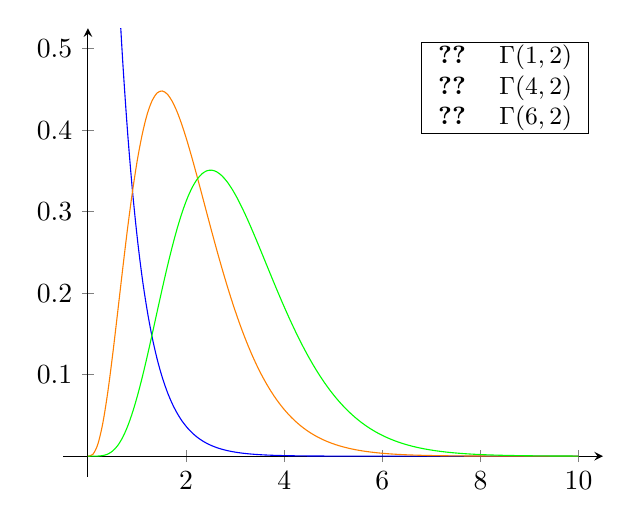
\begin{tikzpicture}
		\begin{axis}[
			name=GammaDistribution,
			axis y line=middle,
			axis x line=middle,
			enlarge x limits=0.05,
			enlarge y limits=0.05,
			ymax=.5,
			ymin=0,
		]
			\def\plotGDPDF#1#2#3{\addplot[color=#3,samples=100,smooth,domain=0:10]{%定义
				(2^(#1))*(x^(#1-1))*exp(-2*x)/(#2)
			}}%
			\plotGDPDF{1}{1}{blue};\label{pgfplots:伽马分布.Gamma(1,2)}
			\plotGDPDF{4}{6}{orange};\label{pgfplots:伽马分布.Gamma(4,2)}
			\plotGDPDF{6}{120}{green};\label{pgfplots:伽马分布.Gamma(6,2)}
		\end{axis}
		\node[draw,fill=white,inner sep=0pt,below left=0.5em]
		at(GammaDistribution.north east){\small\begin{tabular}{cl}
			\ref{pgfplots:伽马分布.Gamma(1,2)} & \(\Gamma(1,2)\) \\
			\ref{pgfplots:伽马分布.Gamma(4,2)} & \(\Gamma(4,2)\) \\
			\ref{pgfplots:伽马分布.Gamma(6,2)} & \(\Gamma(6,2)\) \\
		\end{tabular}};
	\end{tikzpicture}
	\caption{\(\Gamma\)分布的密度函数}
	% Mathematica: Plot[Table[PDF[GammaDistribution[\[Alpha], .5], x], {\[Alpha], {1, 4, 6}}] // Evaluate, {x, 0, 20}, PlotRange -> {0, .5}, Filling -> Axis]
\end{figure}


\begin{definition}
若一个元件或系统的寿命\(X\)满足一个连续型分布,\(X \sim F(t)\),
则其可靠度函数定义为\[
R(t) = 1 - F(t) = P(X > t).
\]其失效率函数定义为\[
r(t) = \frac{f(t)}{R(t)}.
\]

当\(\increment t\)较小时,\(r(t) \increment t\)表示元件或系统在时刻\(t\)以前正常工作,
但在时间\((t,t+\increment t)\)失效的概率.
\end{definition}

注意,当\(\alpha = 1\)时,\(\Gamma\)分布\(\Gamma(1,\beta)\)为指数分布\(e(\beta)\),即系统失效概率不随时间变化;
当\(0 < \alpha < 1\)时,系统失效概率随时间\(t\)增加呈下降趋势;而当\(\alpha > 1\)时则正相反.

\subsubsection{贝塔分布}
\begin{definition}
%@see: 《概率论与数理统计》(茆诗松、周纪芗、张日权) P90.
若随机变量\(X\)有密度函数\begin{equation}
	f(x) = \frac{1}{B(\alpha,\beta)} x^{\alpha-1} (1-x)^{\beta-1},
	\quad 0\leq x\leq1,
\end{equation}
其中\(\alpha,\beta\)是正常数,
\(B\)是\hyperref[equation:特殊函数.贝塔函数的定义式]{贝塔函数},
则称“\(X\)服从~\DefineConcept{\(B\)分布}”,
记为\(X \sim B(\alpha,\beta)\).
%@see: https://mathworld.wolfram.com/BetaDistribution.html
\end{definition}

\section{随机变量的函数的分布}
在实际应用中,常常遇到随机变量的函数.
如一个圆柱状工件的半径为\(X\),则工件截面积为\(\pi X^2\).
一般地,随机变量\(X\)的函数\(Y=g(X)\)是一个样本空间到实数域的复合函数,所以\(Y\)也是随机变量.
因此有依据\(X\)的分布求出\(Y\)的分布的问题.
这样的问题在离散的情形下较为简单,在连续的情形下较为复杂.

\subsection{求解离散型随机变量函数的概率分布的基本方法步骤}
设随机变量\(X\)的概率分布为\(p_k = P(X = x_k)\ (k=1,2,\dotsc)\),
则\(Y = g(X)\)的概率分布为\[
P(Y = y_j) = \sum_{g(x_k) = y_j} p_k
\quad(j=1,2,\dotsc).
\]

\begin{example}
设随机变量\(X\)的概率分布为\[
X \sim \begin{pmatrix}
-1 & 0 & 1 & 2 \\
0.2 & 0.3 & 0.3 & 0.2
\end{pmatrix},
\]\(Y=X^2\),\(Z=\frac{X^3+1}{2}\),求\(Y,Z\)的概率分布.
\begin{solution}
由于\(X\in\{-1,0,1,2\}\),所以\(Y\in\{0,1,4\}\),\begin{align*}
P(Y=0) &= P(X=0) = 0.3, \\
P(Y=1) &= P(X=-1 \lor X=1) \\
	&= P(X=-1) + P(X=1)
	= 0.5, \\
P(Y=4) &= P(X=2) = 0.2,
\end{align*}
从而\[
Y \sim \begin{pmatrix}
0 & 1 & 4 \\
0.3 & 0.5 & 0.2
\end{pmatrix}.
\]

同理,\(Z\in\Set{0,\frac{1}{2},1,\frac{9}{2}}\),且\begin{align*}
P(Z=0) &= P(X=-1) = 0.2, \\
P(Z=1/2) &= P(X=0) = 0.3, \\
P(Z=1) &= P(X=1) = 0.3, \\
P(Z=9/2) &= P(X=2) = 0.2,
\end{align*}
从而\[
Z \sim \begin{pmatrix}
0 & \frac{1}{2} & 1 & \frac{9}{2} \\
0.2 & 0.3 & 0.3 & 0.2
\end{pmatrix}.
\]
\end{solution}
\end{example}

\subsection{求解连续型随机变量函数的密度函数的基本方法步骤}
设随机变量\(X\)的密度函数为\(f_X(x)\),
要求\(Y = g(X)\)的密度函数,
\begin{enumerate}
	\item 首先依据\(X\)的取值区间,
	求出\(Y\)的值域\(R(Y)\).

	\item 然后求出\(Y\)的分布函数,
	即对\(\forall y \in R(Y)\),
	有\[
		F_Y(y) = P(Y \leq y)
		= P[g(X) \leq y]
		= P[X \in G(y)]
		= \int_{G(y)} f_X(x) \dd{x},
	\]
	其中\(G(y) = \Set{ x\in\mathbb{R} \given g(x) \leq y }\).
	对\(\forall y \notin R(Y)\),
	有\[
		F_Y(y) = 0
		\quad\text{或}\quad
		F_Y(y) = 1.
	\]

	\item 对\(Y\)的分布函数求导,得\[
		f_Y(y) = \left\{ \begin{array}{cl}
			F_Y'(y), & y \in R(Y), \\
			0, & y \notin R(Y).
		\end{array} \right.
	\]
\end{enumerate}


\chapter{多维随机变量及其分布}
\section{二维随机变量及其分布函数}
\subsection{二维随机变量及其分布函数}
\begin{definition}
%@see: 《概率论与数理统计》(陈鸿建、赵永红、翁洋) P64 定义3.1
设\(X\)与\(Y\)是定义在同一样本空间\(\Omega\)上的两个随机变量,
则称“\((X,Y)\)是\DefineConcept{二维随机变量}”
或“\((X,Y)\)是\DefineConcept{二维随机向量}”.
\end{definition}

随机变量\(X\)与\(Y\)从不同角度刻画同一随机试验,
因此需要作为一个整体研究二维随机变量\((X,Y)\)的统计规律性,
这就是\((X,Y)\)的分布函数.

\begin{definition}
%@see: 《概率论与数理统计》(陈鸿建、赵永红、翁洋) P64 定义3.2
设\((X,Y)\)是二维随机变量,
对任意实数\(x,y\),
把\begin{equation}\label{equation:多维随机变量及其分布.二维分布函数的定义式}
%@see: 《概率论与数理统计》(陈鸿建、赵永红、翁洋) P64 (3.1.1)
	F(x,y) = P(X \leq x, Y \leq y)
\end{equation}
称为“二维随机变量\((X,Y)\)的\DefineConcept{二维分布函数}”
或“\(X\)与\(Y\)的\DefineConcept{联合分布函数}(joint distribution function)”.
%@see: https://mathworld.wolfram.com/JointDistributionFunction.html
\end{definition}
二维分布函数\(F(x,y)\)表示事件\((X \leq x)\)与\((Y \leq y)\)同时发生的概率.
如果将\((X,Y)\)看为平面上的随机点坐标,
则\(F(x,y)\)为\((X,Y)\)
落在广义矩形区域\(G=\Set{(u,v) \given u \leq x, v \leq y}\)上的概率.

特别地,\((X,Y)\)落在矩形区域\((x_1,x_2]\times(y_1,y_2]\)上的概率为
\begin{equation}
%@see: 《概率论与数理统计》(陈鸿建、赵永红、翁洋) P64 (3.1.2)
	P(x_1 < X \leq x_2, y_1 < Y \leq y_2)
	= F(x_2,y_2) - F(x_2,y_1) - F(x_1,y_2) + F(x_1,y_1).
\end{equation}

与一维随机变量的分布函数类似,二维分布函数\(F(x,y)\)具有如下性质:
\begin{property}
%@see: 《概率论与数理统计》(陈鸿建、赵永红、翁洋) P64 定理3.1
设\(F(x,y)\)为随机变量\((X,Y)\)的分布函数,则
\begin{enumerate}
	\item \(F(x,y)\)分别关于\(x\)及\(y\)单调不减,即
	当\(x_1 < x_2\)时,有\(F(x_1,y) \leq F(x_2,y)\);
	当\(y_1 < y_2\)时,有\(F(x,y_1) \leq F(x,y_2)\).

	\item \(F(-\infty,-\infty)=F(-\infty,y)=F(x,-\infty)=0\),
	\(F(+\infty,+\infty)=1\).

	\item \(F(x,y)\)关于\(x\)及\(y\)都右连续,
	即对任意实数\(x\)、\(y\)有
	\(F(x^+,y)=F(x,y)\)和\(F(x,y^+)=F(x,y)\)成立.

	\item 对任意\(x_1 < x_2\)、\(y_1 < y_2\)有\[
		P(x_1 < X \leq x_2, y_1 < Y \leq y_2)
		= F(x_2,y_2) - F(x_2,y_1) - F(x_1,y_2) + F(x_1,y_1)
		\geq 0.
	\]
\end{enumerate}
\end{property}

需要指出,上述四点也是二维分布函数的特征,也就是说,
任何一个二元函数只要满足这四点就是某二维随机变量的分布函数.

\begin{example}
%@see: 《概率论与数理统计》(陈鸿建、赵永红、翁洋) P65 例3.1
考虑二元函数\[
	G(x,y) = \left\{ \begin{array}{cl}
		1, & x+y\geq0, \\
		0, & x+y<0.
	\end{array} \right.
\]
由于\[
	G(1,1)-G(1,-0.5)-G(-0.5,1)+G(-0.5,-0.5)=-1,
\]
所以\(G\)不是二维分布函数.
\end{example}

\subsection{二维离散型随机变量及其概率分布的概念与性质}
\begin{definition}
%@see: 《概率论与数理统计》(陈鸿建、赵永红、翁洋) P65
如果二维随机变量\((X,Y)\)只取有限个或可数无穷个点对\((x_i,y_i)\ (i,j=1,2,\dotsc)\),
则称\((X,Y)\)为\DefineConcept{二维离散型随机变量}.
\end{definition}

\begin{definition}
%@see: 《概率论与数理统计》(陈鸿建、赵永红、翁洋) P65 定义3.3
设二维离散型随机变量\((X,Y)\)所有可能取值为\((x_i,y_i)\ (i,j=1,2,\dotsc)\).
把\[
	p_{ij} = P(X = x_i, Y = y_j)
	\quad(i,j = 1,2,\dotsc)
\]称为“\((X,Y)\)的\DefineConcept{二维概率分布}”,
“\((X,Y)\)的\DefineConcept{二维分布律}”,
或“\(X\)与\(Y\)的\DefineConcept{联合概率分布}”.
\end{definition}

二维概率分布可以用\cref{table:多维随机变量及其分布.二维概率分布} 表示.

\begin{table}[htb]
	\centering
	\begin{tblr}{c|*5c}
		\diagbox{$X$}{$Y$}
			& \(y_1\) & \(y_2\) & \(\dots\) & \(y_j\) & \(\dots\) \\ \hline
		\(x_1\) & \(p_{11}\) & \(p_{12}\) & \(\dots\) & \(p_{1j}\) & \(\dotsc\) \\
		\(x_2\) & \(p_{21}\) & \(p_{22}\) & \(\dots\) & \(p_{2j}\) & \(\dotsc\) \\
		\(\vdots\) & \(\vdots\) & \(\vdots\) & & \(\vdots\) \\
		\(x_i\) & \(p_{i1}\) & \(p_{i2}\) & \(\dots\) & \(p_{ij}\) & \(\dotsc\) \\
		\(\vdots\) & \(\vdots\) & \(\vdots\) & & \(\vdots\) \\
	\end{tblr}
	\caption{\((X,Y)\)的二维概率分布}
	\label{table:多维随机变量及其分布.二维概率分布}
\end{table}

\begin{property}
%@see: 《概率论与数理统计》(陈鸿建、赵永红、翁洋) P66
二维离散型随机变量的概率分布有如下的性质:
\begin{enumerate}
	\item {\rm\bf 非负性}:
	\(p_{ij} \geq 0\ (i,j=1,2,\dotsc)\);

	\item {\rm\bf 规范性}:
	\(\sum_{i,j} p_{ij} = 1\).
\end{enumerate}
\end{property}

\begin{theorem}
对于任意一个二维点集\(G\),
对任意二维离散型随机变量\((X,Y)\)可以求事件\(((X,Y) \in G)\)的概率,
即\[
%@see: 《概率论与数理统计》(陈鸿建、赵永红、翁洋) P66 (3.1.4)
	P\left[(X,Y) \in G\right] = \sum_{(x_i,y_j) \in G} p_{ij}.
\]

特别地,二维离散型随机变量\((X,Y)\)的二维分布函数可用概率分布求出,即\[
%@see: 《概率论与数理统计》(陈鸿建、赵永红、翁洋) P66 (3.1.5)
	F(x,y) = \sum_{x_i \leq x}\sum_{y_j \leq y} p_{ij},
\]且有\[
%@see: 《概率论与数理统计》(陈鸿建、赵永红、翁洋) P66 (3.1.6)
	p_{ij} = F(x_i,y_j) - F(x_i,y_{j-1}) - F(x_{i-1},y_j) + F(x_{i-1},y_{j-1}),
	\quad i,j = 1,2,\dotsc,
\]
其中,规定\(x_0 = y_0 = -\infty\).
\end{theorem}

\subsection{常见的二维离散型分布}
\subsubsection{三项分布}
\begin{definition}
%@see: 《概率论与数理统计》(陈鸿建、赵永红、翁洋) P67
在\(n\)重独立试验中,若每次试验只有\(A_1\)、\(A_2\)、\(A_3\)三个可能结果,
且\(0 < p_i = P(A_i) < 1\ (i=1,2,3)\),则\(p_1 + p_2 + p_3 = 1\).
令随机变量\(X\)及\(Y\)分别表示\(n\)次试验中\(A_1\)与\(A_2\)发生的次数,
则\(X\)与\(Y\)的联合概率分布为\[
%@see: 《概率论与数理统计》(陈鸿建、赵永红、翁洋) P67 (3.1.7)
	P(X=k_1,Y=k_2)
	= \frac{n!}{k_1! k_2! (n-k_1-k_2)!} p_1^{k_1} p_2^{k_2} p_3^{n-k_1-k_2},
\]
其中\(k_1+k_2 = 0,1,\dotsc,n\),\(k_1 \geq 0\),\(k_2 \geq 0\),
并称“\((X,Y)\)服从参数为\(p _1,p_2,n\)的\DefineConcept{三项分布}”,
记为\((X,Y) \sim T(n;p_1,p_2)\).
\end{definition}

\subsection{二维连续型随机变量及其密度函数的概念与性质}
\begin{definition}
%@see: 《概率论与数理统计》(陈鸿建、赵永红、翁洋) P68 定义3.4
设二维随机变量\((X,Y)\)有分布函数\(F(x,y)\),
如果存在二元非负函数\(f(x,y)\),
使得对任意实数\(x,y\)有\[
%@see: 《概率论与数理统计》(陈鸿建、赵永红、翁洋) P68 (3.1.8)
	F(x,y) = \int_{-\infty}^x \int_{-\infty}^y f(u,v) \dd{u} \dd{v},
\]
则称“\((X,Y)\)是\DefineConcept{二维连续型随机变量}”,
称“\(f(x,y)\)是\((X,Y)\)的\DefineConcept{二维概率密度函数}”,
或“\(f(x,y)\)是\(X\)与\(Y\)的\DefineConcept{联合密度函数}”.
\end{definition}

\begin{property}
%@see: 《概率论与数理统计》(陈鸿建、赵永红、翁洋) P68
二维连续型随机变量的密度函数有如下的性质:
\begin{enumerate}
	\item {\rm\bf 非负性}:
	\((\forall (x,y)\in\mathbb{R}^2)[f(x,y) \geq 0]\);

	\item {\rm\bf 规范性}:
	\(F(+\infty,+\infty)
	= \int_{-\infty}^{+\infty} \int_{-\infty}^{+\infty} f(x,y) \dd{x} \dd{y} = 1\).
\end{enumerate}
\end{property}

\begin{theorem}
%@see: 《概率论与数理统计》(陈鸿建、赵永红、翁洋) P68 定理3.2
设二维连续型随机变量\((X,Y)\)有密度函数\(f(x,y)\),则
\begin{enumerate}
	\item \(F(x,y)\)是连续函数且在\(f(x,y)\)的连续点\((x,y)\),
	有\[
	%@see: 《概率论与数理统计》(陈鸿建、赵永红、翁洋) P68 (3.1.10)
		f(x,y) = \pdv{F(x,y)}{x}{y};
	\]

	\item 对平面上任意区域\(G \subseteq \mathbb{R}^2\),
	若\(f(x,y)\)在\(G\)上可积,
	有\[
	%@see: 《概率论与数理统计》(陈鸿建、赵永红、翁洋) P68 (3.1.11)
		P\left[(X,Y) \in G\right] = \iint_G{f(x,y) \dd{x}\dd{y}};
	\]

	\item 对平面上任一条曲线\(L\),有\[
		P\left[(X,Y) \in L\right] = 0.
	\]
\end{enumerate}
\end{theorem}

\subsection{常见的二维连续型分布}
\subsubsection{均匀分布}
\begin{definition}
令\(G\)是平面上一个有界区域,若二维随机变量\((X,Y)\)有密度函数\[
%@see: 《概率论与数理统计》(陈鸿建、赵永红、翁洋) P68 (3.1.12)
	f(x,y) = \left\{ \begin{array}{ll}
		\frac{1}{m(G)}, & (x,y) \in G, \\
		0, & \text{其他}, \\
	\end{array} \right.
\]
其中\(m(G)\)为\(G\)的面积,
则称“\((X,Y)\)服从在\(G\)上的\DefineConcept{均匀分布}”,
记为\((X,Y) \sim U(G)\).
\end{definition}

\subsubsection{二维正态分布}
\begin{definition}
%@see: 《概率论与数理统计》(陈鸿建、赵永红、翁洋) P145 定义5.3
设二维随机变量\((X,Y)\)有二维密度函数
\begin{equation}
	f(x,y) = \frac{1}{2\pi\sigma_1\sigma_2\sqrt{1-r^2}}
		\exp\left[- u\left(
			\frac{x-\mu_1}{\sigma_1},
			\frac{y-\mu_2}{\sigma_2}
		\right)\right]
	\quad(x,y)\in\mathbb{R}^2,
\end{equation}
其中\[
	u(x,y)
	= \frac{1}{2(1-r^2)}
	\begin{bmatrix}
		x & y
	\end{bmatrix}
	\begin{bmatrix}
		1 & -r \\
		-r & 1
	\end{bmatrix}
	\begin{bmatrix}
		x \\ y
	\end{bmatrix},
\]
\(\mu_1\in\mathbb{R},
\mu_2\in\mathbb{R},
\sigma_1\in\mathbb{R}^+,
\sigma_2\in\mathbb{R}^+,
r\in(-1,1)\)是参数,
则称“\((X,Y)\)服从\DefineConcept{二维正态分布}”,
记为\((X,Y) \sim N(\mu_1,\mu_2;\sigma_1^2,\sigma_2^2;r)\).
\end{definition}

\begin{theorem}\label{theorem:正态分布与自然指数分布族.性质1}
%@see: 《概率论与数理统计》(陈鸿建、赵永红、翁洋) P145 定理5.6
若\((X,Y) \sim N(\mu_1,\mu_2;\sigma_1^2,\sigma_2^2;r)\),
则对应的边缘分布均为正态分布,且\[
	X \sim N(\mu_1,\sigma_1^2),
	\qquad
	Y \sim N(\mu_2,\sigma_2^2).
\]
\begin{proof}
首先有\begin{align*}
	f_X(x) = \int_{-\infty}^{+\infty} f(x,y) \dd{y}
	= \frac{1}{2\pi\sigma_1\sigma_2\sqrt{1-r^2}}
		\int_{-\infty}^{+\infty} e^{-u(x,y)} \dd{y},
\end{align*}
其中\begin{align*}
	u(x,y)
	&= \frac{1}{2(1-r^2)} \left[
			\frac{(x-\mu_1)^2}{\sigma_1^2}
			-2r\frac{(x-\mu_1)(y-\mu_2)}{\sigma_1\sigma_2}
			+\frac{(y-\mu_2)^2}{\sigma_2^2}
		\right] \\
	&= \frac{1}{2 \sigma_1^2} (x-\mu_1)^2
		+ \frac{1}{2(1-r^2)} \left[
			\frac{y-\mu_2}{\sigma_2}
			- \frac{r(x-\mu_1)^2}{\sigma_1}
		\right]^2.
\end{align*}
令\[
	t = \frac{1}{\sqrt{1-r^2}} \left[
		\frac{y-\mu_2}{\sigma_2}
		- \frac{r(x-\mu_1)}{\sigma_1}
	\right],
\]
则有\[
	f_X(x)
	= \frac{1}{\sqrt{2\pi} \sigma_1} e^{-\frac{(x-\mu_1)^2}{2\sigma_1^2}} \int_{-\infty}^{+\infty} \frac{1}{\sqrt{2\pi}} e^{-\frac{t^2}{2}} \dd{t} \\
	= \frac{1}{\sqrt{2\pi} \sigma_1} e^{-\frac{(x-\mu_1)^2}{2\sigma_1^2}}
	\quad(x\in\mathbb{R}).
\]
同理可得\[
	f_Y(y)
	= \frac{1}{\sqrt{2\pi} \sigma_2} e^{-\frac{(y-\mu_2)^2}{2\sigma_2^2}}
	\quad(y\in\mathbb{R}).
	\qedhere
\]
\end{proof}
\end{theorem}

二维正态分布的条件分布仍然是正态分布.
\begin{example}\label{theorem:正态分布与自然指数分布族.性质4}
%@see: 《概率论与数理统计》(陈鸿建、赵永红、翁洋) P147 例5.7
设二维随机变量\((X,Y) \sim N(\mu_1,\mu_2;\sigma_1^2,\sigma_2^2;r)\).
求条件密度\(f_{X \vert Y}(x \vert y)\).
\begin{solution}
\def\A{\frac{1}{\sqrt{2\pi}\sigma_1\sqrt{1-r^2}}}%
\def\B{\frac{1}{2(1-r^2)}}%
直接计算得\begin{align*}
	&f_{X \vert Y}(x \vert y) = \frac{f(x,y)}{f_Y(y)} \\
	&= \A
		\exp\Biggl\{
			- \B
			\left[
				\frac{(x-\mu_1)^2}{\sigma_1^2}
				- 2r\frac{(x-\mu_1)(y-\mu_2)}{\sigma_1\sigma_2}
				+ r^2\frac{(y-\mu_2)^2}{\sigma_2^2}
			\right]
		\Biggr\} \\
	&= \A
		\exp\left\{
			- \B
			\left[
				\frac{x-\mu_1}{\sigma_1}
				- r\frac{y-\mu_2}{\sigma_2}
			\right]^2
		\right\} \\
	&= \A
		\exp\left\{
			- \B
			\frac{1}{\sigma_1^2}
			\left[
				x - \mu_1
				- r\frac{\sigma_1}{\sigma_2}(y-\mu_2)
			\right]^2
		\right\}.
\end{align*}
这个条件密度函数恰好是期望为\(\mu_1+r\frac{\sigma_1}{\sigma_2}(y-\mu_2)\),
方差为\(\sigma_1^2(1-r^2)\)的正态分布的密度函数.
\end{solution}
\end{example}

\begin{theorem}\label{theorem:正态分布与自然指数分布族.二维随机变量服从二维正态分布的充分必要条件}
%@see: 《概率论与数理统计》(陈鸿建、赵永红、翁洋) P147 定理5.8
二维随机变量\((X,Y)\)服从二维正态分布的充分必要条件是:
\(X\)与\(Y\)的任意非零线性组合\(Z=aX+bY\)服从一维正态分布,
即\(Z \sim N(E(Z),D(Z))\).
\end{theorem}

\begin{example}
%@see: 《概率论与数理统计》(陈鸿建、赵永红、翁洋) P147 例5.8
设\((X,Y) \sim N\left(2,3;4,9;\frac{1}{2}\right)\),
\(Z = \frac{1}{2} X - \frac{1}{3} Y\),
求\(E(\abs{Z})\).
\begin{solution}
由\cref{theorem:正态分布与自然指数分布族.性质1} 有\[
	X \sim N(2,4), \qquad
	Y \sim N(3,9),
\]且相关系数\(R(X,Y) = 1/2\),
于是\[
	\Cov(X,Y) = R(X,Y) \sqrt{D(X)} \sqrt{D(Y)} = 3.
\]\[
	E(Z) = \frac{1}{2} E(X) - \frac{1}{3} E(Y) = 0.
\]\[
	D(Z) = \frac{1}{4} D(X) + \frac{1}{9} D(Y)
		- 2 \cdot \frac{1}{2} \cdot \frac{1}{3} \Cov(X,Y)
	= 1.
\]
由\cref{theorem:正态分布与自然指数分布族.二维随机变量服从二维正态分布的充分必要条件}
有\begin{align*}
	E(\abs{Z})
	&= \int_{-\infty}^{+\infty} \abs{z} \frac{1}{\sqrt{2\pi}} e^{-\frac{z^2}{2}} \dd{z}
	= \frac{2}{\sqrt{2\pi}} \int_0^{+\infty} z e^{-\frac{z^2}{2}} \dd{z} \\
	&= \frac{\sqrt{2}}{\sqrt{\pi}} \int_0^{+\infty} \dd(-e^{-\frac{z^2}{2}})
	= \sqrt{\frac{2}{\pi}} \left(-e^{-\frac{z^2}{2}}\right)_0^{+\infty}
	= \sqrt{\frac{2}{\pi}}.
\end{align*}
\end{solution}
\end{example}

\begin{example}
设随机变量\(X\)、\(Y\)相互独立,且\(X \sim U(0,1)\),\(Y \sim e(1/2)\).
求关于\(a\)的一元二次方程\(a^2 + 2aX + Y = 0\)有实根的概率.
\begin{solution}
根据均匀分布和指数分布的定义,\[
	f_X(x) = \left\{ \begin{array}{cl}
		1, & x\in(0,1), \\
		0, & \text{其他};
	\end{array} \right.
	\qquad
	f_Y(y) = \left\{ \begin{array}{cl}
		\frac{1}{2} e^{-\frac{1}{2} y}, & y>0, \\
		0, & y \leq 0.
	\end{array} \right.
\]
因为随机变量\(X\)、\(Y\)相互独立,
所以\(X\)与\(Y\)的联合密度函数为\[
	f(x,y) = f_X(x) \cdot f_Y(y)
	= \left\{ \begin{array}{cl}
		\frac{1}{2} e^{-\frac{1}{2} y}, & 0<x<1 \land y>0, \\
		0, & \text{其他}.
	\end{array} \right.
\]

一元二次方程有实根的概率为\begin{align*}
	P[(2X)^2 - 4Y \geq 0]
	&= P(X^2 \geq Y)
	= \int_0^1 \dd{x} \int_0^{x^2} \frac{1}{2} e^{-\frac{1}{2} y} \dd{y} \\
	&= 1 - \sqrt{2\pi} \left[ \Phi(1) - \frac{1}{2} \right]
	\approx 0.144~376.
\end{align*}
\end{solution}
\end{example}

\begin{example}
设二维随机变量\((X,Y)\)的概率密度为\[
	f(x,y) = A e^{-2x^2+2xy-y^2}, \quad x,y\in\mathbb{R},
\]
求常数\(A\)及条件概率密度\(f_{Y \vert X}(y \vert x)\).
\begin{solution}
先求\(X\)的边缘密度函数,有\begin{align*}
	f_X(x) &= \int_{-\infty}^{+\infty} f(x,y) \dd{y} \\
	&= \int_{-\infty}^{+\infty} A e^{-2x^2+2xy-y^2} \dd{y} \\
	&= A e^{-x^2} \int_{-\infty}^{+\infty} e^{-(y-x)^2} \dd{y} \\
	&= A e^{-x^2} \sqrt{\pi} \int_{-\infty}^{+\infty}
		\frac{1}{\sqrt{2\pi} \sqrt{\frac{1}{2}}}
		e^{\frac{-(y-x)^2}{2 \cdot \frac{1}{2}}} \dd{y} \\
	&= A \sqrt{\pi} e^{-x^2}.
\end{align*}
由\hyperref[theorem:随机变量及其分布.连续型随机变量的密度函数的性质]{规范性}%
和重要积分公式 \labelcref{equation:重积分.常用积分2} 可知\[
	\int_{-\infty}^{+\infty} f_X(x) \dd{x}
	= A \sqrt{\pi} \int_{-\infty}^{+\infty} e^{-x^2} \dd{x}
	= A \pi = 1,
\]
因此,\(A = \frac{1}{\pi}\).
那么根据\cref{equation:多维随机变量及其分布.条件密度、联合密度、边缘密度的关系2} 有\[
	f_{Y \vert X}(y \vert x)
	= \frac{f(x,y)}{f_X(x)}
	= \frac{\frac{1}{\pi} e^{-2x^2+2xy-y^2}}{\frac{1}{\pi} \sqrt{\pi} e^{-x^2}}
	= \frac{1}{\sqrt{\pi}} e^{-(x-y)^2},
	\quad y\in\mathbb{R}.
\]
\end{solution}
\end{example}

\section{边缘分布及随机变量的独立性}
\subsection{边缘分布函数与随机变量的独立性}
\begin{definition}
二维随机变量\((X,Y)\)的分量\(X\)、\(Y\)均可看作一维随机变量.
这两个分量各自的分布函数\(F_X(x)\)、\(F_Y(y)\),
相对于二维分布函数\(F(x,y)\)而被分别称为\(X\)与\(Y\)的\DefineConcept{边缘分布函数}.
\end{definition}

\begin{theorem}
设\(F(x,y)\)为二维随机变量\((X,Y)\)的二维分布函数,
则\(X\)与\(Y\)的边缘分布函数\(F_X(x)\)、\(F_Y(y)\)有
\begin{align*}
	F_X(x) &= F(x,+\infty), \quad x \in \mathbb{R}; \\
	F_Y(y) &= F(+\infty,y), \quad y \in \mathbb{R}.
\end{align*}
\end{theorem}

\begin{definition}
%@see: 《概率论与数理统计》(茆诗松、周纪芗、张日权) P132 定义3.2.1
设\(\AutoTuple{X}{n}\)是\(n\)维随机变量.
若对任意\(n\)个实数\(\AutoTuple{x}{n}\),
\(n\)个事件\((X_1 \leq x_1),\dotsc,(X_n \leq x_n)\)相互独立,
即有\[
	P(X_1 \leq x_1,\dotsc,X_n \leq x_n)
	= P(X_1 \leq x_1) \dotsm P(X_n \leq x_n)
\]
或\[
	F(x_1,\dotsc,x_n)
	= F_1(x_1) \dotsm F_n(x_n),
\]
其中\(F\)是\(n\)维随机变量\(\AutoTuple{X}{n}\)的联合分布函数,
而\(F_1,\dotsc,F_n\)分别是\(X_1,\dotsc,X_n\)的边缘分布函数,
则称“\(n\)个随机变量\(\AutoTuple{X}{n}\)~\DefineConcept{相互独立}”;
否则称“\(n\)个随机变量\(\AutoTuple{X}{n}\)~\DefineConcept{不相互独立}”
或“\(n\)个随机变量\(\AutoTuple{X}{n}\)~\DefineConcept{相依}”.
\end{definition}

\begin{theorem}
设随机变量\(X\)与\(Y\)相互独立,且\(g(x)\)与\(h(y)\)均是连续函数,
则\(X_1 = g(X)\)与\(Y_1 = h(Y)\)也相互独立.
\end{theorem}

\subsection{二维离散型随机变量的边缘分布及独立性}
\begin{definition}
设\((X,Y)\)是二维离散型随机变量,有二维概率分布\[
p_{ij} = P(X=x_i,Y=y_j), \quad i,j=1,2,\dotsc.
\]显然此时\(X\)与\(Y\)都是一维离散型随机变量,各有分布律
\begin{align*}
p_{i*} &= P(X=x_i), \quad i=1,2,\dotsc; \\
p_{*j} &= P(Y=y_j), \quad j=1,2,\dotsc.
\end{align*}
相对于二维概率分布,\(X\)与\(Y\)各自的分布叫做\DefineConcept{边缘概率分布},简称\DefineConcept{边缘分布}.
\end{definition}

\begin{theorem}
设\((X,Y)\)是二维离散型随机变量,有二维概率分布\[
p_{ij} = P(X=x_i,Y=y_j), \quad i,j=1,2,\dotsc.
\]分量\(X\)与\(Y\)的边缘分布可由二维概率分布求出,即
\begin{align*}
p_{i*} = \sum_{j}{p_{ij}}, \quad i=1,2,\dotsc; \\
p_{*j} = \sum_{i}{p_{ij}}, \quad j=1,2,\dotsc.
\end{align*}
\end{theorem}

\begin{theorem}
设\((X,Y)\)是二维离散型随机变量,有二维概率分布\[
p_{ij} = P(X=x_i,Y=y_j), \quad i,j=1,2,\dotsc,
\]则随机变量\(X\)与\(Y\)相互独立的充分必要条件是:\[
p_{ij} = p_{i*} p_{*j}, \quad i,j=1,2,\dotsc.
\]
\end{theorem}

\subsection{二维连续型随机变量的边缘密度及独立性}
\begin{theorem}
设二维连续型随机变量\((X,Y)\)的二维密度为\(f(x,y)\),
\(X\)与\(Y\)的边缘密度分别为\(f_X(x)\)和\(f_Y(y)\),则
\begin{align*}
	f_X(x) = \int_{-\infty}^{+\infty} f(x,y) \dd{y}, \\
	f_Y(y) = \int_{-\infty}^{+\infty} f(x,y) \dd{x}.
\end{align*}

而\(X\)与\(Y\)相互独立的充分必要条件是:\[
	f(x,y) = f_X(x) f_Y(y).
\]在三个密度函数的公共连续点上成立.
\end{theorem}

\section{条件分布与条件密度}
当二维随机变量\((X,Y)\)中\(X\)与\(Y\)不独立时,
随机变量\(X\)与\(Y\)应有一定的相互影响的关系,
即当\(P(Y = y) > 0\)时,
通常有\(P(X \leq x \vert Y = y) \neq P(X \leq x)\).
可以看出,条件概率\(P(X \leq x \vert Y = y)\)一般受\(y\)的影响.
于是我们把\[
	F_{X \vert Y}(x \vert y)
	\defeq
	P(X \leq x \vert Y = y)
	\quad(x\in\mathbb{R})
\]称为“\(Y=y\)条件下\(X\)的\DefineConcept{条件分布函数}”.

\subsection{离散型随机变量的条件分布}
设二维离散型随机变量\((X,Y)\)有二维概率分布\[
	p_{ij} = P(X=x_i,Y=y_j),
	\quad i,j=1,2,\dotsc.
\]
从而\(X\)及\(Y\)有边缘分布\begin{align*}
	p_{i*}
	&= P(X=x_i)
	= \sum_j p_{ij},
	\quad i=1,2,\dotsc; \\
	p_{*j}
	&= P(Y=y_j)
	= \sum_i p_{ij},
	\quad j=1,2,\dotsc.
\end{align*}
那么,对于任意给定\(y_j\),
若\(P(Y=y_j) = p_{*j} > 0\),
称\[
	P(X=x_i \vert Y=y_j) = \frac{p_{ij}}{p_{*j}}, \quad i=1,2,\dotsc
\]为\(Y=y_j\)条件下\(X\)的\DefineConcept{条件概率分布}.
同理,对于任意给定\(x_i\),
若\(P(X=x_i) = p_{i*} > 0\),
称\[
	P(Y=y_j \vert X=x_i) = \frac{p_{ij}}{p_{i*}}, \quad j=1,2,\dotsc
\]为\(X=x_i\)条件下\(Y\)的\DefineConcept{条件概率分布}.

\begin{property}
离散型随机变量的条件概率分布有如下性质:
\begin{enumerate}
	\item \(P(X=x_i \vert Y=y_j) \geq 0, \quad i=1,2,\dotsc;\)
	\item \(\sum_{i}{P(X=x_i \vert Y=y_j)} = \sum_{i}{\frac{p_{ij}}{p_{*j}}} = 1.\)
\end{enumerate}
可见,条件概率分布也是离散型概率分布.
\end{property}

\begin{theorem}
对任意\(x\)、\(y\),由条件分布可得条件分布函数的表示:
\begin{align*}
	F_{X \vert Y}(x \vert y_j)
	= P(X \leq x \vert Y=y_j)
	= \sum_{x_i \leq x}{\frac{p_{ij}}{p_{*j}}}, \\
	F_{Y \vert X}(y \vert x_i)
	= P(Y \leq y \vert X=x_i)
	= \sum_{y_j \leq y}{\frac{p_{ij}}{p_{i*}}}.
\end{align*}
\end{theorem}

\subsection{连续型随机变量的条件密度函数}
\begin{definition}
设\((X,Y)\)为二维连续型随机变量.若对任意\(\epsilon > 0\),有\[
	P(y - \epsilon < Y \leq y + \epsilon) > 0,
\]
且对\(x\in\mathbb{R}\),
极限\[
	\lim_{\epsilon\to0^+} P(X \leq x \vert y - \epsilon < Y \leq y + \epsilon)
\]存在,
则称该极限为“连续型随机变量\(Y=y\)条件下\(X\)的\DefineConcept{条件分布函数}”,
记为\[
	F_{X \vert Y}(x \vert y)
	\quad\text{或}\quad
	P(X \leq x \vert Y = y).
\]

类似地,可以定义“连续型随机变量\(X=x\)条件下\(Y\)的\DefineConcept{条件分布函数}”,
记为\[
	F_{Y \vert X}(y \vert x)
	\quad\text{或}\quad
	P(Y \leq y \vert X = x).
\]
\end{definition}

\begin{theorem}
设二维连续型随机变量\((X,Y)\)有二维密度\(f(x,y)\),
从而\(X\)及\(Y\)有边缘密度\(f_X(x)\)、\(f_Y(y)\),则
\begin{align*}
	F_{X \vert Y}(x \vert y)
	= \int_{-\infty}^x \frac{f(u,y)}{f_Y(y)}\dd{u}, \quad x \in \mathbb{R}; \\
	F_{Y \vert X}(y \vert x)
	= \int_{-\infty}^y \frac{f(x,v)}{f_X(x)}\dd{v}, \quad y \in \mathbb{R}.
\end{align*}

那么,相应的密度函数
\begin{gather}
	f_{X \vert Y}(x \vert y)
	= \frac{f(x,y)}{f_Y(y)},
		\label{equation:多维随机变量及其分布.条件密度、联合密度、边缘密度的关系1} \\
	f_{Y \vert X}(y \vert x)
	= \frac{f(x,y)}{f_X(x)},
		\label{equation:多维随机变量及其分布.条件密度、联合密度、边缘密度的关系2}
\end{gather}
分别称为“\(X\)关于\(Y\)的\DefineConcept{条件密度函数}”%
和“\(Y\)关于\(X\)的\DefineConcept{条件密度函数}”.
\begin{proof}
不妨设\(f(x,y)\)连续,\(f_Y(y)\)连续且\(f_Y(y)>0\),
\def\l{\lim_{\epsilon\to0^+}}%
那么\begin{align*}
	F_{X \vert Y}(x \vert y)
	&= \lim_{\epsilon\to0^+}
		P(X \leq x \vert y - \epsilon < Y \leq y + \epsilon) \\
	&= \lim_{\epsilon\to0^+}
		\frac{
			P(X \leq x, y - \epsilon < Y \leq y + \epsilon)
		}{
			P(y - \epsilon < Y \leq y + \epsilon)
		} \\
	&= \lim_{\epsilon\to0^+}
		\frac{
			F(x,y+\epsilon) - F(x,y-\epsilon)
		}{
			F_Y(y+\epsilon) - F_Y(y-\epsilon)
		} \\
	&= \lim_{\epsilon\to0^+}
		\frac{
			[F(x,y+\epsilon) - F(x,y-\epsilon)] \frac{1}{2 \epsilon}
		}{
			[F_Y(y+\epsilon) - F_Y(y-\epsilon)] \frac{1}{2 \epsilon}
		} \\
	&= \pdv{F(x,y)}{y} \bigg/ F_Y'(y) \\
	&= \int_{-\infty}^x \frac{f(u,y)}{f_Y(y)} \dd{u}.
	\qedhere
\end{align*}
\end{proof}
\end{theorem}

可以证明,条件分布函数也是分布函数.

\begin{corollary}
已知边缘密度函数和条件密度函数,可以求出二维密度,即\[
	f(x,y) = f_Y(y) \cdot f_{X \vert Y}(x \vert y)
	= f_X(x) \cdot f_{Y \vert X}(y \vert x).
\]
\end{corollary}

\begin{example}
设\(X \sim U(0,1)\);
对\(\forall x\in(0,1)\),
当\(X=x\)时,\(Y \sim U(x^2,1)\).
求\(P(X > Y)\).
\begin{solution}
\(X\)的密度函数为\[
	f_X(x) = \left\{ \begin{array}{cl}
		1, & 0<x<1, \\
		0, & \text{其他}.
	\end{array} \right.
\]当\(X=x\in(0,1)\)时,\(Y\)有条件密度\[
	f_{Y \vert X}(y \vert x)
	= \left\{ \begin{array}{cl}
		\frac{1}{1-x^2}, & x^2<y<1, \\
		0, & \text{其他}.
	\end{array} \right.
\]因此\[
	f(x,y) = f_X(x) \cdot f_{Y \vert X}(y \vert x)
	= \left\{ \begin{array}{cl}
		\frac{1}{1-x^2}, & 0<x<1 \land x^2<y<1, \\
		0, & \text{其他}.
	\end{array} \right.
\]\[
	P(X > Y)
	= \int_0^1 \dd{x} \int_{x^2}^x \frac{1}{1-x^2} \dd{y}
	= 1 - \ln2.
\]
\end{solution}
\end{example}

\begin{example}
%@see: 《2020年全国硕士研究生入学统一考试(数学一)》三解答题/第22题
设随机变量\(X_1,X_2,X_3\)相互独立,
其中\(X_1\)与\(X_2\)均服从标准正态分布,
\(X_3\)的概率分布为\begin{equation*}
	P(X_3=0)
	= P(X_3=1)
	= \frac12.
\end{equation*}
\(Y = X_3 X_1 + (1 - X_3) X_2\).
求二维随机变量\((X_1,Y)\)的分布函数,和\(Y\)的边缘分布函数.
\begin{solution}
设\((X_1,Y)\)的分布函数为\(F(x,y)\),
则\begin{align*}
	F(x,y) &= P(X_1 \leq x,Y \leq y)
	= P(X_1 \leq x,X_3 X_1 + (1 - X_3) X_2 \leq y) \\
	% 全概率公式
	&= P(X_1 \leq x,X_3 X_1 + (1 - X_3) X_2 \leq y \vert X_3 = 0) \cdot P(X_3 = 0) \\
	&\hspace{20pt}+ P(X_1 \leq x,X_3 X_1 + (1 - X_3) X_2 \leq y \vert X_3 = 1) \cdot P(X_3 = 1) \\
	% 把条件事件代入
	&= P(X_1 \leq x,X_2 \leq y \vert X_3 = 0) \cdot P(X_3 = 0)
	+ P(X_1 \leq x,X_1 \leq y \vert X_3 = 1) \cdot P(X_3 = 1) \\
	&= P(X_1 \leq x,X_2 \leq y,X_3 = 0)
	+ P(X_1 \leq x,X_1 \leq y,X_3 = 1) \\
	&= P(X_1 \leq x) P(X_2 \leq y) P(X_3 = 0)
	+ P(X_1 \leq x,X_1 \leq y) P(X_3 = 1) \\
	&= \frac12 \Phi(x) \Phi(y) + \frac12 P(X_1 \leq \min\{x,y\}).
\end{align*}
当\(x \leq y\)时,有\begin{equation*}
	P(X_1 \leq \min\{x,y\})
	= P(X_1 \leq x) = \Phi(x).
\end{equation*}
当\(x > y\)时,有\begin{equation*}
	P(X_1 \leq \min\{x,y\})
	= P(X_1 \leq y) = \Phi(y).
\end{equation*}
因此\begin{equation*}
	F(x,y)
	= \left\{ \def\arraystretch{1.5} \begin{array}{cl}
		\frac12 \Phi(x) (\Phi(y) + 1), & x \leq y, \\
		\frac12 \Phi(y) (\Phi(x) + 1), & x > y.
	\end{array} \right.
\end{equation*}
于是\(Y\)的边缘分布为\begin{align*}
	F_Y(y) = F(+\infty,y)
	= \lim_{x\to+\infty} \frac12 \Phi(y) (\Phi(x) + 1)
	= \frac12 \Phi(y) (\Phi(+\infty) + 1)
	% \(\Phi(+\infty) = 1\)
	= \Phi(y).
\end{align*}
\end{solution}
\end{example}

\section{二维随机变量函数的分布}
\subsection{二维离散型随机变量函数的分布}
设\((X,Y)\)是二维离散型随机变量,
且\(X\)与\(Y\)有联合分布律\[
	p_{ij} = P(X=x_i,Y=y_j), \quad i,j=1,2,\dotsc,
\]
则\(Z = g(X,Y)\)有分布律\[
	P(Z=z_k) = \sum_{g(x_i,y_j)=z_k}{p_{ij}}.
\]

\begin{example}
设\((X,Y)\)有二维概率分布
\begin{center}
\begin{tikzpicture}
	\draw[thick](0,0)--(4,0) (0,-4)--+(4,0);
	\draw(0,-1)--+(4,0) (1,0)--+(0,-4);
	\draw(1.5,-.5)node{0}
		(2.5,-.5)node{1}
		(3.5,-.5)node{2}
		(.5,-1.5)node{-1}
		(.5,-2.5)node{0}
		(.5,-3.5)node{1}
		(.3,-.7)node{\(X\)}
		(.7,-.3)node{\(Y\)}
		(1.5,-1.5)node{\(\tfrac{1}{12}\)}
		(2.5,-1.5)node{\(\tfrac{2}{12}\)}
		(3.5,-1.5)node{\(\tfrac{2}{12}\)}
		(1.5,-2.5)node{\(\tfrac{1}{12}\)}
		(2.5,-2.5)node{\(\tfrac{1}{12}\)}
		(3.5,-2.5)node{\(0\)}
		(1.5,-3.5)node{\(\tfrac{2}{12}\)}
		(2.5,-3.5)node{\(\tfrac{1}{12}\)}
		(3.5,-3.5)node{\(\tfrac{2}{12}\)};
\end{tikzpicture}
\end{center}
\(Z=X+Y\),\(W=\max\{X,Y\}\),求\(Z,W\)的分布律.
\begin{solution}
我们可以根据上面的二维概率分布表格计算不同\(X,Y\)取值下\(Z\)的取值:
\begin{center}
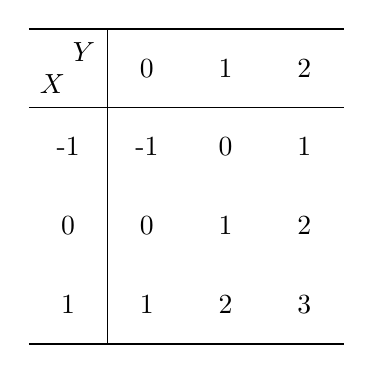
\begin{tikzpicture}
	\draw[thick](0,0)--(4,0) (0,-4)--+(4,0);
	\draw(0,-1)--+(4,0) (1,0)--+(0,-4);
	\draw(1.5,-.5)node{0}
		(2.5,-.5)node{1}
		(3.5,-.5)node{2}
		(.5,-1.5)node{-1}
		(.5,-2.5)node{0}
		(.5,-3.5)node{1}
		(.3,-.7)node{\(X\)}
		(.7,-.3)node{\(Y\)}
		(1.5,-1.5)node{-1}
		(2.5,-1.5)node{0}
		(3.5,-1.5)node{1}
		(1.5,-2.5)node{0}
		(2.5,-2.5)node{1}
		(3.5,-2.5)node{2}
		(1.5,-3.5)node{1}
		(2.5,-3.5)node{2}
		(3.5,-3.5)node{3};
\end{tikzpicture}
\end{center}
由此可知\(Z \in \Set{-1,0,1,2,3}\),那么
\def\sp#1{\sum_{x_i+y_j=#1} p_{ij}}
\begin{align*}
	&P(Z=-1) = \sp{-1} = \frac{1}{12}, \\
	&P(Z=0) = \sp{0} = \frac{1}{4}, \\
	&P(Z=1) = \sp{1} = \frac{5}{12}, \\
	&P(Z=2) = \sp{2} = \frac{1}{12}, \\
	&P(Z=3) = \sp{3} = \frac{1}{6},
\end{align*}
即\[
	Z \sim \begin{bmatrix}
		-1 & 0 & 1 & 2 & 3 \\
		\frac{1}{12} & \frac{1}{4} & \frac{5}{12} & \frac{1}{12} & \frac{1}{6}
	\end{bmatrix}.
\]
同理可得,\[
	W \sim \begin{bmatrix}
		0 & 1 & 2 \\
		\frac{1}{6} & \frac{1}{2} & \frac{1}{3}
	\end{bmatrix}.
\]
\end{solution}
\end{example}

\begin{theorem}\label{theorem:多维随机变量及其分布.离散型随机变量的卷积公式}
设二维离散型随机变量\((X,Y)\)有概率分布\(P(X=h,Y=k)\),
\(Z=X+Y\),则有\begin{align}
	P(Z=k)
	&= \sum_{r=0}^k P(X=r,Y=k-r) \\
	&= \sum_{r=0}^k P(X=k-r,Y=r).
\end{align}
特别地,当\(X\)与\(Y\)独立时,有\begin{align}
	P(Z=k)
	&= \sum_{r=0}^k P(X=r) \cdot P(Y=k-r) \label{equation:多维随机变量及其分布.离散型随机变量的卷积公式1} \\
	&= \sum_{r=0}^k P(X=k-r) \cdot P(Y=r). \label{equation:多维随机变量及其分布.离散型随机变量的卷积公式2}
\end{align}
\rm\cref{equation:多维随机变量及其分布.离散型随机变量的卷积公式1,%
equation:多维随机变量及其分布.离散型随机变量的卷积公式2}
称为“(离散型随机变量的)\DefineConcept{卷积公式}”.
\end{theorem}

\subsection{二维连续型随机变量函数的分布}
设\((X,Y)\)是二维连续型随机变量,且有密度函数\(f(x,y)\).
若\(g(x,y)\)是连续函数,
则\(Z = g(X,Y)\)是一维连续型随机变量.
\begin{enumerate}
	\item 首先写出\((X,Y)\)的联合密度函数.

	如果只知道\(X\)和\(Y\)的边缘密度函数,
	\(X\)与\(Y\)相互独立,
	则\((X,Y)\)的联合密度函数为\[
		f(x,y) = f_X(x) \cdot f_Y(y).
	\]

	如果\(Y\)是一维离散型随机变量,
	则无法写出\((X,Y)\)的联合密度函数.

	\item 根据\(X\)和\(Y\)的取值区间,确定\(Z\)的取值区间\(R(Z)\).

	\item 对任意\(z \in R(Z)\),
	求\(Z\)的分布函数\(F_Z\).

	如果我们已知\((X,Y)\)的联合密度函数\(f\),
	那么求积分可得\(Z\)的分布函数为\begin{align*}
		F_Z(z) &= P(Z \leq z)
		= P(g(X,Y) \leq z)
		= P((X,Y) \in G(z)) \\
		&= \iint_{G(z)} f(x,y) \dd{x}\dd{y}.
	\end{align*}
	这里\(G(z) = \Set{ (x,y) \given g(x,y) \leq z }\).
	当\(z \notin R(Z)\)时,有\(F_Z(z)=0\)或\(F_Z(z)=1\).

	如果在第一步因为\(Y\)是一维离散型随机变量
	而未能写出\((X,Y)\)的联合密度函数,
	不论\(X\)与\(Y\)是否相互独立,
	只管应用\hyperref[equation:条件概率.全概率公式]{全概率公式}写出
	\(Z\)的分布函数\begin{align*}
		F_Z(z)
		&= P(g(X,Y) \leq z) \\
		&= P\left( g(X,Y) \leq z, \bigcup_{k=0}^\infty (Y = y_k) \right) \\
		&= \sum_{k=0}^\infty P\left( g(X,Y) \leq z, Y = y_k \right) \\
		&= \sum_{k=0}^\infty P(g(X,Y) \leq z \vert Y = y_k) \cdot P(Y = y_k).
	\end{align*}

	\item 求导得到\(Z\)的密度函数\(f_Z(z) = F'_Z(z)\).
\end{enumerate}

\begin{example}
设\((X,Y)\)的密度函数为\[
f(x,y) = \left\{ \begin{array}{cl}
xy, & 0 \leq x \leq 2, 0 \leq y \leq 1, \\
0, & \text{其他}.
\end{array} \right.
\]求\(Z = XY\)的密度.
\begin{solution}
\begin{figure}[htb]
	\centering
	\begin{tikzpicture}
		\pgfmathsetmacro{\z}{1.5}
		\begin{axis}[
			xmin=0,xmax=2.5,
			ymin=0,ymax=2.5,
			axis lines=middle,
			axis equal=true,
			xlabel=$x$,
			ylabel=$y$,
			enlarge x limits=0.1,
			enlarge y limits=0.1,
			x label style={at={(ticklabel* cs:1.00)}, inner sep=5pt, anchor=south},
			y label style={at={(ticklabel* cs:1.00)}, inner sep=2pt, anchor=west},
			xtick={1,1.5,2},
			xticklabels={1,$z\vphantom{1}$,2},
			ytick={1,2},
		]
			\addplot[color=blue,samples=50,smooth,domain=.1:3]{\z/x};
			\draw(0,1)-|(2,0);
			\draw[dashed,black!30](\z,0)--(\z,1);
		\end{axis}
	\end{tikzpicture}
	\caption{}
	\label{figure:多维随机变量及其分布.二维连续型随机变量函数的分布.例1}
\end{figure}
由题意有,\(Z\)的值域为\(R(Z)=[0,2]\).
如\cref{figure:多维随机变量及其分布.二维连续型随机变量函数的分布.例1},
对\(\forall z\in[0,2]\),有\begin{align*}
	F_Z(z) &= P(Z \leq z)
	= P(XY \leq z)
	= \iint_{xy \leq z} f(x,y) \dd{x}\dd{y} \\
	&= \int_0^z \dd{x} \int_0^1 xy \dd{y}
		+ \int_z^2 \dd{x} \int_0^{z/x} xy \dd{y} \\
	&= \frac{z^2}{4} + \frac{z^2}{2} (\ln2 - \ln z),
\end{align*}
于是\[
	f_Z(z) = F_Z'(z)
	= \left\{ \begin{array}{cl}
		z \ln(2/z), & 0<z\leq2, \\
		0, & \text{其他}.
	\end{array} \right.
\]
\end{solution}
\end{example}

\begin{example}
%@see: 《2009年全国硕士研究生入学统一考试(数学一)》一选择题/第8题
设随机变量\(X\)与\(Y\)相互独立,
且\(X\)服从标准正态分布\(N(0,1)\),
\(Y\)的概率分布为\(P(Y=0) = P(Y=1) = \frac12\).
记\(F_Z\)为随机变量\(Z=XY\)的分布函数.
讨论函数\(F_Z\)的间断点个数.
\begin{solution}
易知\(Z\)的分布函数为\begin{align*}
	F_Z(z) = P(XY \leq z)
	&= P(XY \leq z \vert Y = 0) P(Y = 0)
	+ P(XY \leq z \vert Y = 1) P(Y = 1) \\
	&= \frac12 \left[ P(X\cdot0 \leq z) + P(X \leq z) \right].
\end{align*}

当\(z < 0\)时,\((X\cdot0 \leq z)\)不可能发生,故有\[
	F_Z(z) = \frac12 \Phi(z),
\]
其中\(\Phi\)是标准正态分布的分布函数.

当\(z \geq 0\)时,有\[
	F_Z(z) = \frac12 [1 + \Phi(z)].
\]

显然点\(z=0\)是\(F_Z\)的间断点.
\end{solution}
\end{example}

\begin{example}
设\(X \sim U(0,1)\),\(Y \sim e(1)\),且\(X\)与\(Y\)相互独立,\(Z = X+Y\).
求\(Z\)的密度函数.
\begin{solution}
由题意有,\((X,Y)\)的密度函数为\[
	f(x,y) = \begin{cases}
		e^{-y}, & 0<x<1,y>0, \\
		0, & \text{其他};
	\end{cases}
\]
\(Z\)的值域为\(R(Z)=(0,+\infty)\).
对\(\forall z>0\),有\begin{align*}
	F_Z(z) &= P(Z \leq z) = P(X+Y \leq z) \\
	&= \iint_{x+y \leq z} f(x,y) \dd{x}\dd{y}.
\end{align*}
\begin{figure}
	\centering
	\begin{tikzpicture}
		\pgfmathsetmacro{\z}{2}
		\fill[black!30](0,0)--(\z,0)--(0,\z)--(0,0);
		\begin{scope}[>=Stealth,->]
			\draw(0,0)node[below left]{\(O\)}--(4,0)node[below]{\(x\)};
			\draw(0,0)--(0,4)node[left]{\(y\)};
		\end{scope}
		\draw(0,\z)--(\z,0)node[below]{\(z\)}
			node[pos=.1,above=5pt,right=5pt]{\(\begin{array}{l}
			x+y=z \\
			0<z<1
			\end{array}\)};
		\draw(3,0)node[below]{\(1\)}--(3,3);

		\begin{scope}[xshift=6cm]
		\pgfmathsetmacro{\z}{3.5}
		\fill[black!30](0,0)--(3,0)--(3,.5)--(0,0)
			(0,0)--(3,.5)--(0,3.5)--(0,0);
		\begin{scope}[>=Stealth,->]
			\draw(0,0)node[below left]{\(O\)}--(4,0)node[below]{\(x\)};
			\draw(0,0)--(0,4)node[left]{\(y\)};
		\end{scope}
		\draw(0,\z)--(\z,0)node[below]{\(z\)}
			node[pos=.1,above=5pt,right=5pt]{\(\begin{array}{l}
			x+y=z \\
			z\geq1
			\end{array}\)};
		\draw(3,0)node[below]{\(1\)}--(3,3);
		\end{scope}
	\end{tikzpicture}
	\caption{}
	\label{figure:多维随机变量及其分布.二维连续型随机变量函数的分布.例2}
\end{figure}
如\cref{figure:多维随机变量及其分布.二维连续型随机变量函数的分布.例2},
当\(0<z<1\)时,\begin{equation*}
	F_Z(z) = \int_0^z \dd{x} \int_0^{z-x} e^{-y} \dd{y}
	= \int_0^z (1-e^{x-z}) \dd{x}
	= z-1+e^{-z}.
\end{equation*}
当\(z\geq1\)时,\begin{equation*}
	F_Z(z) = \int_0^1 \dd{x} \int_0^{z-x} e^{-y} \dd{y}
	= \int_0^1 (1-e^{x-z}) \dd{x}
	= 1-e^{-z}(e-1).
\end{equation*}
于是\[
	f_Z(z) = F'_Z(z)
	= \begin{cases}
		1 - e^{-z}, & 0<z<1, \\
		e^{-z}(e-1), & z\geq1, \\
		0, & \text{其他}.
	\end{cases}
\]
\end{solution}
\end{example}

\begin{example}
设\(X,Y\)独立同分布于\(U(0,1)\),\(Z=\frac{X}{Y}\),
求\(Z\)的密度函数.
\begin{solution}
由题意有,\((X,Y)\)的密度函数为\[
	f(x,y) = \begin{cases}
		1, & 0<x<1,0<y<1, \\
		0, & \text{其他};
	\end{cases}
\]
\(Z\)的值域为\(R(Z)=(0,+\infty)\).
对\(\forall z>0\),有\begin{align*}
	F_Z(z) &= P(Z \leq z) = P\left(\frac{X}{Y} \leq z\right) \\
	&= \iint_{\frac{x}{y} \leq z} f(x,y) \dd{x}\dd{y}.
\end{align*}
\begin{figure}
	\centering
	\begin{tikzpicture}
		\pgfmathsetmacro{\a}{3}
		\pgfmathsetmacro{\z}{.7}
		\fill[black!30](0,0)--(\z*\a,\a)--(0,\a)--(0,0);
		\begin{scope}[>=Stealth,->]
			\draw(0,0)node[below left]{\(O\)}--(4,0)node[below]{\(x\)}
				node[midway,below=.5cm]{\(\begin{array}[t]{l}
					x=yz \\
					0<z<1
					\end{array}\)};
			\draw(0,0)--(0,4)node[left]{\(y\)};
		\end{scope}
		\pgfmathsetmacro{\pb}{1.1*\a}
		\pgfmathsetmacro{\pa}{\pb*\z}
		\draw(0,0)--(\z*\a,\a)--(\pa,\pb);
		\draw[dashed](\z*\a,0)node[below]{\(z\)}--(\z*\a,\a);
		\draw(\a,0)node[below]{\(1\)}--(\a,\a)--(0,\a)node[left]{\(1\)};

		\begin{scope}[xshift=6cm]
			\pgfmathsetmacro{\z}{1.6}
			\fill[black!30](0,0)--(\a,\a/\z)--(0,\a)--(0,0)
				(0,\a)--(\a,\a)--(\a,\a/\z)--(0,\a);
			\begin{scope}[>=Stealth,->]
				\draw(0,0)node[below left]{\(O\)}--(4,0)node[below]{\(x\)}
					node[midway,below=.5cm]{\(\begin{array}[t]{l}
					x=yz \\
					z\geq1
					\end{array}\)};
				\draw(0,0)--(0,4)node[left]{\(y\)};
			\end{scope}
			\pgfmathsetmacro{\pa}{1.1*\a}
			\pgfmathsetmacro{\pb}{\pa/\z}
			\draw(0,0)--(\a,\a/\z)--(\pa,\pb);
			\draw[dashed](0,\a/\z)node[left]{\(\frac{1}{z}\)}--(\a,\a/\z);
			\draw(\a,0)node[below]{\(1\)}--(\a,\a)--(0,\a)node[left]{\(1\)};
		\end{scope}
	\end{tikzpicture}
	\caption{}
	\label{figure:多维随机变量及其分布.二维连续型随机变量函数的分布.例3}
\end{figure}
如\cref{figure:多维随机变量及其分布.二维连续型随机变量函数的分布.例3},
当\(0<z<1\)时,\[
	F_Z(z)
	= \int_0^z \dd{x} \int_{\frac{x}{z}}^1 \dd{y}
	= \frac{z}{2};
\]
当\(z\geq1\)时,\[
	F_Z(z)
	= \int_0^1 \dd{x} \int_{\frac{x}{z}}^1 \dd{y}
	= 1 - \frac{1}{2z}.
\]
于是\[
	f_Z(z) = F'_Z(z) = \def\arraystretch{1.5} \begin{cases}
		\frac{1}{2}, & 0<z<1, \\
		\frac{1}{2z^2}, & z\geq1, \\
		0, & \text{其他}.
	\end{cases}
\]
\end{solution}
\end{example}

\begin{example}
%@see: 《2023年全国硕士研究生入学统一考试(数学一)》三解答题/第22题(III)
设二维随机变量\((X,Y)\)的概率密度为\begin{equation*}
	f(x,y) = \left\{ \begin{array}{cl}
		\frac2\pi (x^2+y^2), & x^2+y^2\leq1, \\
		0, & \text{其他}.
	\end{array} \right.
\end{equation*}
求\(Z = X^2 + Y^2\)的概率密度.
\begin{solution}
记\(Z\)的分布函数为\(F_Z(z)\).
当\(z < 0\)时,\(F_Z(z) = 0\).
当\(z \geq 1\)时,\(F_Z(z) = 1\).
当\(0 \leq z < 1\)时,有\begin{align*}
%@Mathematica: Integrate[2/Pi Boole[x^2 + y^2 <= z] (x^2 + y^2), {x, -1, 1}, {y, -1, 1}, Assumptions -> {0 < z < 1}]
	F_Z(z) &= P(Z \leq z)
	= \iint_{x^2+y^2 \leq z} \frac2\pi (x^2+y^2) \dd{x}\dd{y} \\
	&= \frac2\pi \int_0^{2\pi} \dd{\theta} \int_0^{\sqrt{z}} r^2 \cdot r \dd{r}
	= z^2.
\end{align*}
于是\(Z\)的概率密度为\begin{equation*}
	f_Z(z) = F'_Z(z) = \left\{ \begin{array}{cl}
		2z, & 0 \leq z < 1, \\
		0, & \text{其他}.
	\end{array} \right.
\end{equation*}
\end{solution}
\end{example}

\begin{theorem}\label{theorem:多维随机变量及其分布.连续型随机变量的卷积公式}
设二维连续型随机变量\((X,Y)\)有密度函数\(f(x,y)\),
\(Z=X+Y\),则对任意\(z \in R(Z)\),有\begin{align}
f_Z(z) &= \int_{-\infty}^{+\infty} f(x,z-x) \dd{x} \\
&= \int_{-\infty}^{+\infty} f(z-y,y) \dd{y}.
\end{align}
特别地,当\(X\)与\(Y\)独立时,有\begin{align}
f_Z(z) &= \int_{-\infty}^{+\infty} f_X(x) f_Y(z-x) \dd{x} \label{equation:多维随机变量及其分布.连续型随机变量的卷积公式1} \\
&= \int_{-\infty}^{+\infty} f_X(z-y) f_Y(y) \dd{y}. \label{equation:多维随机变量及其分布.连续型随机变量的卷积公式2}
\end{align}
\rm\cref{equation:多维随机变量及其分布.连续型随机变量的卷积公式1,%
equation:多维随机变量及其分布.连续型随机变量的卷积公式2}
称为“(连续型随机变量的)\DefineConcept{卷积公式}”.
\end{theorem}

\begin{example}
\((X,Y)\)有密度函数\[
	f(x,y) = \begin{cases}
		2-x-y, & 0<x<1,0<y<1, \\
		0, & \text{其他}.
	\end{cases}
\]
\(Z=X+Y\),求\(f_Z(z)\).
\begin{solution}
由题意有,\(Z\)的值域为\(R(Z)=(0,2)\).
对\(\forall z\in(0,2)\),
由\cref{theorem:多维随机变量及其分布.连续型随机变量的卷积公式},有\[
	f_Z(z) = \int_{-\infty}^{+\infty} f(x,z-x) \dd{x}.
\]
其中被积函数为\[
	f(x,z-x)
	= 2-x-(z-x)
	= 2-z,
	\quad
	0<x<1,0<y=z-x<1.
\]
\begin{figure}[htb]
	\centering
	\begin{tikzpicture}[scale=.6]
		\pgfmathsetmacro{\a}{3}
		\fill[black!30](0,0)--(\a,\a)--(\a,2*\a)--(0,\a)--(0,0);
		\begin{scope}[>=Stealth,->]
			\draw(0,0)node[below left]{\(O\)}
				--(2*\a,0)node[below]{\(x\)}
				node[midway,below=.5cm]{\(\begin{array}[t]{l}
					0<x<1 \\
					x<z<1+x
				\end{array}\)};
			\draw(0,0)--(0,2.5*\a)node[left]{\(z\)};
		\end{scope}
		\draw(0,0)--(1.5*\a,1.5*\a)node[pos=.8,below right]{\(x=z\)};
		\draw(0,\a)node[left]{1}--(1.5*\a,2.5*\a)node[pos=.8,below right]{\(1+x=z\)};
		\draw(\a,0)node[below]{1}--(\a,2*\a)--(0,2*\a)node[left]{2};
	\end{tikzpicture}
	\caption{}
	\label{figure:多维随机变量及其分布.二维连续型随机变量函数的分布.例4}
\end{figure}

如\cref{figure:多维随机变量及其分布.二维连续型随机变量函数的分布.例4},
画出被积函数的定义区域\(0<x<1,x<z<1+x\).

当\(0<z<1\)时,\[
	f_Z(z) = \int_0^z (2-z) \dd{x} = z(2-z);
\]
当\(1\leq z<2\)时,\[
	f_Z(z) = \int_{z-1}^1 (2-z) \dd{x} = (2-z)^2.
\]
因此,\[
	f_Z(z) = \begin{cases}
		z(2-z), & 0<z<1, \\
		(2-z)^2, & 1\leq z<2, \\
		0, & \text{其他}.
	\end{cases}
\]
\end{solution}
\end{example}

\section{多维随机变量}

\subsection{多维随机变量的概念与定义}
\begin{definition}
设\(\AutoTuple{X}{n}\)是\(n\)个定义在同一样本空间\(\Omega\)上的随机变量,
则称\((\AutoTuple{X}{n})\)为\(n\)维\DefineConcept{随机变量}.
\end{definition}

\begin{definition}
设\((\AutoTuple{X}{n})\)为\(n\)维\DefineConcept{随机变量},
称\(n\)元函数\[
F(\AutoTuple{x}{n})
= P(X_1 \leq x_1,X_2 \leq x_2,\dotsc,X_n \leq x_n)
\]为\((\AutoTuple{X}{n})\)的\(n\)维\DefineConcept{分布函数}.
\end{definition}

\begin{definition}
记\(F_i(x_i)\)为\(X_i\)的边缘分布函数.
若对任意实数\(\AutoTuple{x}{n}\),有\[
F(\AutoTuple{x}{n}) = F_1(x_1) F_2(x_2) \dotsm F_n(x_n),
\]则称“随机变量\((\AutoTuple{X}{n})\) \DefineConcept{相互独立}”.
\end{definition}

\subsection{n维离散型随机变量}
\begin{definition}
若\((\AutoTuple{X}{n})\)是\(n\)个定义在同一样本空间\(\Omega\)上的离散型随机变量,
则称\((\AutoTuple{X}{n})\)为 \DefineConcept{\(n\)维离散型随机变量},且称\[
p_{i_1 i_2 \dotso i_n}
= P(X_1=x_{i_1},X_2=x_{i_2},\dotsc,X_n=x_{i_n}),
\quad i_1,i_2,\dotsc,i_n=1,2,\dotsc
\]为\((\AutoTuple{X}{n})\)的 \DefineConcept{\(n\)维概率分布}.
\end{definition}

\begin{property}
\(n\)维概率分布具有以下性质:
\begin{enumerate}
\item \(p_{i_1 i_2 \dotso i_n} \geq 0\);
\item \(\sum_{i_1,i_2,\dotsc,i_n}{p_{i_1 i_2 \dotso i_n}} = 1\).
\end{enumerate}
\end{property}

\begin{definition}
在\(N\)重独立试验中,若每次试验有\(n+1\)种可能结果\(A_1,A_2,\dotsc,A_{n+1}\),
且\[
	0<p_i=P(A_i)<1\ (i=1,2,\dotsc,n+1),
	\qquad
	\sum_{i=1}^{n+1}{p_i}=1.
\]
令\(X_i\)表示\(N\)重独立试验中\(A_i\ (i=1,2,\dotsc,n)\)发生的次数,
则\((\AutoTuple{X}{n})\)所服从的分布称为\DefineConcept{多项分布},
记为\((\AutoTuple{X}{n}) \sim M(N;p_1,p_2,\dotsc,p_n)\).
其概率分布为\[
P(X_1=k_1,X_2=k_2,\dotsc,X_n=k_n)
= \frac{N!}{k_1! k_2!\dotsm k_{n+1}!} p_1^{k_1} p_2^{k_2} \dotsm p_n^{k_n} p_{n+1}^{k_{n+1}},
\]
其中\(0 \leq k_i \leq N\ (i=1,2,\dotsc,n+1)\),
且\(k_1 + k_2 + \dotsb + k_n + k_{n+1} = N\).
\end{definition}

\subsection{n维连续型随机变量}
\begin{definition}
若有\(n\)元非负函数\(f(\AutoTuple{x}{n})\)存在,使得\(n\)维随机变量\[
\vb{\Xi} = (\AutoTuple{X}{n})
\]的分布函数表示为\[
F(\AutoTuple{x}{n})
= \int_{-\infty}^{x_1} \int_{-\infty}^{x_2} \dotsi \int_{-\infty}^{x_n}
	f(u_1,u_2,\dotsc,u_n) \dd{u_1} \dd{u_2} \dotsm \dd{u_n},
\]则称\((\AutoTuple{X}{n})\)是 \DefineConcept{\(n\)维连续型随机变量},称\(f\)为\(\vb{\Xi}\)的 \DefineConcept{\(n\)维概率密度函数}.
\end{definition}

\begin{property}
\(n\)维概率密度函数具有以下性质:
\begin{enumerate}
\item \(\forall \AutoTuple{x}{n};\quad f(\AutoTuple{x}{n}) \geq 0\);
\item \(\int_{-\infty}^{+\infty} \int_{-\infty}^{+\infty} \dotsi \int_{-\infty}^{+\infty} f(u_1,u_2,\dotsc,u_n) \dd{u_1} \dd{u_2} \dotsm \dd{u_n}\).
\end{enumerate}
\end{property}

\begin{theorem}
设\((\AutoTuple{X}{n})\)有\(n\)维密度函数\(f(\AutoTuple{x}{n})\),
\(X_i\)有边缘密度\(f_i(x_i)\ (i=1,2,\dotsc,n)\),则:
\(\AutoTuple{X}{n}\)相互独立的充分必要条件是\[
f(\AutoTuple{x}{n})
= f_1(x_1) f_2(x_2) \dotsm f_n(x_n).
\]
\end{theorem}

\begin{definition}
设\(G\)是\(\mathbb{R}^n\)中一个可求度量的区域,
当\(n\)维随机变量\((\AutoTuple{X}{n})\)有密度函数\[
f(\AutoTuple{x}{n}) = \left\{ \begin{array}{ll}
\frac{1}{m(G)}, & (\AutoTuple{x}{n}) \in G, \\
0, & \text{其他}, \\
\end{array} \right.
\]其中\(m(G)\)为\(G\)的度量,
称\((\AutoTuple{X}{n})\)服从\(G\)上的\DefineConcept{均匀分布}.
\end{definition}

\section{分布的可加性}
\begin{definition}
当\(\AutoTuple{X}{n}\)相互独立且具有同一类型分布时,
若\(X_1+X_2+\dotsb+X_n\)也服从这一类型的分布,
就称这种类型的分布具有\DefineConcept{可加性}.
\end{definition}

\subsection{二项分布的可加性}
\begin{theorem}\label{theorem:多维随机变量及其分布.二项分布的可加性1}
%@see: 《概率论与数理统计》(陈鸿建、赵永红、翁洋) P91. 定理3.11
\(X \sim B(n,p)\),
\(Y \sim B(m,p)\),
且\(X\)与\(Y\)相互独立,
则\[
	X+Y \sim B(n+m,p).
\]
\begin{proof}
记\(Z = X+Y\).
\(Z\)的取值为\([0,n+m]\cap\mathbb{N}\).
事件\((Z=k)\)可以表示为\[
	(Z=k)
	= \bigcup_{r=0}^k (X=r,Y=k-r)
	\quad(k=0,1,\dotsc,n+m).
\]
注意上式右端为\(k+1\)个两两互斥事件之并,
再注意到\(X\)与\(Y\)独立,
则\begin{align*}
	P(Z=k)
	&= \sum_{r=0}^k P(X=r,Y=k-r) \\
	&= \sum_{r=0}^k P(X=r) P(Y=k-r) \\
	&= \sum_{r=0}^k C_n^r p^r (1-p)^{n-r} \cdot C_m^{k-r} p^{k-r} (1-p)^{m-k+r} \\
	&= p^k (1-p)^{n+m-k} \sum_{r=0}^k C_n^r C_m^{k-r} \\
	&= C_{n+m}^k p^k (1-p)^{n+m-k},
	\quad k=0,1,\dotsc,n+m.
\end{align*}
于是\(Z \sim B(n+m,p)\).
\end{proof}
\end{theorem}

\begin{corollary}\label{theorem:多维随机变量及其分布.二项分布的可加性2}
%@see: 《概率论与数理统计》(陈鸿建、赵永红、翁洋) P92. 推论1
设\(X_i \sim B(n_i,p)\ (i=1,2,\dotsc,n)\),
且\(\AutoTuple{X}{n}\)相互独立,
则\[
	X_1+X_2+\dotsb+X_n \sim B\left(\sum_{i=1}^n n_i,p\right).
\]
\end{corollary}

\begin{corollary}\label{theorem:多维随机变量及其分布.二项分布的可加性3}
%@see: 《概率论与数理统计》(陈鸿建、赵永红、翁洋) P92. 推论2
设\(X_i\ (i=1,2,\dotsc,n)\)独立同分布于\(0-1\)分布\(B(1,p)\),则\[
	X_1+X_2+\dotsb+X_n \sim B(n,p).
\]
\end{corollary}

\subsection{泊松分布的可加性}
\begin{theorem}\label{theorem:多维随机变量及其分布.泊松分布的可加性1}
%@see: 《概率论与数理统计》(陈鸿建、赵永红、翁洋) P92. 定理3.12
设\(X \sim P(\lambda_1)\),
\(Y \sim P(\lambda_2)\),
且\(X\)与\(Y\)相互独立,
则\[
	X+Y \sim P(\lambda_1 + \lambda_2).
\]
\end{theorem}

\begin{corollary}\label{theorem:多维随机变量及其分布.泊松分布的可加性2}
%@see: 《概率论与数理统计》(陈鸿建、赵永红、翁洋) P92. 推论
设\(X_i \sim P(\lambda_i)\ (i=1,2,\dotsc,n)\),
且\(\AutoTuple{X}{n}\)相互独立,
则\[
	X_1+X_2+\dotsb+X_n \sim P\left(\sum_{i=1}^n \lambda_i\right).
\]
\end{corollary}

\subsection{\texorpdfstring{\(\Gamma\)分布的可加性}{伽马分布的可加性}}
\begin{theorem}\label{theorem:多维随机变量及其分布.伽马分布的可加性1}
%@see: 《概率论与数理统计》(陈鸿建、赵永红、翁洋) P93. 定理3.14
设随机变量\(X_i \sim \Gamma(\alpha_i,\beta)\ (i=1,2,\dotsc,n)\),
且\(\AutoTuple{X}{n}\)相互独立,
则\[
	X_1+X_2+\dotsb+X_n
	\sim
	\Gamma\left(\sum_{i=1}^n \alpha_i,\beta\right).
\]
\end{theorem}

\section{最大值、最小值的分布}
\begin{theorem}
设随机变量\(\AutoTuple{X}{n}\)相互独立,
且\(X_i\)有分布函数\(F_i(x_i)\ (i=1,2,\dotsc,n)\),
则最大值\(M=\max\{\AutoTuple{X}{n}\}\)的分布函数为
\begin{equation}
	F_M(x) = F_1(x) F_2(x) \dotsm F_n(x);
\end{equation}
最小值\(N=\min\{\AutoTuple{X}{n}\}\)的分布函数为
\begin{equation}
	F_N(x) = 1 - [1-F_1(x)][1-F_2(x)]\dotsm[1-F_n(x)].
\end{equation}
\begin{proof}
显然有:
\begin{align*}
	F_M(x) &= P(\max\{\AutoTuple{X}{n}\} \leq x) \\
	&= P(X_1 \leq x,X_2 \leq x,\dotsc,X_n \leq x) \\
	&= P(X_1 \leq x) P(X_2 \leq x) \dotsm P(X_n \leq x) \\
	&= F_1(x) F_2(x) \dotsm F_n(x); \\
	F_N(x) &= P(\min\{\AutoTuple{X}{n}\} \leq x) \\
	&= 1 - P(\min\{\AutoTuple{X}{n}\} > x) \\
	&= 1 - P(X_1 > x,X_2 > x,\dotsc,X_n > x) \\
	&= 1 - P(X_1 > x) P(X_2 > x) \dotsm P(X_n > x) \\
	&= 1 - [1-F_1(x)][1-F_2(x)]\dotsm[1-F_n(x)].
	\qedhere
\end{align*}
\end{proof}
\end{theorem}

\begin{corollary}
%@see: 《概率论与数理统计》(茆诗松、周纪芗、张日权) P137. 定理3.2.1
设随机变量\(\AutoTuple{X}{n}\)独立同分布,
它们的分布函数为\(F(x)\),密度函数为\(f(x)\).
那么这些随机变量的最大值\(M=\max\{\AutoTuple{X}{n}\}\)
和它们最小值\(N=\min\{\AutoTuple{X}{n}\}\)的分布函数分别为
\begin{gather}
	F_M(x) = [F(x)]^n, \\
	F_N(x) = 1-[1-F(x)]^n.
\end{gather}
\(M\)和\(N\)的密度函数分别为
\begin{gather}
	f_M(x) = n [F(x)]^{n-1} f(x), \\
	f_N(x) = n [1-F(x)]^{n-1} f(x).
\end{gather}
\end{corollary}

\begin{example}
设\(\AutoTuple{X}{n}\)独立同分布于\(U(0,1)\),求它们的最大值、最小值分布的分布函数.
\begin{solution}
均匀分布\(U(0,1)\)的分布函数为\[
F(x) = \left\{ \begin{array}{cc}
0, & x \leq 0, \\
x, & 0 < x < 1, \\
1, & x \geq 1.
\end{array} \right.
\]于是最大值\(M\)与最小值\(N\)的分布函数分别为\[
F_M(x) = \left\{ \begin{array}{cc}
0, & x \leq 0, \\
x^n, & 0 < x < 1, \\
1, & x \geq 1.
\end{array} \right.
\qquad
F_N(x) = \left\{ \begin{array}{cc}
0, & x \leq 0, \\
1-(1-x)^n, & 0 < x < 1, \\
1, & x \geq 1.
\end{array} \right.
\]
\end{solution}
\end{example}


\chapter{随机变量的数字特征}
\section{数学期望}
\subsection{数学期望的定义及计算}
\subsubsection{离散型随机变量的数学期望}
\begin{definition}
设离散型随机变量\(X\)的概率分布为\[
	P(X=x_k) = p_k
	\quad(k=1,2,\dotsc).
\]
若级数\(\sum_{k=1}^\infty x_k p_k\)绝对收敛,
则称这个级数为“随机变量\(X\)的\DefineConcept{数学期望}”,
简称为“\(X\)的\DefineConcept{期望}”,
记为\(E(X)\),
即\begin{equation}\label{equation:随机变量的数字特征.数学期望的定义式}
	E(X) \defeq \sum_{k=1}^\infty x_k p_k.
\end{equation}

由于数学期望是\(X\)取值的加权平均,
我们也把\(E(X)\)叫做\(X\)的\DefineConcept{均值}.

若级数\(\sum_{k=1}^\infty x_k p_k\)不绝对收敛,
我们称“随机变量\(X\)的数学期望不存在”.
\end{definition}

\begin{proposition}\label{theorem:随机变量的数字特征.0-1分布的数学期望}
设\(X \sim B(1,p)\),则\(E(X) = p\).
\begin{proof}
由数学期望的定义有,\(E(X) = 0 \cdot (1-p) + 1 \cdot p = p\).
\end{proof}
\end{proposition}

\begin{proposition}\label{theorem:随机变量的数字特征.泊松分布的数学期望}
设\(X \sim P(\lambda)\),则\(E(X) = \lambda\).
\begin{proof}
由\(p_k = P(X=k) = \frac{\lambda^k}{k!} e^{-\lambda}\ (k=0,1,2,\dotsc)\)可得
\begin{align*}
	E(X) &= \sum_{k=0}^\infty k p_k
	= \sum_{k=0}^\infty k \cdot \frac{\lambda^k}{k!} e^{-\lambda}
	= \lambda e^{-\lambda} \sum_{k=1}^\infty \frac{\lambda^{k-1}}{(k-1)!} \\
	&= \lambda e^{-\lambda} \sum_{k=0}^\infty \frac{\lambda^k}{k!}
	= \lambda e^{-\lambda} e^\lambda
	= \lambda.
	\qedhere
\end{align*}
\end{proof}
\end{proposition}

\begin{proposition}\label{theorem:随机变量的数字特征.几何分布的数学期望}
设\(X \sim G(p)\),则\(E(X) = \frac{1}{p}\).
\begin{proof}
记\(q = 1-p\),则\(p_k = pq^{k-1}\ (k=1,2,\dotsc)\),
\begin{align*}
	E(X)
	&= \sum_{k=1}^\infty k p_k
	= \sum_{k=1}^\infty k p q^{k-1}
	= p \sum_{k=1}^\infty k q^{k-1}
	= p \sum_{k=1}^\infty \dv{q^k}{q} \\
	&= p \dv{q}(\sum_{k=1}^\infty q^k)
	= p \dv{q}(\frac{q}{1-q})
	= \frac{p}{(1-q)^2}
	= \frac{1}{p}.
	\qedhere
\end{align*}
\end{proof}
\end{proposition}

\begin{proposition}
设\(X \sim H(n,m,N)\),则\(E(X) = \frac{n m}{N}\).
\begin{proof}
直接计算得\[
	E(X)
	= \sum_{k=0}^\infty
		k \frac{C_m^k C_{N-m}^{n-k}}{C_N^n}
	= n \frac{m}{N}
		\sum_{k=1}^\infty
			\frac{C_{m-1}^{k-1} C_{N-m}^{n-k}}{C_{N-1}^{n-1}}
	= n \frac{m}{N}.
	\qedhere
\]
\end{proof}
\end{proposition}

\subsubsection{数学期望不存在的离散型分布 --- \texorpdfstring{\(\zeta(2)\)}{\textzeta(2)}分布}
应该注意到,并非所有离散型分布都存在数学期望.

\begin{definition}
若随机变量\(X\)的分布为\[
	P(X=k) = \frac{1}{k^n} \zeta(n),
	\quad k=1,2,\dotsc,
\]
其中\(n>1\),
则称“\(X\)服从 \DefineConcept{\(\zeta\)分布}”,
记作\(X \sim \zeta(n)\).
\end{definition}

\begin{proposition}
\(\zeta\)分布\(\zeta(2)\)的数学期望不存在.
\begin{proof}
因为级数\[
	\sum_{k=1}^\infty k p_k
	= \sum_{k=1}^\infty k \cdot \frac{1}{k^2} \zeta(n)
	= \frac{6}{\pi^2} \sum_{k=1}^\infty \frac1k
\]发散,
所以\(\zeta(2)\)的数学期望不存在.
\end{proof}
\end{proposition}

\subsubsection{连续型随机变量的数学期望}
\begin{definition}
设连续型随机变量\(X\)的密度为\(f(x)\).
若反常积分\(\int_{-\infty}^{+\infty} x f(x) \dd{x}\)绝对收敛,
则称这个积分为“随机变量\(X\)的\DefineConcept{数学期望}”,
简称为“\(X\)的\DefineConcept{期望}”,
记为\(E(X)\),
即\begin{equation}
	E(X) \defeq \int_{-\infty}^{+\infty} x f(x) \dd{x}.
\end{equation}

若反常积分\(\int_{-\infty}^{+\infty} x f(x) \dd{x}\)不绝对收敛,
则我们称“随机变量\(X\)的数学期望不存在”.
\end{definition}

\begin{theorem}\label{theorem:期望.伽马分布的期望}
设\(X \sim \Gamma(\alpha,\beta)\),
则\(E(X)=\frac{\alpha}{\beta}\).
\begin{proof}
直接计算得\begin{align*}
	E(X)
	&= \int_{-\infty}^{+\infty} x f(x) \dd{x}
	= \int_0^{+\infty} x \frac{\beta^\alpha}{\Gamma(\alpha)} x^{\alpha-1} e^{-\beta x} \dd{x} \\
	&= \frac{1}{\beta \Gamma(\alpha)} \int_0^{+\infty} (\beta x)^\alpha e^{-(\beta x)} \dd(\beta x)
	= \frac{\Gamma(\alpha + 1)}{\beta \Gamma(\alpha)}
	= \frac{\alpha}{\beta}.
	\qedhere
\end{align*}
\end{proof}
\end{theorem}

\begin{theorem}\label{theorem:期望.贝塔分布的期望}
%@see: 《概率论与数理统计》(茆诗松、周纪芗、张日权) P89
设\(X \sim B(p,q)\),
则\(E(X)=\frac{p}{p+q}\).
\begin{proof}
直接计算得\begin{align*}
	E(X) &= \frac{\Gamma(p+q)}{\Gamma(p) \Gamma(q)}
		\int_0^1 x^{p+1-1} (1-x)^{q-1} \dd{x} \\
	&= \frac{\Gamma(p+q)}{\Gamma(p) \Gamma(q)}
		\frac{\Gamma(p+1) \Gamma(q)}{\Gamma(p+q+1)} \\
	&= \frac{p}{p+q}.
	\qedhere
\end{align*}
\end{proof}
\end{theorem}

指数分布\(e(\lambda)\)等价于\(\Gamma\)分布\(\Gamma(1,\lambda)\),故有:
\begin{theorem}\label{theorem:随机变量的数字特征.指数分布的数学期望}
设\(X \sim e(\lambda)\),则\(E(X) = \frac{1}{\lambda}\).
\end{theorem}

\subsubsection{数学期望不存在的连续型分布 --- 柯西分布}
同样应该注意到,并非所有连续型分布都存在数学期望.
下面我们给出一类分布,这类分布没有数学期望.

\begin{definition}
如果随机变量\(X\)的密度函数为\[
	f(x) = \frac{b}{\pi[(x-a)^2+b^2]}
	\quad(x\in\mathbb{R}),
\]
那么称“\(X\)服从\DefineConcept{柯西--洛伦兹分布}”,
记作\(X \sim C(a,b)\),
其中参数\(a\)称为这个分布的\DefineConcept{位置参数}或\DefineConcept{定位参数},
参数\(b\ (b>0)\)称为这个分布的\DefineConcept{尺寸参数}或\DefineConcept{尺度参数}.

我们常把这类分布简称为\DefineConcept{柯西分布}.
特别地,我们把\(C(0,1)\)称为\DefineConcept{标准柯西分布}.
\end{definition}

\begin{proposition}
如果随机变量\(X \sim U(-\pi,\pi)\),
那么\(\tan X \sim C(0,1)\).
\begin{proof}
因为\(X \sim U(-\pi,\pi)\),
所以\(X\)的密度为\[
	f_X(x) = \frac{1}{2\pi}
	\quad(-\pi<x<\pi).
\]
令\(Y = \tan X\),
那么\(Y\)的取值区间为\((-\infty,+\infty)\),
\(Y\)的分布函数为\[
	F_Y(y)
	= P(Y \leq y)
	= P(\tan X \leq y).
\]
当\(y\leq0\)时,有\[
	P(\tan X \leq y)
	= P\left(-\frac\pi2 < X \leq \arctan y\right)
	+ P\left(\frac\pi2 < X \leq \pi + \arctan y\right).
\]
当\(y>0\)时,有\[
	P(\tan X \leq y)
	= P\left(-\pi < X \leq \arctan y - \pi\right)
	+ P\left(-\frac\pi2 < X \leq \arctan y\right)
	+ P\left(\frac\pi2 < X \leq \pi\right).
\]
因为\[
	P\left(-\frac\pi2 < X \leq \arctan y\right)
	= \int_{-\frac\pi2}^{\arctan y} f_X(x) \dd{x}
	= \frac{1}{2\pi} \left(\arctan y + \frac\pi2\right),
\]\[
	P\left(\frac\pi2 < X \leq \pi + \arctan y\right)
	= \int_{\frac\pi2}^{\pi + \arctan y} f_X(x) \dd{x}
	= \frac{1}{2\pi} \left(\arctan y + \frac\pi2\right),
\]\[
	P\left(-\pi < X \leq \arctan y - \pi\right)
	= \int_{-\pi}^{\arctan y - \pi} f_X(x) \dd{x}
	= \frac{1}{2\pi} \arctan y,
\]\[
	P\left(\frac\pi2 < X \leq \pi\right)
	= \int_{\frac\pi2}^\pi f_X(x) \dd{x}
	= \frac{1}{2\pi} \cdot \frac\pi2
	= \frac14,
\]
所以\[
	P(\tan X \leq y)
	= \left\{ \def\arraystretch{1.5} \begin{array}{cl}
		\frac1\pi \left(\arctan y + \frac\pi2\right), & y\leq0, \\
		\frac1\pi \arctan y + \frac12, & y>0.
	\end{array} \right.
\]
因此\[
	f_Y(y) = F'_Y(y)
	= \frac1\pi \cdot \frac{1}{1+y^2},
	\quad y\in\mathbb{R},
\]
这就是说\(Y = \tan X \sim C(0,1)\).
\end{proof}
\end{proposition}

\begin{proposition}
柯西分布的数学期望不存在.
\begin{proof}
要想知道柯西分布的数学期望是否存在,
我们就需要检验反常积分\[
	\int_{-\infty}^{+\infty} \abs{x} f(x) \dd{x}
	= \int_{-\infty}^0 (-x) f(x) \dd{x}
	+ \int_0^{+\infty} x f(x) \dd{x}
\]是否收敛.
因为\begin{align*}
	\int x f(x) \dd{x}
	&= \int \frac{b x \dd{x}}{\pi[(x-a)^2+b^2]} \\
	%&\xlongequal{u=x-a} \int \frac{b (u+a) \dd{u}}{\pi(u^2+b^2)} \\
	%&= \frac{b}{\pi} \left[
	%	a \int \frac{\dd{u}}{u^2+b^2}
	%	+ \int \frac{u \dd{u}}{u^2+b^2}
	%\right] \\
	%&= \frac{b}{\pi} \left[
	%	\frac{a}{b} \arctan\frac{u}{b}
	%	+ \frac12 \ln(u^2+b^2)
	%\right] + C \\
	%&= \frac{a}{\pi} \arctan\frac{u}{b} + \frac{b}{2\pi} \ln(u^2+b^2) + C \\
	&= \frac{a}{\pi} \arctan\frac{x-a}{b} + \frac{b}{2\pi} \ln[(x-a)^2+b^2] + C,
\end{align*}
其中\(\arctan\frac{x-a}{b}\)有界,
而\(\ln[(x-a)^2+b^2]\to\infty\ (x\to\infty)\),
所以\(\int_{-\infty}^{+\infty} \abs{x} f(x) \dd{x}\)发散.
\end{proof}
\end{proposition}

\subsubsection{随机变量的函数的数学期望}
\begin{theorem}\label{theorem:随机变量的数字特征.一维随机变量的函数的数学期望}
设\(X\)为随机变量,\(y=g(x)\)是\(x\)的(分段)连续函数或单调函数,则对\(Y=g(X)\),
\begin{enumerate}
	\item 若\(X\)是\DefineConcept{离散型}的,
	其分布律为\(p_k = P(X=x_k)\ (k=1,2,\dotsc)\)
	且级数\(\sum_{k=1}^\infty g(x_k) p_k\)绝对收敛,
	则有\[
		E(Y) = E[g(X)] = \sum_{k=1}^\infty {g(x_k) p_k};
	\]
	\item 若\(X\)是\DefineConcept{连续型}的,
	其密度函数为\(f(x)\),
	且反常积分\(\int_{-\infty}^{+\infty} g(x) f(x) \dd{x}\)绝对收敛,
	则有\[
		E(Y) = E[g(X)] = \int_{-\infty}^{+\infty} g(x) f(x) \dd{x}.
	\]
\end{enumerate}
\end{theorem}

\begin{theorem}\label{theorem:随机变量的数字特征.二维随机变量的函数的数学期望}
设\((X,Y)\)为二维随机变量,\(z=g(x,y)\)是\((x,y)\)的(分区域)连续函数,
则对\(Z=g(X,Y)\),
有\begin{enumerate}
	\item 若\((X,Y)\)为\DefineConcept{离散型},
	其二维概率分布为\[
		p_{ij} = P(X=x_i,Y=y_j), \quad i,j=1,2,\dotsc,
	\]
	且级数\(\sum_i \sum_j g(x_i,y_j) p_{ij}\)绝对收敛,则有\[
		E(Z)
		= E[g(X,Y)]
		= \sum_i \sum_j g(x_i,y_j) p_{ij};
	\]
	\item 若\((X,Y)\)为\DefineConcept{连续型},其二维密度函数为\(f(x,y)\),且反常积分\[
		\int_{-\infty}^{+\infty} \int_{-\infty}^{+\infty} g(x,y) f(x,y) \dd{x}\dd{y}
	\]绝对收敛,
	则有\[
		E(Z)
		= E[g(X,Y)]
		= \int_{-\infty}^{+\infty} \int_{-\infty}^{+\infty} g(x,y) f(x,y) \dd{x}\dd{y}.
	\]
\end{enumerate}
\end{theorem}

\begin{example}
设随机变量\(X\)的密度函数为\[
	f(x) = \left\{ \begin{array}{cl}
		\frac{x}{a^2} \exp(-\frac{x^2}{2a^2}), & x>0, \\
		0, & x \leq 0.
	\end{array} \right.
\]
又设\(Y = 1/X\),求\(E(Y)\).
\begin{solution}
当\(X>0\)时,\(Y>0\);
此时\(Y\)的分布函数为\[\begin{aligned}
	F_Y(y)
	&= P(Y \leq y)
	= P(1/X \leq y)
	= P(X \geq 1/y)
	= 1 - P(X < 1/y) \\
	&= 1 - \int_0^{1/y} \frac{x}{a^2} \exp(-\frac{x^2}{2a^2}) \dd{x}
	= \exp(-\frac{1}{2a^2y^2});
\end{aligned}\]
而密度函数为\[
	f_Y(y) = F_Y'(y)
	= \frac{1}{a^2 y^3} \exp(-\frac{1}{2a^2y^2}).
\]
那么\begin{align*}
	E(Y)
	&= \int_{-\infty}^{+\infty} y f_Y(y) \dd{y}
	= \int_0^{+\infty} \frac{1}{a^2 y^2} \exp(-\frac{1}{2a^2y^2}) \dd{y} \\
	&= \int_{+\infty}^0 -\frac{1}{\sqrt{2} a} t^{-\frac{1}{2}} e^{-t} \dd{t}
	= \frac{1}{\sqrt{2} a} \Gamma\left(\frac{1}{2}\right)
	= \sqrt{\frac{\pi}{2a^2}}.
\end{align*}
\end{solution}
\end{example}

\subsection{数学期望的性质}
\begin{property}\label{theorem:随机变量的数字特征.数学期望的性质1}
设\(C\)是常数,随机变量\(X\)和\(Y\)的数学期望都存在,
则\begin{itemize}
	\item \(E(C) = C\);
	\item \(E(C X) = C \cdot E(X)\);
	\item \(E(X + Y) = E(X) + E(Y)\);
	\item \(E(aX+bY) = a E(X) + b E(Y)\).
\end{itemize}
%TODO proof
\end{property}

\begin{property}[线性性质]\label{theorem:随机变量的数字特征.数学期望的性质2}
设\(\AutoTuple{X}{n}\)都是随机变量,
而\(C_1,C_2,\dotsc,C_n,b\)都是常数,
则有\[
	E\left(\sum_{i=1}^n C_i X_i + b\right)
	=\sum_{i=1}^n C_i E(X_i) + b.
\]
\end{property}

\begin{property}\label{theorem:随机变量的数字特征.数学期望的性质3}
%@see: 《概率论与数理统计》(陈鸿建、赵永红、翁洋) P113 性质(5)
%@see: 《概率论与数理统计》(茆诗松、周纪芗、张日权) P148 定理3.3.3
若随机变量\(X\)与\(Y\)相互独立,
则\begin{equation}
	E(X Y) = E(X) E(Y).
\end{equation}
\begin{proof}
在连续场合,设二维随机变量\((X,Y)\)的联合密度函数为\(f(x,y)\).
因为\(X\)与\(Y\)相互独立,所以\(f(x,y) = f_X(x) \cdot f_Y(y)\),
其中\(f_X(x)\)是\(X\)的边缘密度函数,\(f_Y(y)\)是\(Y\)的边缘密度函数.
那么\begin{align*}
	E(XY)
	&= \int_{-\infty}^{+\infty} x y f(x,y) \dd{x}\dd{y} \\
	&= \int_{-\infty}^{+\infty} x y f_X(x) f_Y(y) \dd{x}\dd{y} \\
	&= \int_{-\infty}^{+\infty} x f_X(x) \dd{x}
		\int_{-\infty}^{+\infty} y f_Y(y) \dd{y} \\
	&= E(X) E(Y).
	\qedhere
\end{align*}
\end{proof}
\end{property}

\begin{corollary}
%@see: 《概率论与数理统计》(陈鸿建、赵永红、翁洋) P113 性质(5)
若随机变量\(\AutoTuple{X}{n}\)相互独立,
则\begin{equation}
	E\left( \bigcap_{i=1}^n X_i \right)
	= \prod_{i=1}^n E(X_i).
\end{equation}
\end{corollary}

\begin{theorem}
设\(X \sim B(n,p)\),则\(E(X) = np\).
\begin{proof}[证法一]
由数学期望的定义有\[
	E(X) = \sum_{k=0}^n k C_n^k p^k (1-p)^{n-k},
\]
其中\[
	k C_n^k = k \frac{n!}{k! (n-k)!}
	= n \frac{(n-1)!}{(k-1)! (n-k)!}
	= n C_{n-1}^{k-1}.
\]
代回原式,得\begin{align*}
	E(X)
	&= np \sum_{k=1}^n C_{n-1}^{k-1} p^{k-1} (1-p)^{n-k} \\
	&= np \sum_{k=0}^{n-1} C_{n-1}^k p^k (1-p)^{n-1-k} \\
	&= np[p+(1-p)]^{n-1}
		\tag{二项式定理} \\
	&= np.
	\qedhere
\end{align*}
\end{proof}
\begin{proof}[证法二]
令\(\AutoTuple{X}{n}\)独立同服从于0-1分布\(B(1,p)\),
由\hyperref[theorem:多维随机变量及其分布.二项分布的可加性3]{二项分布可加性},知\[
	X = X_1 + X_2 + \dotsb + X_n.
\]
那么由\cref{theorem:随机变量的数字特征.0-1分布的数学期望} 可知\[
	E(X) = \sum_{i=1}^n E(X_i) = np.
	\qedhere
\]
\end{proof}
\end{theorem}

\begin{property}[随机变量的柯西--施瓦茨不等式]
设\(X,Y\)都是随机变量,
则\begin{equation}
	E(XY)^2 \leq E(X^2) E(Y^2).
\end{equation}
%TODO proof
%@see: https://math.stackexchange.com/a/261116/591741
\end{property}

\begin{example}
设随机变量\(X\)服从参数为1的泊松分布,求\(E\abs{X-E(X)}\).
\begin{solution}
因为\(X \sim P(1)\),\(E(X) = 1\),所以\[
	\abs{X-E(X)} = \left\{ \begin{array}{cl}
		1, & X=0, \\
		X - 1, & X=1,2,\dotsc.
	\end{array} \right.
\]
因此\begin{align*}
	E\abs{X-E(X)}
	&= 1 \cdot P(X=0)
	+ \sum_{k=1}^\infty (k-1) \cdot P(X=k) \\
	&= 1 \cdot P(X=0)
	+ \sum_{k=0}^\infty (k-1) \cdot P(X=k)
	- (0-1) \cdot P(X=0) \\
	&= 2 \cdot P(X=0)
	+ E(X-1).
\end{align*}
又因为\(P(X=0)=1/e\),\(E(X-1) = 0\),所以\(E\abs{X-E(X)} = 2/e\).
\end{solution}
\end{example}

\subsection{条件期望}
\begin{definition}
%@see: 《概率论与数理统计》(茆诗松、周纪芗、张日权) P165 定义3.4.1
条件概率分布的数学期望称为\DefineConcept{条件期望}.
\end{definition}
\begin{equation}
%@see: 《概率论与数理统计》(茆诗松、周纪芗、张日权) P165 (3.4.10)
	E(X \vert y)
	= \left\{ \begin{array}{cl}
		\sum_i x_i P(X=x_i \vert Y = y),
		& \text{$(X,Y)$是二维离散型随机变量}, \\
		\int_{-\infty}^{+\infty} x p(x \vert y) \dd{x},
		& \text{$(X,Y)$是二维连续型随机变量},
	\end{array} \right.
\end{equation}
其中\(P(X=x_i \vert Y=y)\)是\(Y=y\)条件下\(X\)的条件概率分布,
\(p(x \vert y)\)是\(Y=y\)条件下\(X\)的条件密度函数.

条件期望是条件概率分布的数学期望,故它具有数学期望的一切性质.
\begin{itemize}
	%@see: 《概率论与数理统计》(茆诗松、周纪芗、张日权) P167 (3.4.12)
	\item \(E(a_1 X_1 + a_2 X_2 \vert y)
	= a_1 E(X_1 \vert y) + a_2 E(X_2 \vert y)\).
	%@see: 《概率论与数理统计》(茆诗松、周纪芗、张日权) P167 (3.4.13)
	对任一函数\(g(X)\),有\[
		E(g(X) \vert y)
		= \left\{ \begin{array}{cl}
			\sum_i g(x_i) P(X=x_i \vert Y = y),
			& \text{在离散场合}, \\
			\int_{-\infty}^{+\infty} g(x) p(x \vert y) \dd{x},
			& \text{在连续场合},
		\end{array} \right.
	\]
\end{itemize}

\begin{theorem}
%@see: 《概率论与数理统计》(茆诗松、周纪芗、张日权) P167 定理3.4.1
条件期望的期望就是无条件期望,
即\begin{equation}
	%@see: 《概率论与数理统计》(茆诗松、周纪芗、张日权) P167 (3.4.14)
	E(E(X \vert Y)) = E(X).
\end{equation}
%TODO proof
\end{theorem}

\begin{example}
%@see: 《概率论与数理统计》(茆诗松、周纪芗、张日权) P168 例3.4.9
一矿工被困在有三个门的矿井里.
第一扇门通向一个坑道,沿此坑道走3小时可使他到达安全地点;
第二扇门可使他走5小时后又回到原处;
第三扇门可使他走7小时后也回到原地.
假设该矿工在任何时刻都等可能地选定其中一扇门,
试问他到达安全地点平均要用多长时间?
\begin{solution}
设\(X\)为该矿工到达安全地点所需时间(单位:小时),
\(Y\)为他所选的门,则\begin{equation*}
	E(X)
	= E(X \vert Y=1) P(Y=1)
	+ E(X \vert Y=2) P(Y=2)
	+ E(X \vert Y=3) P(Y=3),
\end{equation*}
其中\(P(Y=1) = P(Y=2) = P(Y=3) = 1/3\),
\(P(X \vert Y=1) = 3\),
而\(E(X \vert Y=2)\)为矿工从第二扇门出去,要到达安全地点所需平均时间.
而他沿此坑道走5小时又转回原地,而一旦返回原地,问题就与当初他还没有进第二扇门之前一样,
因此他要到达安全地点平均还需用\(E(X)\)小时,
故\[
	E(X \vert Y=2)
	= 5 + E(X).
\]
同理可知\[
	E(X \vert Y=3)
	= 7 + E(X).
\]
代回原式,可得\[
	E(X) = \frac13[ 3 + (5 + E(X)) + (7 + E(X)) ],
\]
解得\(E(X) = 15\)小时,
即该矿工到达安全地点平均需要15小时.
\end{solution}
\end{example}

\section{方差}
\subsection{方差的定义及计算}
\begin{definition}
%@see: 《概率论与数理统计》(茆诗松、周纪芗、张日权) P97 定义2.4.1
若期望\(E[X-E(X)]^2\)存在,
称为“\(X\)的\DefineConcept{方差}(variance)”,
%@see: https://mathworld.wolfram.com/Variance.html
记为\(D(x)\)或\(\operatorname{Var}(X)\),
即\begin{equation}\label{equation:随机变量的数字特征.方差的定义式}
%@see: 《概率论与数理统计》(茆诗松、周纪芗、张日权) P97 (2.4.3)
	D(X) \defeq E[X-E(X)]^2.
\end{equation}
把\(D(x)\)的正平方根\(\sqrt{D(X)}\)
称为“\(X\)的\DefineConcept{标准差}(standard deviation)”.
%@see: https://mathworld.wolfram.com/StandardDeviation.html
\end{definition}

\begin{theorem}
对于随机变量\(X\),
\begin{itemize}
	\item 当\(X\)为\DefineConcept{离散型随机变量},
	其分布律为\(p_k = P(X=x_k)\ (k=1,2,\dotsc)\),
	则\begin{equation}\label{equation:随机变量的数字特征.离散型方差的计算式}
		D(X) = \sum_{k=1}^\infty [x_k - E(X)]^2 p_k;
	\end{equation}

	\item 当\(X\)为\DefineConcept{连续型随机变量},
	有密度函数\(f(x)\),
	则\begin{equation}\label{equation:随机变量的数字特征.连续型方差的计算式}
		D(X) = \int_{-\infty}^{+\infty} [x - E(X)]^2 f(x) \dd{x}.
	\end{equation}
\end{itemize}
\end{theorem}

\begin{corollary}\label{theorem:随机变量的数字特征.常用的方差的计算式}
%@see: 《概率论与数理统计》(茆诗松、周纪芗、张日权) P100 定理2.4.7
对于随机变量\(X\),有\begin{equation}
%@see: 《概率论与数理统计》(茆诗松、周纪芗、张日权) P100 (2.4.4)
	D(X) = E(X^2) - E^2(X).
\end{equation}
\begin{proof}
利用二项式定理展开\([X-E(X)]^2\),
注意到\(E(X)\)是固定的数而不再是随机变量,
再依据\cref{theorem:随机变量的数字特征.数学期望的性质2} 即有:
\begin{align*}
	D(X) &= E[X-E(X)]^2
	= E\{X^2 - 2E(X) \cdot X + E^2(X)\} \\
	&= E(X^2) - 2E(X) \cdot E(X) + E^2(X) \\
	&= E(X^2) - E^2(X).
	\qedhere
\end{align*}
\end{proof}
\end{corollary}

\begin{proposition}\label{theorem:随机变量的数字特征.泊松分布的方差}
设\(X \sim P(\lambda)\),
则\(D(X) = \lambda\).
\begin{proof}
直接计算得\begin{align*}
	E[X(X-1)]
	&= \sum_{k=0}^\infty {k(k-1) \frac{\lambda^k}{k!} e^{-\lambda}}
	= \lambda^2 e^{-\lambda} \sum_{k=2}^\infty {\frac{\lambda^{k-2}}{(k-2)!}} \\
	&\xlongequal{n=k-1} \lambda^2 e^{-\lambda} \sum_{n=0}^\infty {\frac{\lambda^n}{n!}}
	= \lambda^2 e^{-\lambda} e^\lambda = \lambda^2. \\
	D(X)
	&= E(X^2) - E^2(X)
	= E[X(X-1)] + E(X) - E^2(X) \\
	&= \lambda^2 + \lambda - \lambda^2 = \lambda.
	\qedhere
\end{align*}
\end{proof}
\end{proposition}

\begin{proposition}\label{theorem:随机变量的数字特征.伽马分布的方差}
%@see: 《概率论与数理统计》(茆诗松、周纪芗、张日权) P101 例2.4.8
设\(X \sim \Gamma(\alpha,\beta)\),
则\(D(X) = \frac{\alpha}{\beta^2}\).
\begin{proof}
\def\inti{\int_0^{+\infty}}%
直接计算得
\begin{align*}
	E(X^2) &= \int_0^{+\infty} x^2
		\frac{\beta^\alpha}{\Gamma(\alpha)} x^{\alpha-1} e^{-\beta x} \dd{x} \\
	&= \frac{1}{\beta^2 \Gamma(\alpha)}
		\int_0^{+\infty} (\beta x)^{\alpha+1} e^{-(\beta x)} \dd(\beta x) \\
	&= \frac{\Gamma(\alpha+2)}{\beta^2 \Gamma(\alpha)}
	= \frac{(\alpha+1) \alpha \Gamma(\alpha)}{\beta^2 \Gamma(\alpha)}
	= \frac{(\alpha+1) \alpha}{\beta^2}. \\
	D(X) &= E(X^2) - E^2(X)
	= \frac{\alpha (\alpha+1)}{\beta^2} - \left( \frac{\alpha}{\beta} \right)^2
	= \frac{\alpha}{\beta^2}.
	\qedhere
\end{align*}
\end{proof}
\end{proposition}

\begin{proposition}\label{theorem:随机变量的数字特征.指数分布的方差}
%@see: 《概率论与数理统计》(茆诗松、周纪芗、张日权) P101 例2.4.8
设\(X \sim e(\lambda)\),
则\(D(X) = \frac{1}{\lambda^2}\).
\begin{proof}
既然\(e(\lambda) = \Gamma(1,\lambda)\),结果不言自喻.
\end{proof}
\end{proposition}

\subsection{方差的性质}
\begin{property}\label{theorem:随机变量的数字特征.方差的性质1}
%@see: 《概率论与数理统计》(茆诗松、周纪芗、张日权) P100 定理2.4.5
%@see: 《概率论与数理统计》(茆诗松、周纪芗、张日权) P100 定理2.4.6
设\(C,a,b\)是常数,随机变量\(X\)存在方差\(D(X)\),
则\begin{itemize}
	\item \(D(C) = 0\);
	\item \(D(aX+b) = a^2 D(X)\).
\end{itemize}
\end{property}

\begin{property}\label{theorem:随机变量的数字特征.方差的性质2}
设随机变量\(X\)、\(Y\)相互独立,
且它们的方差都存在,
则\[
	D(X \pm Y) = D(X) + D(Y).
\]
\end{property}

\begin{corollary}\label{theorem:随机变量的数字特征.方差的性质3}
若随机变量\(\AutoTuple{X}{n}\)相互独立,
且它们的方差都存在,
而\(C_1,C_2,\dotsc,C_n\)都是常数,
则\[
	D\left( \sum_{i=1}^n C_i X_i \right)
	= \sum_{i=1}^n C_i^2 \cdot D(X_i).
\]
\end{corollary}

\begin{theorem}
设\(X \sim B(1,p)\),则\(D(X) = p(1-p)\).
%TODO proof
\end{theorem}

\begin{theorem}\label{theorem:随机变量的数字特征.二项分布的方差}
%@see: 《概率论与数理统计》(茆诗松、周纪芗、张日权) P100 例2.4.6
设\(X \sim B(n,p)\),则\(D(X) = np(1-p)\).
%TODO proof
\end{theorem}

\begin{theorem}\label{theorem:随机变量的数字特征.均匀分布的方差}
%@see: 《概率论与数理统计》(茆诗松、周纪芗、张日权) P100 例2.4.7
设\(X \sim U(a,b)\),则\(E(X) = \frac{a+b}{2}\),\(D(X) = \frac{(b-a)^2}{12}\).
\begin{proof}
直接计算得\begin{align*}
	E(X) &= \int_{-\infty}^{+\infty} x f(x) \dd{x}
	= \int_a^b x \frac{1}{b-a} \dd{x}
	= \frac{1}{b-a} \frac{1}{2} (x^2)_a^b
	= \frac{a+b}{2}, \\
	E(X^2) &= \int_{-\infty}^{+\infty} x^2 f(x) \dd{x}
	= \int_a^b x^2 \frac{1}{b-a} \dd{x}
	= \frac{1}{b-a} \frac{1}{3} (x^3)_a^b
	= \frac{a^2+ab+b^2}{3}, \\
	D(X) &= E(X^2) - E^2(X)
	= \frac{(a-b)^2}{12}.
	\qedhere
\end{align*}
\end{proof}
\end{theorem}

\begin{theorem}\label{theorem:随机变量的数字特征.几何分布的方差}
设\(X \sim G(p)\),则\(D(X) = \frac{q}{p^2}\).
\begin{proof}
记\(q = 1-p\),则\(p_k = pq^{k-1}\ (k=1,2,\dotsc)\).
因为\begin{align*}
	\sum_{k=1}^\infty (k+1)kpq^{k-1}
	&= p \sum_{k=1}^\infty \dv[2]{q}(q^{k+1})
	= p \dv[2]{q}(\sum_{k=1}^\infty q^{k+1}) \\
	&= p \dv[2]{q}(\lim_{n\to\infty} \frac{q^2-q^{n+2}}{1-q})
	= p \dv[2]{q}(\frac{q^2}{1-q})
	= \frac{2}{p^2}, \\
\end{align*}
所以\begin{align*}
	E(X^2) &= \sum_{k=1}^\infty k^2 pq^{k-1}
	= \sum_{k=1}^\infty [(k+1)k-k] pq^{k-1}
	= \frac{2}{p^2} - \frac{1}{p}, \\
	D(X) &= E(X^2) - E^2(X)
	= \frac{2}{p^2} - \frac{1}{p} - \frac{1}{p^2}
	= \frac{q}{p^2}.
	\qedhere
\end{align*}
\end{proof}
\end{theorem}

\begin{proposition}\label{theorem:随机变量的数字特征.超几何分布的方差}
设\(X \sim H(n,m,N)\),
则\(D(X) = \frac{n m}{N} \left( 1 - \frac{M}{N} \right) \frac{N - n}{N - 1}\).
%TODO proof
\end{proposition}

\begin{example}
设随机变量\(X\)的概率分布为\(P(X=k) = \frac{C}{k!}\ (k=0,1,2,\dotsc)\),求\(E(X^2)\).
\begin{solution}
由\hyperref[theorem:随机变量及其分布.离散型随机变量的密度函数的性质]{规范性}%
和\cref{equation:无穷级数.幂级数展开式1} 可知\[
	\sum_{k=0}^\infty \frac{C}{k!}
	= C \sum_{k=1}^\infty \eval{\frac{x^k}{k!}}_{x=1}
	= C \eval{e^x}_{x=1}
	= C e = 1
	\implies
	C = e^{-1}.
\]
那么随机变量\(X\)的分布为\[
	P(X=k) = \frac{1^k}{k!} e^{-1} \quad(k=0,1,2,\dotsc)
\]
将其与\hyperref[equation:离散型分布.泊松分布的分布律]{泊松分布的分布律}作比较,
可知\(X \sim P(1)\),
因此\(E(X) = D(X) = 1\),
从而有\[
	E(X^2) = D(X) + E^2(X) = 1 + 1 = 2.
\]
\end{solution}
\end{example}

\begin{proposition}\label{theorem:随机变量的数字特征.正态分布的数字特征}
设随机变量\(X \sim N(\mu,\sigma^2)\),
则\(X\)的期望与方差分别为\[
	E(X) = \mu,
	\qquad
	D(X) = \sigma^2.
\]
\begin{proof}
设\(Y \sim N(0,1)\),则有\begin{align*}
	E(Y) &= \int_{-\infty}^{+\infty} y \cdot \frac{1}{\sqrt{2\pi}} e^{-\frac{y^2}{2}} \dd{y}
	= 0, \\
	D(Y) &= E(Y^2)
	= \int_{-\infty}^{+\infty} y^2 \cdot \frac{1}{\sqrt{2\pi}} e^{-\frac{y^2}{2}} \dd{y} \\
	&= \frac{2}{\sqrt{2\pi}} \int_0^{+\infty} y^2 e^{-\frac{y^2}{2}} \dd{y} \\
	&\xlongequal{t=y^2/2} \frac{2}{\sqrt{2\pi}} \int_0^{+\infty} 2 t e^{-t} \frac{\sqrt{2}}{2} t^{-\frac{1}{2}} \dd{t} \\
	&=\frac{2}{\sqrt{\pi}} \int_0^{+\infty} t^{\frac{1}{2}} e^{-t} \dd{t} \\
	&= \frac{2}{\sqrt{\pi}} \Gamma\left(\frac{3}{2}\right)
	= \frac{2}{\sqrt{\pi}} \cdot \frac{1}{2} \Gamma\left(\frac{1}{2}\right)
	= 1.
\end{align*}
由\hyperref[definition:正态分布.正态分布的定义]{正态分布的定义}可知,
\(Y = \frac{X-\mu}{\sigma}\),
\(X = \sigma Y + \mu\),
从而\[
	E(X) = E(\sigma Y + \mu) = \sigma E(Y) + \mu = \mu,
\]\[
	D(X) = D(\sigma Y + \mu) = \sigma^2 D(Y) = \sigma^2.
	\qedhere
\]
\end{proof}
\end{proposition}

\begin{example}
设随机变量\(X\)的分布函数为\[
	F(x) = \frac{3}{10} \Phi(x) + \frac{7}{10} \Phi\left(\frac{x-1}{2}\right),
\]
其中\(\Phi(x)\)是标准正态分布的分布函数,求\(E(X)\).
\begin{solution}
对\(F(x)\)求导得\[
	f(x) = F'(x)
	= \frac{3}{10} \phi(x)
		+ \frac{7}{10} \phi\left(\frac{x-1}{2}\right) \frac{1}{2},
\]
其中\(\phi(x)\)是标准正态分布的密度函数.
那么\begin{align*}
	E(X) &= \int_{-\infty}^{+\infty} x f(x) \dd{x} \\
	&= \int_{-\infty}^{+\infty} x \frac{3}{10} \phi(x) \dd{x}
	+ \int_{-\infty}^{+\infty} x \frac{7}{10} \phi\left(\frac{x-1}{2}\right) \frac{1}{2} \dd{x} \\
	&\xlongequal{y=(x-1)/2} \frac{3}{10} \cdot 0
	+ \frac{7}{10} \int_{-\infty}^{+\infty} (2y+1) \phi(y) \dd{y}
	= \frac{7}{10}.
\end{align*}
\end{solution}
\end{example}

\begin{proposition}\label{theorem:正态分布与自然指数分布族.正态分布的线性性质}
设随机变量\(X \sim N(\mu,\sigma^2)\),
当\(b \neq 0\)时,
有\begin{equation}
	Y = a+bX \sim N(a+b\mu,b^2\sigma^2).
\end{equation}
\begin{proof}
令\[
	Z = \frac{Y-(a+b\mu)}{\abs{b}\sigma}.
\]

当\(b > 0\)时,\[
	Z = \frac{(a+bX)-(a+b\mu)}{b\sigma}=\frac{X-\mu}{\sigma},
\]
故\(Z \sim N(0,1)\).

当\(b < 0\)时,\[
Z = \frac{(a+bX)-(a+b\mu)}{-b\sigma}=-\frac{X-\mu}{\sigma},
\]
故\(Z \sim N(0,1)\).

综上所述,\(Y \sim N(a+b\mu,b^2\sigma^2)\).
\end{proof}
\end{proposition}

\section{矩}
\begin{definition}
若对非负整数\(k\)以及某点\(a\),随机变量\((X-a)^k\)存在期望,
则把\(E\abs{X-a}^k\)
称为“随机变量\(X\)的关于点\(a\)的\(k\)阶\DefineConcept{绝对矩}(absolute moment)”.
%@see: https://mathworld.wolfram.com/AbsoluteMoment.html
\end{definition}

\begin{definition}
若对非负整数\(k\),随机变量\(X^k\)存在期望,
则把\(m_k \defeq E(X^k)\)
称为“随机变量\(X\)的\(k\)阶\DefineConcept{原点矩}(raw moment)”.
%@see: https://mathworld.wolfram.com/RawMoment.html
\end{definition}

\begin{definition}
若对非负整数\(k\),随机变量\([X-E(X)]^k\)存在期望,
则把\(\mu_k \defeq E[X-E(X)]^k\)
称为“随机变量\(X\)的\(k\)阶\DefineConcept{中心矩}(absolute moment)”.
%@see: https://mathworld.wolfram.com/CentralMoment.html
\end{definition}

显然有\(E(X) = m_1\),\(D(X) = \mu_2\).
而\(m_0 = \mu_0 = 1\).

原点矩和中心矩可以相互表示:
\begin{align*}
	\mu_k &= E[X-E(X)]^k
	= E\left[ \sum_{r=0}^k{C_k^r X^r (-m_1)^{k-r}} \right] \\
	&= \sum_{r=0}^k{C_k^r E(X^r) (-m_1)^{k-r}}
	= \sum_{r=0}^k{C_k^r m_r (-m_1)^{k-r}}.
\end{align*}

\section{变异系数}
\begin{definition}
若随机变量\(X\)的期望、方差均存在,且\(E(X) \neq 0\),称\[
C_v = \frac{\sqrt{D(X)}}{\abs{E(X)}}
\]为\(X\)的\DefineConcept{变异系数}.
\end{definition}
变异系数\(C_v\)衡量了\(X\)取值在\(E(X)\)周围的相对集中程度.

\begin{example}
设随机变量\(X \sim \Gamma(\alpha,\beta)\),
求\(X\)的变异系数.
\begin{solution}
因为\(E(X)=\frac\alpha\beta,
D(X)=\frac{\alpha}{\beta^2}\),
所以变异系数为\[
	C_v = \frac{\sqrt{\alpha/\beta^2}}{\alpha/\beta}
	= \frac{\sqrt{\alpha}}{\alpha}.
\]
\end{solution}
\end{example}

\section{协方差}
\subsection{协方差}
给定二维随机变量\((X,Y)\),一般\(X\)与\(Y\)之间存在一定的关系.
我们希望有一个数字特征可以用来描述\(X\)与\(Y\)的关系.
我们知道,当\(X\)与\(Y\)独立时,
有\(E(XY) = E(X) E(Y)\)成立,
从而\begin{align*}
    &E((X-E(X))(Y-E(Y))) \\
    &= E(XY - Y E(X) - X E(Y) + E(X) E(Y)) \\
    &= E(XY) - E(Y) E(X) - E(X) E(Y) + E(X) E(Y) \\
    &= E(XY) - E(X) E(Y) = 0.
\end{align*}
也就是说,当\(E((X-E(X))(Y-E(Y))) \neq 0\)时,\(X\)与\(Y\)就不独立.
这就说明,\(E((X-E(X))(Y-E(Y)))\)能在一定程度上刻画\(X\)与\(Y\)的关系.

\begin{definition}
%@see: 《概率论与数理统计》(茆诗松、周纪芗、张日权) P149 定义3.3.1
设二维随机变量\((X,Y)\)的两个方差都存在,
把\(E((X-E(X))(Y-E(Y)))\)
称为“\(X\)与\(Y\)的\DefineConcept{协方差}(covariance)”,
%@see: https://mathworld.wolfram.com/Covariance.html
记为\(\Cov(X,Y)\),
即\begin{equation}\label{equation:随机变量的数字特征.协方差的定义式}
%@see: 《概率论与数理统计》(茆诗松、周纪芗、张日权) P149 (3.3.8)
    \Cov(X,Y) \defeq E((X-E(X))(Y-E(Y))).
\end{equation}
\end{definition}

根据本节开篇的推导,不难得到如下的性质:
\begin{property}\label{theorem:随机变量的数字特征.协方差的性质1}
%@see: 《概率论与数理统计》(茆诗松、周纪芗、张日权) P150 定理3.3.5(3)
对于二维随机变量\((X,Y)\),
总有\begin{equation}\label{equation:随机变量的数字特征.协方差的计算式1}
%@see: 《概率论与数理统计》(茆诗松、周纪芗、张日权) P150 (3.3.9)
    \Cov(X,Y) = E(XY) - E(X)~E(Y).
\end{equation}
\end{property}

进一步,令\(X = Y\),则还可以得到:
\begin{property}\label{theorem:随机变量的数字特征.协方差的性质2}
%@see: 《概率论与数理统计》(茆诗松、周纪芗、张日权) P149
对于随机变量\(X\),
总有\begin{equation}\label{equation:随机变量的数字特征.协方差与方差的联系1}
    \Cov(X,X) = D(X).
\end{equation}
\end{property}

\begin{property}\label{theorem:随机变量的数字特征.协方差的性质3}
设\(X\)、\(Y\)、\(Z\)以及\(X_i\)、\(Y_j\)均为随机变量,
则\begin{itemize}
	%@see: 《概率论与数理统计》(茆诗松、周纪芗、张日权) P150 定理3.3.5(1)
    \item \(\Cov(X,Y)=\Cov(Y,X)\);
	%@see: 《概率论与数理统计》(茆诗松、周纪芗、张日权) P150 定理3.3.5(4)
    \item \(\Cov(X,a)=0\ (\text{\(a\)是常数})\);
	%@see: 《概率论与数理统计》(茆诗松、周纪芗、张日权) P150 定理3.3.5(2)
    \item \(\Cov(aX,bY)=ab\Cov(X,Y)\ (\text{\(a,b\)是常数})\);
    \item \(\Cov(X+Y,Z)=\Cov(X,Z)+\Cov(Y,Z)\);
    \item \(\Cov\left(\sum_{i=1}^n{a_i X_i},\sum_{j=1}^m{b_j Y_j}\right)
    = \sum_{i=1}^n \sum_{j=1}^m {a_i b_j \Cov(X_i,Y_j)}\ (\text{\(a_i,b_j\)是常数})\);
	%@see: 《概率论与数理统计》(茆诗松、周纪芗、张日权) P150 定理3.3.5(4)
    \item 若\(X\)与\(Y\)相互独立,则\(\Cov(X,Y)=0\).
\end{itemize}
\end{property}

\begin{theorem}
%@see: 《概率论与数理统计》(茆诗松、周纪芗、张日权) P151 定理3.3.6
设\(D(X) = \sigma_1^2,
D(Y) = \sigma_2^2\),
则\begin{equation}\label{equation:随机变量的数字特征.协方差不等式1}
%@see: 《概率论与数理统计》(茆诗松、周纪芗、张日权) P151 (3.3.10)
    [\Cov(X,Y)]^2 \leq \sigma_1^2 \sigma_2^2.
\end{equation}
\begin{proof}
如果\(\sigma_1^2=0\),
那么由\cref{theorem:大数律.方差为零的随机变量的性质} 可知,\(X\)几乎处处是常数;
而由\cref{theorem:随机变量的数字特征.协方差的性质3} 可知,常数与\(Y\)的协方差必为零;
于是\cref{equation:随机变量的数字特征.协方差不等式1} 两端都是零,
因此\cref{equation:随机变量的数字特征.协方差不等式1} 成立.

如果\(\sigma_1^2>0\),
因为\[
	E\{t[X-E(X)]+[Y-E(Y)]\}^2
	= t^2 \sigma_1^2
	+ 2t \Cov(X,Y)
	+ \sigma_2^2
	\geq 0,
\]
所以这个关于\(t\)的二次三项式的判别式非正,即\[
	[2\Cov(X,Y)]^2 - 4 \sigma_1^2 \sigma_2^2 \leq 0,
\]
移项便得\cref{equation:随机变量的数字特征.协方差不等式1}.
\end{proof}
\end{theorem}

现在我们对\cref{theorem:随机变量的数字特征.方差的性质2} 做一番推广.
\begin{theorem}
%@see: 《概率论与数理统计》(茆诗松、周纪芗、张日权) P151 定理3.3.7
设随机变量\(X\)、\(Y\)的方差\(D(X)\)、\(D(Y)\)都存在,
且它们的协方差\(\Cov(X,Y)\)也存在,
那么\begin{equation}
%@see: 《概率论与数理统计》(茆诗松、周纪芗、张日权) P151 (3.3.11)
    D(X \pm Y) = D(X) + D(Y) \pm 2 \Cov(X,Y).
\end{equation}
\begin{proof}
由方差的定义可知
\begin{align*}
    D(X \pm Y)
    &= E[(X \pm Y) - E(X \pm Y)]^2 \\
    &= E\bigl\{[X - E(X)] \pm [Y - E(Y)]\bigr\}^2 \\
    &= E\bigl\{
    [X - E(X)]^2 + [Y - E(Y)]^2 - 2 [X - E(X)][Y - E(Y)]
    \bigr\} \\
    &= E[X - E(X)]^2 + E[Y - E(Y)]^2 - 2 E[X - E(X)][Y - E(Y)] \\
    &= D(X) + D(Y) \pm 2 \Cov(X,Y).
    \qedhere
\end{align*}
\end{proof}
\end{theorem}

我们可以进一步将上述定理推广到任意有限个随机变量相加的情形:
\begin{corollary}
设随机变量\(\AutoTuple{X}{n}\)的方差\(D(X_i)\ (i=1,2,\dotsc,n)\)、
协方差\(\Cov(X_i,X_j)\ (i,j=1,2,\dotsc,n)\)都存在,
那么\begin{equation}
%@see: 《概率论与数理统计》(茆诗松、周纪芗、张日权) P151 (3.3.12)
    D\left( \sum_{i=1}^n X_i \right)
    = \sum_{i=1}^n D(X_i)
    + 2 \sum_{i<j} \Cov(X_i,X_j).
\end{equation}
\end{corollary}

\begin{example}
设二维随机向量\((X,Y)\)的联合密度函数为\[
    p(x,y) = \left\{ \begin{array}{cl}
    3x, & 0<y<x<1, \\
    0, & \text{其他}.
    \end{array} \right.
\]
求协方差\(\Cov(X,Y)\).
\begin{solution}
根据\cref{equation:随机变量的数字特征.协方差的计算式1} 可以直接计算得:
\begin{align*}
    E(XY)
    &= \int_0^1 \dd{x} \int_0^x xy \cdot 3x \dd{y}
    = \frac{3}{10}, \\
    E(X)
    &= \int_0^1 \dd{x} \int_0^x x \cdot 3x \dd{y}
    = \frac{3}{4}, \\
    E(Y)
    &= \int_0^1 \dd{x} \int_0^x y \cdot 3x \dd{y}
    = \frac{3}{8}, \\
    \Cov(X,Y)
    &= E(XY) - E(X) E(Y)
    = \frac{3}{160}.
\end{align*}
\end{solution}
\end{example}

\begin{example}[配对问题]
%@see: 《概率论与数理统计》(茆诗松、周纪芗、张日权) P152 例3.3.6
有\(n\)个人,每人将自己的礼品扔入同一箱中,把礼品充分混合后,每人再随机从中选取一个.
试求选中自己礼品的人数\(X\)的数学期望与方差.
\begin{solution}
设随机变量\[
    X_i = \left\{ \begin{array}{ll}
    1, & \text{当第\(i\)个人取出自己的礼品}, \\
    0, & \text{当第\(i\)个人取出别人的礼品},
    \end{array} \right.
    \quad(i=1,2,\dotsc,n)
\]同分布于\(\begin{bmatrix}
	0 & 1 \\
	\frac{1}{n} & 1-\frac{1}{n}
\end{bmatrix}\),
即\[
    P(X_i=1) = \frac{1}{n}, \qquad
    P(X_i=0) = 1-\frac{1}{n}
    \quad(i=1,2,\dotsc,n).
\]
那么其数学期望与方差分别为\[
    E(X_i) = \frac{1}{n},
    \qquad
    D(X_i) = \frac{1}{n}\left(1-\frac{1}{n}\right)
    \quad(i=1,2,\dotsc,n).
\]

在上述假设下,\(n\)个人中选中自己礼品的人数恰好为\[
    X = X_1+X_2+\dotsb+X_n.
\]因此\[
    E(X) = E(X_1)+E(X_2)+\dotsb+E(X_n)
    = n \cdot \frac{1}{n}
    = 1.
\]

由于\(X_i\ (i=1,2,\dotsc,n)\)不是相互独立的,所以\(X\)的方差为\[
    D(X) = \sum_{i=1}^n D(X_i) + 2 \sum_{i<j} \Cov(X_i,X_j).
\]
为了计算\(\Cov(X_i,X_j)\ (i \neq j)\),我们来考察\(X_i X_j\)的含义:\[
    X_i X_j = \left\{ \begin{array}{ll}
    1, & \text{当第\(i\)个人和第\(j\)个人都恰好取出各自的礼品}, \\
    0, & \text{其他},
    \end{array} \right.
\]于是\[
    E(X_i X_j) = 1 \cdot P(X_i=1,X_j=1)
    = P(X_i=1) \cdot P(X_j=1 \vert X_i=1)
    = \frac{1}{n} \cdot \frac{1}{n-1},
\]
因此\[
    \Cov(X_i,X_j) = \frac{1}{n(n-1)} - \left(\frac{1}{n}\right)^2
    = \frac{1}{n^2(n-1)},
\]\[
    D(X) = n \cdot \frac{n-1}{n^2} + 2 \cdot \frac{n(n-1)}{2} \cdot \frac{1}{n^2(n-1)}
    = 1.
\]
\end{solution}
由此可见,在配对问题,成对个数的均值与方差都是1,与人数\(n\)无关.
\end{example}

\begin{example}
%@see: 《2020年全国硕士研究生入学统一考试(数学一)》二填空题/第14题
设\(X\)服从区间\(\left( -\frac\pi2,\frac\pi2 \right)\)上的均匀分布,
\(Y = \sin X\).
求协方差\(\Cov(X,Y)\).
\begin{solution}
记\begin{equation*}
	f(x) = \left\{ \def\arraystretch{1.5} \begin{array}{cl}
		\frac1\pi, & -\frac\pi2 < x < \frac\pi2, \\
		0, & \text{其他}.
	\end{array} \right.
\end{equation*}
因为\begin{gather*}
	E(X)
	= \int_{-\infty}^{+\infty} x \cdot f(x) \dd{x}
	= \int_{-\frac\pi2}^{\frac\pi2} x \cdot \frac1\pi \dd{x}
	= 0, \\
	E(XY)
	= \int_{-\infty}^{+\infty} x \sin x \cdot f(x) \dd{x}
	= \int_{-\frac\pi2}^{\frac\pi2} x \sin x \cdot \frac1\pi \dd{x}
	= \frac2\pi,
\end{gather*}
所以\begin{gather*}
	\Cov(X,Y)
	= E(XY) - E(X) E(Y)
	= \frac2\pi - 0
	= \frac2\pi.
\end{gather*}
\end{solution}
\end{example}

\subsection{均值向量\ 协方差阵}
\begin{definition}
对于二维随机变量\((X,Y)\),称向量\[
    (E(X),E(Y))
\]
为“\((X,Y)\)的\DefineConcept{数学期望}或\DefineConcept{均值向量}”.
称矩阵\[
    \vb{V} = \begin{bmatrix}
    D(X) & \Cov(X,Y) \\
    \Cov(Y,X) & D(Y)
    \end{bmatrix}
\]为“\((X,Y)\)的\DefineConcept{协方差阵}”.

一般地,对\(n\)维随机变量\((\AutoTuple{X}{n})\),称向量\[
    (E(X_1),E(X_2),\dotsc,E(X_n))
\]
为“\((\AutoTuple{X}{n})\)的\DefineConcept{数学期望}或\DefineConcept{均值向量}”.
记\[
    \sigma_{ij} = \Cov(X_i,Y_j),
    \quad i,j=1,2,\dotsc,n;
\]
称矩阵\[
    \vb{V} = \begin{bmatrix}
    \sigma_{11} & \sigma_{12} & \dots & \sigma_{1n} \\
    \sigma_{21} & \sigma_{22} & \dots & \sigma_{2n} \\
    \vdots & \vdots & & \vdots \\
    \sigma_{n1} & \sigma_{n2} & \dots & \sigma_{nn}
    \end{bmatrix}
\]
为“\((\AutoTuple{X}{n})\)的\DefineConcept{协方差阵}”.
\end{definition}

易见协方差阵\(\vb{V}\)总是对称阵.

\section{相关系数}
\subsection{标准化随机变量}
\begin{definition}
设随机变量\(X\)的期望、方差都存在,
且\(D(X) > 0\),
则将随机变量\[
    \frac{X-E(X)}{\sqrt{D(X)}}
\]
称为“随机变量\(X\)的\DefineConcept{标准化随机变量}”.
\end{definition}

\begin{property}\label{theorem:随机变量的数字特征.标准化随机变量的数字特征}
%@see: 《概率论与数理统计》(茆诗松、周纪芗、张日权) P101 例2.4.9
任意随机变量\(X\)的标准化随机变量\(X^*\)具有以下性质:\begin{itemize}
    \item \(E(X^*)=0\);
    \item \(D(X^*)=1\).
\end{itemize}
\begin{proof}
设\(X\)的标准差为\(\sqrt{D(X)}=\sigma\).
那么\begin{align*}
    E(X^*)
	&= E\left(\frac{X-E(X)}{\sigma}\right) \\
	&= \frac1\sigma E(X-E(X))
		\tag{\cref{theorem:随机变量的数字特征.数学期望的性质1}} \\
	&= \frac1\sigma (E(X) - E(X))
	= 0, \\
    D(X^*)
	&= E((X^*)^2)
		\tag{\cref{theorem:随机变量的数字特征.常用的方差的计算式}} \\
	&= E\left(\frac{(X-E(X))^2}{\sigma^2}\right) \\
	&= \frac{1}{\sigma^2} E(X-E(X))^2
	= 1.
    \qedhere
\end{align*}
\end{proof}
\end{property}

\subsection{相关系数}
\begin{definition}\label{definition:随机变量的数字特征.相关系数}
%@see: 《概率论与数理统计》(茆诗松、周纪芗、张日权) P153 定义3.3.2
设随机变量\(X\)、\(Y\)的标准化随机变量分别为\(X^*\)、\(Y^*\).
称“\(X^*\)与\(Y^*\)的协方差\(\Cov(X^*,Y^*)\)”为
“\(X\)与\(Y\)的\DefineConcept{线性相关系数}”,
记作\(R(X,Y)\)或\(\operatorname{Corr}(X,Y)\),
即\[
    R(X,Y) \defeq \Cov(X^*,Y^*).
\]
\end{definition}

\begin{definition}
\(X,Y\)都是随机变量.
当满足\(R(X,Y) > 0\)时,
称“\(X\)与\(Y\)~\DefineConcept{正线性相关}”;
当满足\(R(X,Y) < 0\)时,
称“\(X\)与\(Y\)~\DefineConcept{负线性相关}”.
当\(R(X,Y) = 0\)时,
称“\(X\)与\(Y\)~\DefineConcept{不相关}”,即“\(X\)与\(Y\)没有线性相关关系”.
当满足\(R(X,Y) = 1\)时,
称“\(X\)与\(Y\)~\DefineConcept{完全正线性相关}”;
当满足\(R(X,Y) = -1\)时,
称“\(X\)与\(Y\)~\DefineConcept{完全负线性相关}”.
\end{definition}

\begin{theorem}\label{theorem:随机变量的数字特征.相关系数的性质1}
\(R(X,Y) = E(X^* Y^*)\).
\begin{proof}
根据\cref{theorem:随机变量的数字特征.协方差的性质1,%
theorem:随机变量的数字特征.标准化随机变量的数字特征} 立即可得.
\end{proof}
\end{theorem}

\begin{theorem}\label{theorem:随机变量的数字特征.相关系数的性质2}
%@see: 《概率论与数理统计》(茆诗松、周纪芗、张日权) P153 (3.3.13)
\(R(X,Y) = \frac{\Cov(X,Y)}{\sqrt{D(X)} \sqrt{D(Y)}}\).
\end{theorem}

\begin{property}
\(R(X,Y)=R(Y,X)\).
\end{property}

\begin{property}
%@see: 《概率论与数理统计》(茆诗松、周纪芗、张日权) P155 定理3.3.8
%@see: 《概率论与数理统计》(茆诗松、周纪芗、张日权) P155 (3.3.14)
\(\abs{R(X,Y)} \leq 1\).
\begin{proof}
由\cref{equation:随机变量的数字特征.协方差不等式1} 立即可得.
\end{proof}
\end{property}

\begin{theorem}
%@see: 《概率论与数理统计》(茆诗松、周纪芗、张日权) P155 定理3.3.9
\(R(X,Y) = \pm1\)的充分必要条件是:
在\(X\)与\(Y\)之间几乎处处有线性关系.
\begin{proof}
设\(D(X) = \sigma_X,
D(Y) = \sigma_Y\).

充分性.
若\(Y=aX+b\),
则\(\sigma_Y^2=a^2\sigma_X^2\),
从而\[
	\Cov(X,Y)
	= \Cov(X,aX+b)
	= a\Cov(X,X)
	= a\sigma_X^2,
\]
于是\[
	R(X,Y)
	= \frac{\Cov(X,Y)}{\sigma_X \sigma_Y}
	= \frac{a \sigma_X^2}{\abs{a} \sigma_X^2}
	= \left\{ \begin{array}{rl}
		1, & a>0, \\
		-1, & a<0.
	\end{array} \right.
\]

必要性.
由于\begin{align*}
	D\left(\frac{X}{\sigma_X} \pm \frac{Y}{\sigma_Y}\right)
	&= \frac1{\sigma_X^2} D(X) + \frac1{\sigma_Y^2} D(Y)
		\pm \frac2{\sigma_X \sigma_Y} \Cov(X,Y) \\
	&= 2[1 \pm R(X,Y)],
\end{align*}
所以,
当\(R(X,Y)=1\)时,
有\(D\left(\frac{X}{\sigma_X} - \frac{Y}{\sigma_Y}\right) = 0\),
故\(P\left(\frac{X}{\sigma_X} - \frac{Y}{\sigma_Y} = c\right) = 1\);
当\(R(X,Y)=-1\)时,
有\(D\left(\frac{X}{\sigma_X} + \frac{Y}{\sigma_Y}\right) = 0\),
故\(P\left(\frac{X}{\sigma_X} + \frac{Y}{\sigma_Y} = c\right) = 1\).
综上所述,当\(R(X,Y)=\pm1\)时,
在\(X\)与\(Y\)之间几乎处处有线性关系.
\end{proof}
\end{theorem}

\begin{theorem}\label{theorem:相关系数.两个独立随机变量的相关系数等于零}
%@see: 《概率论与数理统计》(茆诗松、周纪芗、张日权) P156 定理3.3.10
若\(X\)与\(Y\)是相互独立的随机变量,
则\(R(X,Y)=0\);
反之不然.
\begin{proof}
若\(X\)与\(Y\)相互独立,
则\(\Cov(X,Y)=0\),
从而\(R(X,Y)=0\).
这就说明,当\(X\)与\(Y\)相互独立时,必有\(X\)与\(Y\)不相关.

%FIXME 后学的内容(正态分布)在前面章节(随机变量的数字特征)引用了,需要调整顺序
但是,当\(X\)与\(Y\)不相关时,却不必然有\(X\)与\(Y\)相互独立.
设\(X \sim N(0,1)\),\(Y=X^2\),
于是有\[
    E(X) = 0,
    \qquad
    E(Y) = E(X^2) = 1,
    \qquad
    E(XY) = E(X^3) = 0,
\]
可见\(\Cov(X,Y) = E(XY) - E(X) E(Y) = 0\),从而\(R(X,Y) = 0\).
但\(X\)与\(Y\)之间存在函数关系\(Y=X^2\),不能说\(X\)与\(Y\)独立.
\end{proof}
\end{theorem}


\begin{theorem}\label{theorem:正态分布与自然指数分布族.性质2}
%@see: 《概率论与数理统计》(陈鸿建、赵永红、翁洋) P146
若\((X,Y) \sim N(\mu_1,\mu_2;\sigma_1^2,\sigma_2^2;r)\),
则\[
	R(X,Y) = r.
\]
\begin{proof}
根据\cref{theorem:随机变量的数字特征.相关系数的性质1},
有\begin{align*}
	R(X,Y)
	&= E(X^* Y^*) \\
	&= \int_{-\infty}^{+\infty} \int_{-\infty}^{+\infty}
		\frac{(x-\mu_1)(y-\mu_2)}{\sigma_1 \sigma_2}
		\cdot
		\frac{1}{2\pi \sigma_1 \sigma_2 \sqrt{1-r^2}}
		e^{-u(x,y)}
		\dd{x} \dd{y}.
\end{align*}
{%define \u and \v
\def\u{u}%
\def\v{v}%
\def\intx{\int_{-\infty}^{+\infty}}%
令\[
	\u = \frac{x-\mu_1}{\sigma_1},
	\qquad
	\v = \frac{y-\mu_2}{\sigma_2},
\]从而\[
	R(X,Y)
	= \intx
		\frac{1}{\sqrt{2\pi}}
		\u e^{-\frac{\u^2}{2}}
		\left[
			\intx
			\frac{\v}{\sqrt{2\pi} \sqrt{1-r^2}}
			e^{-\frac{(\v-r\u)^2}{2(1-r^2)}}
			\dd{\v}
		\right]
		\dd{\u}.
\]
由数学期望的定义可知,上式括号中的部分是正态分布\(N(r\u,1-r^2)\)的数学期望,等于\(r\u\),于是得到\[
	R(X,Y)
	= r \intx \frac{1}{\sqrt{2\pi}} \u^2 e^{-\frac{\u^2}{2}} \dd{\u}.
\]
由于上式中的积分是标准正态分布\(N(0,1)\)的方差,等于\(1\),因此\(R(X,Y) = r\).
}%undefine \u and \v
\end{proof}
\end{theorem}
\begin{corollary}\label{theorem:正态分布与自然指数分布族.性质3}
%@see: 《概率论与数理统计》(陈鸿建、赵永红、翁洋) P146 定理5.7
设\((X,Y) \sim N(\mu_1,\mu_2;\sigma_1^2,\sigma_2^2;r)\),
则\(X\)与\(Y\)相互独立的充分必要条件为\(r=0\)(\(X\)与\(Y\)不相关).
\begin{proof}
当\(X\)与\(Y\)相互独立时,
由\cref{theorem:相关系数.两个独立随机变量的相关系数等于零}
可知\(R(X,Y)=0\).

当\(R(X,Y)=0\)时,
由二维正态分布的定义可知,
\begin{align*}
	f(x,y)
	&= \frac1{2\pi\sigma_1\sigma_2} \exp\left\{
		-\frac12 \left[
			\frac{(x-\mu_1)^2}{\sigma_1^2}
			+\frac{(y-\mu_2)^2}{\sigma_2^2}
		\right]
	\right\} \\
	&= \frac1{\sqrt{2\pi}\sigma_1} \exp[-\frac{(x-\mu_1)^2}{2\sigma_1^2}]
		\cdot \frac1{\sqrt{2\pi}\sigma_2} \exp[-\frac{(y-\mu_2)^2}{2\sigma_2^2}] \\
	&= f_X(x) \cdot f_Y(y),
\end{align*}
\(X\)与\(Y\)相互独立.
\end{proof}
\end{corollary}


\begin{example}
%@see: 《2016年全国硕士研究生入学统一考试(数学一)》一选择题/第8题
随机试验\(E\)有三种两两不相容的结果\(A_1,A_2,A_3\),
且三种结果发生的概率均为\(\frac13\),
将试验\(E\)独立重复做2次,
\(X\)表示2次试验中结果\(A_1\)发生的次数,
\(Y\)表示2次试验中结果\(A_2\)发生的次数,
求\(X\)与\(Y\)的相关系数.
\begin{solution}
由题意有\(X,Y\)都服从于\(B(2,\frac13)\).
由于\begin{gather*}
	E(X) = E(Y) = \frac23, \qquad
	D(X) = D(Y) = \frac43, \\
	E(XY) = 0 \cdot P(XY=0) + 1 \cdot P(XY=1)
	= P(X=1,Y=1)
	= C_2^1 \cdot \frac13 \cdot \frac13
	= \frac29,
\end{gather*}
所以\[
	R(X,Y)
	= \frac{E(XY) - E(X) E(Y)}{\sqrt{D(X)} \sqrt{D(Y)}}
	= -\frac12.
\]
\end{solution}
\end{example}

\begin{example}
%@see: 《2021年全国硕士研究生入学统一考试(数学一)》一选择题/第16题
甲、乙两个盒子中各装有2个红球和2个白球,
先从甲盒中任取一球,观察颜色后放入乙盒,再从乙盒中任取一球,
令\(X,Y\)分别表示甲盒和乙盒中取到的红球的个数,
计算\(X\)与\(Y\)的相关系数.
\begin{solution}
由题意有,在取第一次球时,
甲盒中有2个红球和2个白球,
由等可能概型可知取到红球的概率为\(\frac24 = \frac12\),
取到白球的概率也是\(\frac12\).
假如第一次取到的是红球,
那么在把球放入乙盒以后,
乙盒里有3个红球和2个白球,
此时取到红球的概率为\(\frac35\),取到白球的概率为\(\frac25\).
假如第一次取到的是白球,
那么在把球放入乙盒以后,
乙盒里有2个红球和3个白球,
此时取到红球的概率为\(\frac25\),取到白球的概率为\(\frac35\).

根据以上分析可知,
\(X\)的可能取值为\(\{0,1\}\),
且\begin{equation*}
	P(X=0) = \frac12,
	\qquad
	P(X=1) = \frac12;
\end{equation*}
\(Y\)的可能取值为\(\{0,1\}\),
且\begin{gather*}
	P(Y=1) = P(Y=1 \vert X=1) P(X=1) + P(Y=1 \vert X=0) P(X=0)
	= \frac35 \cdot \frac12 + \frac25 \cdot \frac12
	= \frac12, \\
	P(Y=0) = 1 - P(Y=1) = \frac12;
\end{gather*}
\(XY\)的可能取值为\(\{0,1\}\),
且\begin{gather*}
	P(XY=1)
	= P(X=1,Y=1)
	= P(Y=1 \vert X=1) P(X=1)
	= \frac35 \cdot \frac12
	= \frac3{10}, \\
	P(XY=0)
	= 1 - P(XY=1)
	= \frac7{10}.
\end{gather*}
于是\begin{align*}
	E(X) &= 0 \cdot \frac12 + 1 \cdot \frac12 = \frac12, \\
	E(X^2) &= 0^2 \cdot \frac12 + 1^2 \cdot \frac12 = \frac12, \\
	D(X) &= E(X^2) - E^2(X) = \frac12 - \left( \frac12 \right)^2 =  \frac14, \\
	E(XY) &= 0 \cdot \frac7{10} + 1 \cdot \frac3{10} = \frac3{10}, \\
	R(X,Y) &= \frac{E(XY) - E(X) E(Y)}{\sqrt{D(X)} \sqrt{D(Y)}}
	= \frac{\frac3{10} - \frac12 \cdot \frac12}{\frac12 \cdot \frac12}
	= \frac15.
\end{align*}
\end{solution}
\end{example}
\begin{example}
%@see: 《2022年全国硕士研究生入学统一考试(数学一)》一选择题/第10题
设\(X \sim N(0,1)\),
在\(X=x\)条件下\(Y \sim N(x,1)\).
求\(X\)与\(Y\)的相关系数.
\begin{solution}\let\qed\relax
\begin{proof}[解法一]
由题意有\begin{gather*}
	f_X(x) = \frac1{\sqrt{2\pi}} \exp(-\frac{x^2}2), \\
	f_{Y \vert X}(y \vert x)
	= \frac{f(x,y)}{f_X(x)}
	= \frac1{\sqrt{2\pi}} \exp[-\frac{(y-x)^2}2],
\end{gather*}
那么\(X\)与\(Y\)的联合密度函数为\[
	f(x,y) = f_X(x) \cdot f_{Y \vert X}(y \vert x)
	= \frac1{2\pi} \exp[-\frac12(2x^2-2xy+y^2)],
\]
\(Y\)的边缘密度函数为\begin{align*}
	f_Y(y) &= \int_{-\infty}^{+\infty} f(x,y) \dd{x} \\
	&= \frac1{2\pi} \int_{-\infty}^{+\infty} \exp[-\frac12(2x^2-2xy+y^2)] \dd{x} \\
	&= \frac1{2\pi} \exp(-\frac{y^2}4)
	\int_{-\infty}^{+\infty} \exp[-\left( x-\frac{y}2 \right)^2] \dd{x} \\
	&= \frac1{2\sqrt\pi} \exp(-\frac{y^2}4).
\end{align*}
于是\begin{align*}
	E(X) &= \int_{-\infty}^{+\infty} x f_X(x) \dd{x} = 0, \\
	E(Y) &= \int_{-\infty}^{+\infty} y f_Y(y) \dd{y} = 0, \\
	E(XY) &= \int_{-\infty}^{+\infty} x y f(x,y) \dd{x}\dd{y} = 1, \\
	E(X^2) &= \int_{-\infty}^{+\infty} x^2 f_X(x) \dd{x} = 1, \\
	E(Y^2) &= \int_{-\infty}^{+\infty} y^2 f_Y(x) \dd{y} = 2.
\end{align*}
因此\[
	D(X) = 1, \qquad
	D(Y) = 2, \qquad
	\Cov(X,Y) = 1,
\]
而\[
	R(X,Y) = \frac{\Cov(X,Y)}{\sqrt{D(X)} \sqrt{D(Y)}}
	= \frac1{\sqrt2}.
\]
\end{proof}
\begin{proof}[解法二]
由\cref{theorem:随机变量的数字特征.协方差的性质1,theorem:随机变量的数字特征.相关系数的性质2}
可知\[
	R(X,Y)
	= \frac{E(XY)-E(X)~E(Y)}{\sqrt{D(X)~D(Y)}}.
	\eqno(1)
\]
由\cref{theorem:正态分布与自然指数分布族.正态分布的数字特征}
可知\[
	E(X) = 0,
	\qquad
	D(X) = 1.
\]
由\cref{theorem:条件期望.条件期望与期望的关系} 可知\begin{gather*}
	E(Y) = E(E(Y \vert X))
	= E(X)
	= 0, \\
	E(XY) = E(E(XY \vert X))
	= E(X^2)
	= 1.
\end{gather*}
由{双期望定理}可得\[%TODO cref
	D(Y)
	= E(D(Y \vert X)) + D(E(Y \vert X))
	= E(1) + D(X)
	= 2.
\]
代入(1)式得\(R(X,Y) = \frac1{\sqrt2}\).
\end{proof}
\end{solution}
\end{example}


\chapter{自然指数分布族}

在数理统计中,最重要的分布就是正态分布.
正态分布的重要性在于:
在实际问题中有许多随机变量服从(或近似服从)正态分布,例如成年男子的身高、体重,工件的测量误差,大气的温度、湿度等;
正态分布的密度函数与分布函数具有许多良好的性质;
正态分布是许多分布的极限分布;
正态分布在数理统计中的基础作用.
所以,许多实际问题与理论问题的解决,都离不开正态分布.

另外,二项分布、泊松分布、指数分布、\(\Gamma\)分布、几何分布等分布也很重要.
由于它们与正态分布具有许多统一的概率性质,这些分布都被划归为自然指数分布族.

\section{自然指数分布族}
\begin{definition}
若存在\(H \subseteq \mathbb{R}\)上的实值函数\(\phi(\theta)\),
以及不依赖于\(\theta\)的函数\(h(x)\),
非退化的随机变量\(X\)有概率分布或概率密度函数\[
f(x,\theta) = \exp[\theta x - \phi(\theta)] h(x),
\quad x \in G,\,\theta \in H,
\]则称\(X\)服从\DefineConcept{自然指数分布族分布}.
其中\(\theta\)叫做自然参数,\(H\)叫做\DefineConcept{自然参数空间},
\(\phi(\theta)\)叫做\DefineConcept{累积量母函数},
\(G\)叫做\DefineConcept{支撑集},且\(G\)不依赖于\(\theta\).
\end{definition}

\begin{theorem}
若\(X\)服从自然指数分布族分布,则\[
E(X) = \phi'(\theta),
\quad
D(X) = \phi''(\theta),
\quad
\theta \in H.
\]
\end{theorem}

\begin{landscape}
	\begin{table}
		\centering
		\begin{tblr}{|*{5}{c|}}
			\hline
			密度函数或概率分布
				& 自然参数\(\theta\)
				& 累积量母函数\(\phi(\theta)\)
				& 均值参数\(m=\phi'(\theta)\)
				& 方差函数\(V(m) = \phi''(\theta)\) \\ \hline
			正态函数\(N(\mu,\sigma^2)\)
				& \(\frac{\mu}{\sigma^2}\)
				& \(\frac{\sigma^2 \theta^2}{2}\)
				& \(m=\mu=\theta\sigma^2\)
				& \(\sigma^2\) \\ \hline
			泊松分布\(P(\lambda)\)
				& \(\ln\lambda\)
				& \(e^{\theta}\)
				& \(m=\lambda=e^{\theta}\)
				& \(\lambda=m\) \\ \hline
			\(\Gamma\)分布\(\Gamma(\alpha,\beta)\)
				& \(-\beta\)
				& \(-\alpha\ln(-\theta)=-\alpha\ln\beta\)
				& \(m=\frac{\alpha}{\beta}=-\frac{\alpha}{\theta}\)
				& \(\frac{\alpha}{\beta^2}=\frac{m^2}{\alpha}\) \\ \hline
			二项分布\(B(n,p)\)
				& \(\ln\frac{p}{q}\)
				& \(n\ln(1+e^{\theta})=-n\ln{q}\)
				& \(m=np=\frac{n}{1+e^{-\theta}}\)
				& \(npq=-\frac{m^2}{n}+m\) \\ \hline
			负二项分布\(NB(r,p)\)
				& \(\ln{q}\)
				& \(r\ln(\frac{e^{\theta}}{1-e^{\theta}})=r\ln\frac{q}{p}\)
				& \(m=\frac{r}{q}=\frac{r}{1-e^{\theta}}\)
				& \(\frac{rq}{p^2}=\frac{m^2}{r}-m\) \\ \hline
		\end{tblr}
		\caption{常见自然指数分布族分布}
		\label{table:自然指数分布族分布.常见自然指数分布族分布}
	\end{table}
\end{landscape}

对于\cref{table:自然指数分布族分布.常见自然指数分布族分布} 有以下两点需要注意:
\begin{enumerate}
	\item 作为自然指数分布族分布,
	正态分布的参数\(\sigma^2\)和\(\Gamma\)分布的参数\(\alpha\)是作为已知的,
	且\(\alpha=1\)时\(\Gamma\)分布化为指数分布\(e(\beta)\).

	\item 当\(r=1\)时负二项分布(即帕斯卡分布)化为几何分布\(G(p)\).
\end{enumerate}

\begin{definition}
称\(m\)为自然指数分布族的\DefineConcept{均值参数}.
称均值参数\(m\)的取值区间为\DefineConcept{均值空间},记为\(M\),即\[
M = \{ m \vert m = \phi'(\theta), \theta \in H \}.
\]

由于\(m\)与\(\theta\)存在一一对应关系,即\(\theta = \theta(m)\),则\[
D(X) = \phi''(\theta) = V(m),
\]称\(V(m)\)为\(X\)的\DefineConcept{方差函数}.
\end{definition}

\begin{theorem}
若\(\AutoTuple{X}{n}\)独立同服从于一个自然指数分布族分布,其方差函数为\(V(m)\),则\(Y=X_1+X_2+\dotsb+X_n\)也服从同一个自然指数分布族分布,且\[
E(Y)=n m,
\]\[
D(Y)=n V(m).
\]
\end{theorem}

\chapter{极限定理}
本章介绍概率论中的极限定理,即大数律和中心极限定理,藉此给出“频率\(f_n(A)\)随试验次数\(n\)增多而逐渐收敛于概率\(P(A)\)”的严格描述.

\section{马尔可夫不等式}
\begin{theorem}[马尔可夫不等式]
%@see: 《应用随机过程:概率模型导论(第11版)》(Sheldon M. Ross,龚光鲁译) P59 命题2.6
设非负随机变量\(X\)的数学期望存在且有限,
则\begin{equation*}
	X \geq 0,
	\qquad
	E(X) = \mu < \infty,
\end{equation*}
则对任意\(a > 0\),
有\begin{equation}
	P(X \geq a) \leq \frac{E(X)}{a}.
\end{equation}
\begin{proof}
设\(X\)是连续型随机变量,\(f\)是\(X\)的密度函数,
则\begin{align*}
	E(X) &= \int_0^{+\infty} x f(x) \dd{x} \\
	&= \int_0^a x f(x) \dd{x}
	+ \int_a^{+\infty} x f(x) \dd{x} \\
	&\geq \int_0^{+\infty} x f(x) \dd{x} \\
	&\geq \int_a^{+\infty} a f(x) \dd{x} \\
	&= a \int_a^{+\infty} f(x) \dd{x} \\
	&= a P(X \geq a).
	\qedhere
\end{align*}
\end{proof}
\end{theorem}

\section{切比雪夫不等式}
由于随机变量\(X\)的方差\(D(X)\)刻画了\(X\)取值集中在期望\(E(X)\)周围的程度,
故对任意\(\epsilon>0\),事件\((\abs{X - E(X)} < \epsilon)\)的概率与\(D(X)\)有关,
且\(D(X)\)越小,这个概率就应越大.
切比雪夫不等式就可以说明这一点.

\begin{theorem}[切比雪夫不等式]\label{theorem:极限定理.切比雪夫不等式}
%@see: 《概率论与数理统计》(茆诗松、周纪芗、张日权) P101 定理2.4.8
设随机变量\(X\)的数学期望与方差都存在且有限,
即\begin{equation*}
	E(X) = \mu < \infty,
	\qquad
	D(X) = \sigma^2 < \infty,
\end{equation*}
则对任意\(\epsilon > 0\),
有\begin{equation}\label{equation:极限定理.切比雪夫不等式1}
	P(\abs{X-\mu}<\epsilon) \geq 1 - \frac{\sigma^2}{\epsilon^2}
\end{equation}
或\begin{equation}\label{equation:极限定理.切比雪夫不等式2}
%@see: 《概率论与数理统计》(茆诗松、周纪芗、张日权) P102 (2.4.5)
	P(\abs{X-\mu}\geq\epsilon) \leq \frac{\sigma^2}{\epsilon^2}.
\end{equation}
\begin{proof}
\begin{proof}
设\(X\)是连续型随机变量,\(f\)是\(X\)的密度函数,
则\begin{align*}
	P(\abs{X-\mu}\geq\epsilon)
	&=\int_{\abs{x-\mu}\geq\epsilon} f(x) \dd{x} \\
	&\leq \int_{\abs{x-\mu}\geq\epsilon} \frac{(x-\mu)^2}{\epsilon^2} f(x) \dd{x}
		\tag{\cref{theorem:定积分.定积分性质5推论1}} \\
	&\leq \int_{-\infty}^{+\infty} \frac{(x-\mu)^2}{\epsilon^2} f(x) \dd{x}
		\tag{\cref{theorem:定积分.定积分性质5推论3}} \\
	&=\frac{\sigma^2}{\epsilon^2}.
	\tag*\qedhere
\end{align*}
\end{proof}
\begin{proof}
设\(X\)是连续型随机变量,\(f\)是\(X\)的密度函数.
显然\((X-\mu)^2\)是非负随机变量,所以由马尔可夫不等式得\begin{align*}
	P((X-\mu)^2 \geq a)
	\leq \frac{E(X-\mu)^2}{a}.
\end{align*}
因为\((X-\mu)^2 \geq a\)当且仅当\(\abs{X-\mu} \geq \sqrt{\abs{a}}\),
所以\(
	P((X-\mu)^2 \geq a)
	= P(\abs{X-\mu} \geq \sqrt{\abs{a}})
\).
令\(a = \epsilon^2\),
再由\(D(X) = E(X-\mu)^2 = \sigma^2\)可得\begin{equation*}
	P(\abs{X-\mu} \geq \epsilon)
	\leq \frac{\sigma^2}{\epsilon^2}.
	\qedhere
\end{equation*}
\end{proof}\let\qed\relax
\end{proof}
\end{theorem}

我们把 \labelcref{equation:极限定理.切比雪夫不等式1}
与 \labelcref{equation:极限定理.切比雪夫不等式2}
这两个等价的不等式都叫做\DefineConcept{切比雪夫不等式}.

应用切比雪夫不等式,当随机变量\(X\)的分布未知,而\(E(X)\)、\(D(X)\)已知时,
可对事件\begin{equation*}
(\abs{X-E(X)}<\epsilon)
\end{equation*}发生的概率进行粗略估计.

\begin{example}
已知健康成人男性中,每一毫升血液中白细胞数平均是7300,均方差是700.
而白细胞数正常范围是5200到9400.
请估计健康成人男性白细胞正常率.
\begin{solution}
设随机变量\(X\)表示健康成人男性每一毫升血液中白细胞数,则\(E(X) = 7300\),\(D(X) = 700^2\),于是\begin{equation*}
P(5200 < X < 9400)
= P(\abs{X - 7300} < 2100)
\geq 1 - \frac{700^2}{2100^2} = \frac{8}{9}
\approx 0.8889.
\end{equation*}
\end{solution}
\end{example}

当\(X\)的分布已知时,在实际应用中应算出精确概率.
这是因为在实际应用中切比雪夫不等式估计概率的误差较大.
但是切比雪夫不等式在理论研究中有非常重要的用途.

根据\cref{theorem:随机变量的数字特征.方差的性质1} 可知,常数的方差为零.
于是我们不禁要问,方差为零的随机变量有什么性质.
\begin{theorem}\label{theorem:大数律.方差为零的随机变量的性质}
%FIXME 后学的内容(大数律)在前面章节(协方差)引用了,需要调整顺序
%@see: 《概率论与数理统计》(茆诗松、周纪芗、张日权) P103 定理2.4.9
%@see: 《概率论与数理统计》(陈鸿建、赵永红、翁洋) P165 例6.6
方差为零的随机变量\(X\)必然几乎处处为常数,且该常数就是其数学期望\(E(X)\),即\begin{equation*}
	D(X)=0 \implies P[X=E(X)]=1.
\end{equation*}
\begin{proof}
由\cref{theorem:极限定理.切比雪夫不等式} 可知,
对\(\forall\epsilon>0\),
有\begin{equation*}
	0 \leq P[\abs{X-E(X)}\geq\epsilon]
	\leq \frac{D(X)}{\epsilon^2}
	= 0,
\end{equation*}
故有\(P[\abs{X-E(X)}\geq\epsilon] = 0\)或\(P[\abs{X-E(X)}<\epsilon] = 1\);
由于\(\epsilon\)的任意性,
\(\epsilon\to0\)时\(X \to E(X)\),
那么\begin{equation*}
	P[X=E(X)]=1.
	\qedhere
\end{equation*}
\end{proof}
\end{theorem}
\cref{theorem:大数律.方差为零的随机变量的性质} 表明,
在方差为零的情况下,除去一个零概率事件外,\(X\)就是仅取\(E(X)\)这一个值的随机变量.
在这里,方差起到了决定性作用.

\section{柯尔莫哥洛夫不等式}
\begin{theorem}
%@see: 《概率(第三版)(第二卷)》(施利亚耶夫) P8 柯尔莫哥洛夫不等式 a)
设独立随机变量序列\(\{X_n\}\)满足:\begin{enumerate}
	\item \(E(X_k) = 0\ (k=1,2,\dotsc,n)\),
	\item \(E(X_k^2)\ (k=1,2,\dotsc,n)\)存在且有限.
\end{enumerate}
令\(S_k = X_1 + \dotsb + X_k\ (k=1,2,\dotsc,n)\).
那么,对\(\forall \epsilon > 0\),
有\begin{equation*}
	P\left(\max_{1 \leq k \leq n} \abs{S_k} \geq \epsilon\right)
	\leq \frac{E(S_n^2)}{\epsilon^2}.
\end{equation*}
%TODO proof
\end{theorem}

\begin{theorem}
%@see: 《概率(第三版)(第二卷)》(施利亚耶夫) P8 柯尔莫哥洛夫不等式 b)
设独立随机变量序列\(\{X_n\}\)满足:\begin{enumerate}
	\item \(E(X_k) = 0\ (k=1,2,\dotsc,n)\),
	\item \(E(X_k^2)\ (k=1,2,\dotsc,n)\)存在且有限,
	\item \(\{X_n\}\)几乎处处有界,
	即\(P(\abs{X_k} \leq c) = 1\ (k=1,2,\dotsc,n)\).
\end{enumerate}
令\(S_k = X_1 + \dotsb + X_k\ (k=1,2,\dotsc,n)\).
那么,对\(\forall \epsilon > 0\),
有\begin{equation*}
	P\left(\max_{1 \leq k \leq n} \abs{S_k} \geq \epsilon\right)
	\geq 1 - \frac{(c+\epsilon)^2}{E(S_n^2)}.
\end{equation*}
%TODO proof
\end{theorem}

\begin{theorem}
设随机变量\(\AutoTuple{X}{n}\)相互独立,
且\(E(X_k) = \mu_k, D(X_k) = \sigma_k^2\in[0,+\infty), i=1,2,\dotsc,n\).
令\(S_k = X_1 + X_2 + \dotsb + X_k\),
\(m_k = E(S_k) = \mu_1 + \mu_2 + \dotsb + \mu_k\),
\(s_k^2 = D(S_k) = \sigma_1^2 + \sigma_2^2 + \dotsb + \sigma_k^2\).
那么,对\(\forall \epsilon > 0\),
有\begin{equation*}
	P\left(\max_{1 \leq k \leq n} \abs{S_k - m_k} < \epsilon s_n\right)
	\geq 1 - \frac{1}{\epsilon^2}.
\end{equation*}
\end{theorem}
当\(n=1\)时,上述定理化为切比雪夫不等式.
对\(n>1\)的情形,切比雪夫不等式只是对概率\(P(\abs{S_n - m_n} < \epsilon s_n)\)给出了一样的界.
因此柯尔莫哥洛夫不等式是比较强的.

\section{大数律}
\subsection{依概率收敛}
我们现在来定义随机变量序列的“收敛性”.
\begin{definition}
%@see: 《概率论与数理统计》(陈鸿建、赵永红、翁洋) P160 定义6.1
设\(\{X_n\}\)是一随机变量序列,\(a\)为常数,若对任意\(\epsilon>0\),有\begin{equation*}
    \lim_{n\to\infty} P(\abs{X_n-a}<\epsilon) = 1
    \quad\text{或}\quad
    \lim_{n\to\infty} P(\abs{X-a}\geq\epsilon) = 0,
\end{equation*}
则称“\(\{X_n\}\) \DefineConcept{依概率收敛于} \(a\)”,
记为\(X_n \toP a\).
\end{definition}

依概率收敛的直观意义是:
当\(n\)充分大时,
虽不能保证必有不等式\(\abs{X_n-a}<\epsilon\)成立,
但事件\((\abs{X_n-a}<\epsilon)\)发生的概率充分接近于1,
即\(X_n\)的取值与\(a\)以极大的概率充分接近.

\begin{proposition}
设\(X_n \toP a,
Y_n \toP b\),
函数\(g\colon\mathbb{R}^2\to\mathbb{R}\)在点\((a,b)\)连续,
则\begin{equation*}
	g(X_n,Y_n) \toP g(a,b).
\end{equation*}
\end{proposition}

由切比雪夫不等式,
立即可以得到一个随机变量序列依概率收敛的充分条件.
\begin{theorem}\label{theorem:极限定理.大数律.随机变量序列依概率收敛的充分条件}
%@see: 《概率论与数理统计》(陈鸿建、赵永红、翁洋) P160 定理6.2
随机变量序列\(\{X_n\}\)中,
若\(E(X_n)\)和\(D(X_n)\)都存在,
且\(\lim_{n\to\infty} D(X_n) = 0\),
则\begin{equation*}
	X_n - E(X_n) \toP 0.
\end{equation*}
\begin{proof}
设\(E(X_n)=\mu_n\),
\(D(X_n)=\sigma_n^2\).
由\hyperref[equation:极限定理.切比雪夫不等式1]{切比雪夫不等式},
对\(\forall \epsilon > 0\),
有\begin{equation*}
	1 \geq P(\abs{X_n-\mu_n}<\epsilon) \geq 1 - \frac{\sigma_n^2}{\epsilon^2}.
\end{equation*}
当\(n\to\infty\)时,
\(\sigma_n^2\to0\),
\(1 - \frac{\sigma_n^2}{\epsilon^2} \to 1\),
那么由\hyperref[theorem:函数极限.夹逼准则]{夹逼准则}有\begin{equation*}
	\lim_{n\to\infty} P(\abs{X_n-\mu_n}<\epsilon)=1,
\end{equation*}
即\(X_n - \mu_n \toP 0\).
\end{proof}
\end{theorem}

\subsection{切比雪夫大数律}
\begin{definition}
在一个随机变量序列\(\{X_n\}\)中,
若其中任意有限个随机变量都相互独立,
则称“\(\{X_n\}\)是\DefineConcept{独立随机变量序列}”.
\end{definition}

\begin{theorem}[切比雪夫大数律]\label{theorem:极限定理.大数律.切比雪夫大数律}
%@see: 《概率论与数理统计》(陈鸿建、赵永红、翁洋) P160 定理6.3
对独立随机变量序列\(\{X_n\}\),
若各随机变量的数学期望和方差都存在且有限,
则\begin{equation*}
	\frac1n \sum_{i=1}^n X_i
	- \frac1n \sum_{i=1}^n E(X_i)
	\toP 0.
\end{equation*}
\begin{proof}
因为方差\(D(X_n)\ (n=1,2,\dotsc)\)都存在且有限,
不妨假设存在常数\(C\),
使得\begin{equation*}
	D(X_k) \leq C
	\quad(k=1,2,\dotsc).
\end{equation*}
\def\Yn{\frac1n \sum_{k=1}^n X_k}
令\(Y_n=\Yn\),则\begin{equation*}
	E(Y_n)
	= E\left(\Yn\right)
	= \frac1n \sum_{k=1}^n E(X_k),
\end{equation*}\begin{equation*}
	D(Y_n)
	= D\left(\Yn\right)
	= \frac{1}{n^2} \sum_{k=1}^n D(X_k) \leq \frac{C}{n},
\end{equation*}
于是\begin{equation*}
	\lim_{n\to\infty} D(Y_n)
	= 0.
\end{equation*}
由\cref{theorem:极限定理.大数律.随机变量序列依概率收敛的充分条件}
有\(Y_n - E(Y_n) \toP 0\),
即\begin{equation*}
	\frac1n \sum_{k=1}^n X_k
	- \frac1n \sum_{k=1}^n E(X_k)
	\toP 0.
	\qedhere
\end{equation*}
\end{proof}
\end{theorem}

\subsection{辛钦大数律}
\begin{definition}
若独立随机变量序列\(\{X_n\}\)中的每一个随机变量都服从相同的分布\(F\),
则称“\(\{X_n\}\) \DefineConcept{独立同分布于} \(F\)”;
也称“\(\{X_n\}\)是\DefineConcept{独立同分布随机变量}%
(independently and identically distributed random variable)”.
\end{definition}

前面罗列的大数律都要求随机变量的方差存在并满足某种性质,
但是对于独立同分布随机变量序列来说,
我们可以不需要随机变量的方差存在.
\begin{theorem}[辛钦大数律]\label{theorem:极限定理.大数律.辛钦大数律}
%@see: https://www.math.pku.edu.cn/teachers/litj/notes/appl_stoch/Lect5_slides.pdf
%@see: https://proofwiki.org/wiki/Khinchin%27s_Law
%@see: 《应用随机过程:概率模型导论(第11版)》(Sheldon M. Ross,龚光鲁译) P61 定理2.1(强大数律)
设\(\{X_k\}\)是独立同分布随机变量序列,
且\begin{equation*}
	E(X_k) = \mu < \infty
	\quad(k=1,2,\dotsc),
\end{equation*}
则\begin{equation*}
	\overline{X} \toP \mu,
\end{equation*}
其中\(\overline{X}
= \frac1n \sum_{i=1}^n X_i\).
\begin{proof}
不妨令\(E(X_k) = \mu = 0\).

当\(D(X_k)=\sigma^2\)存在时,
由切比雪夫不等式 \labelcref{equation:极限定理.切比雪夫不等式2} 可知,
对\(\forall\epsilon>0\),
有\begin{equation*}
	P(\abs{X_i}\geq\epsilon) \leq \frac{\sigma^2}{\epsilon^2}
	\quad(i=1,2,\dotsc,n).
	\eqno(1)
\end{equation*}
记\(S_n = X_1 + X_2 + \dotsb + X_n\),
那么有\begin{equation*}
	P(\abs{S_n} > \epsilon) \leq \frac{n \sigma^2}{\epsilon^2}.
	\eqno(2)
\end{equation*}
令\(\epsilon = c n\),
则\(n\to\infty\)时,\begin{equation*}
	\frac{n \sigma^2}{\epsilon^2}
	= \frac{\sigma^2}{c^2 n} \to 0.
\end{equation*}

当\(D(X_k)\)不存在时,证明较难.
为此,可用“截尾法”将其化为前述情形.
此法是一种证明各种极限定理的标准方法.

令\begin{equation*}
	U_k = \left\{ \begin{array}{cl}
		X_k, & \abs{X_k} \leq \delta n, \\
		0, & \abs{X_k} > \delta n;
	\end{array} \right.
	\qquad
	V_k = \left\{ \begin{array}{cl}
		0, & \abs{X_k} \leq \delta n, \\
		X_k, & \abs{X_k} > \delta n;
	\end{array} \right.
	\quad(k=1,2,\dotsc,n).
	\eqno(3)
\end{equation*}
显然\(X_k = U_k + V_k\).
现在只要证明,对\(\forall\epsilon>0\),
可取常数\(\delta\),
使得\(n\to\infty\)时有\begin{equation*}
	P\left(\abs{U_1+\dotsb+U_n} > \frac{1}{2} \epsilon n\right) \to 0,
	\eqno(4)
\end{equation*}\begin{equation*}
	P\left(\abs{V_1+\dotsb+V_n} > \frac{1}{2} \epsilon n\right) \to 0.
	\eqno(5)
\end{equation*}

假设\(X_j\)可能的取值为\(x_1,x_2,\dotsc\),
且其对应的概率为\(f(x_j)\ (j=1,2,\dotsc)\).
令\begin{equation*}
	a = E(\abs{X_j}) = \sum_j \abs{x_j} f(x_j).
	\eqno(6)
\end{equation*}
随机变量\(U_k\)上界是\(\delta n\),
因此显然有\(E(U_k^2) < a \delta n\).
又因为\(U_1,\dotsc,U_n\)独立同分布,所以\begin{equation*}
	D(U_1+\dotsb+U_n) = n D(U_1) \leq n E(U_1^2) \leq a \delta n^2.
	\eqno(7)
\end{equation*}
另一方面,由\(U_k\)的定义,当\(n\to\infty\)时,\(E(U_k) \to E(X_k) = 0\).
由此推出:当\(n\)充分大时,\(E[(U_1+\dotsb+U_n)^2] \leq 2 a \delta n^2\).
由于\begin{equation*}
	P\left( \abs{U_1+\dotsb+U_n} > \frac{1}{2} \epsilon n \right)
	\geq \frac{8a\delta}{\epsilon},
	\eqno(8)
\end{equation*}
所以(4)式是切比雪夫不等式 \labelcref{equation:极限定理.切比雪夫不等式1} 的直接变形.
只要\(\delta\)充分小,使得(8)式右边足够小,就有(4)式成立.

至于(5)式,注意到\hyperref[equation:概率论基础.布尔不等式]{布尔不等式}\begin{equation*}
	P(V_1+\dotsb+V_n \neq 0) \leq n P(V_1 \neq 0).
	\eqno(9)
\end{equation*}
对\(\forall \delta > 0\),有\begin{equation*}
	P(V_1 \neq 0) = P(\abs{X_1} > \delta n)
	= \sum_{\abs{x_j} > \delta n} f(x_j)
	\leq \frac{1}{\delta n} \sum_{\abs{x_j} > \delta n} \abs{x_j} f(x_j).
	\eqno(10)
\end{equation*}
因为(10)式最右边的级数当\(n\to\infty\)时趋于\(0\),
因此(9)式左边当\(n\to\infty\)时也趋于\(0\).
此结论比(5)式更强.
\end{proof}
\end{theorem}

\hyperref[theorem:极限定理.大数律.辛钦大数律]{辛钦大数律}说明,
当样本容量\(n\)充分大时,
\(\overline{X}\)在概率意义下取值充分接近于\(X_k\)的共同期望\(\mu\).
故在实际问题中,可以用\(\overline{X}\)估计\(\mu\),
比如在测量一物体的长度时,取多次测量的平均值.

\subsection{伯努利大数律}
\begin{theorem}[伯努利大数律]\label{theorem:极限定理.大数律.伯努利大数律}
%@see: 《概率论与数理统计》(陈鸿建、赵永红、翁洋) P161 推论2
假设在\(n\)次伯努利试验中,
事件\(A\)发生了\(X\)次;
而\(A\)发生的概率为\(p\),
则\begin{equation*}
	\frac{X}{n} \toP p.
\end{equation*}
\begin{proof}
令随机变量\(X_k\)为\begin{equation*}
	X_k = \left\{ \begin{array}{cl}
		1, & \text{事件\(A\)在第\(k\)次试验中发生}, \\
		0, & \text{事件\(A\)在第\(k\)次试验中不发生}, \\
	\end{array} \right.
\end{equation*}
则\(\AutoTuple{X}{k}\)独立同服从于\(B(1,p)\)分布,
从而有\begin{equation*}
	E(X_k)=p,
	\qquad
	D(X_k)=p(1-p).
\end{equation*}
因为\(\frac{X}{n} = \frac1n \sum_{k=1}^n X_k\),
所以由\hyperref[theorem:极限定理.大数律.辛钦大数律]{辛钦大数律}有
\(\frac{X}{n} \toP p\).
\end{proof}
\end{theorem}

\section{中心极限定理}
由\hyperref[theorem:正态分布与自然指数分布族.正态分布的可加性2]{正态分布的可加性}可知,
相互独立的正态分布随机变量的和仍然服从正态分布.
但在实际问题中,经常要遇到求解相互独立的非正态随机变量的和的分布问题.

在本节,我们要介绍概率论中的一系列重要定理 --- 中心极限定理(central limit theorem).
中心极限定理表明,
当\(n\)充分大时,
只要将随机变量\(\frac1n \sum_{i=1}^n X_i\)标准化以后,
得到的标准化随机变量的分布,就是标准正态分布.

\subsection{特征函数}
\begin{definition}
%@see: https://zhuanlan.zhihu.com/p/69862244
对于任意随机变量\(X\),
我们把函数\begin{equation*}
	\phi_X(t) \defeq E(e^{\iu t X})
\end{equation*}
称为“随机变量\(X\)的\DefineConcept{特征函数}(characteristic function)”.
%@see: https://mathworld.wolfram.com/CharacteristicFunction.html
\end{definition}

\begin{property}
设\(\phi_X\)是随机变量\(X\)的特征函数,
则\(\phi_X(0) = 1\).
\end{property}

\begin{property}
设\(\phi_X\)是随机变量\(X\)的特征函数,
则\(\ComplexLengthA{\phi_X(t)} \leq 1\).
\end{property}

\begin{property}
设\(\phi_X\)是随机变量\(X\)的特征函数,
则\(\phi_X(-t) = \ComplexConjugate{\phi_X(t)}\).
\end{property}

\begin{lemma}
相互独立的随机变量的和的特征函数等于各个随机变量的特征函数的乘积,
即\begin{equation*}
	\phi_{X_1+X_2+\dotsb+X_n}(t)
	= \phi_{X_1}(t)
	\cdot \phi_{X_2}(t)
	\dotsb
	\phi_{X_n}(t),
\end{equation*}
其中\(\AutoTuple{X}{n}\)是相互独立的随机变量.
\end{lemma}

\subsection{矩母函数}
\begin{definition}
%@see: 《应用随机过程:概率模型导论(第11版)》(Sheldon M. Ross,龚光鲁译) P48
%@see: https://zhuanlan.zhihu.com/p/437777250
对于任意随机变量\(X\),
我们把函数\begin{equation*}
	\varphi_X(t) \defeq E(e^{t X})
\end{equation*}
称为“随机变量\(X\)的\DefineConcept{矩母函数}(moment generating function)”.
%@see: https://mathworld.wolfram.com/Moment-GeneratingFunction.html
\end{definition}
\begin{remark}
%@see: 《应用随机过程:概率模型导论(第11版)》(Sheldon M. Ross,龚光鲁译) P49
之所以将\(\varphi_X\)称为“矩母函数”,
是因为只要对\(\varphi_X\)逐次求导,
便可得到\(X\)的所有的矩.
例如,由于\begin{equation*}
	\varphi_X'(t)
	= \dv{t} E(e^{t X})
	= E\left( \dv{t} e^{t X} \right)
	= E(X e^{t X}),
\end{equation*}
所以\(\varphi_X'(0) = E(X)\);
类似地,由于\begin{equation*}
	\varphi_X''(t)
	= \dv{t} \phi'(t)
	= \dv{t} E(X e^{t X})
	= E\left( \dv{t} (X e^{t X}) \right)
	= E(X^2 e^{t X}),
\end{equation*}
所以\(\varphi_X''(0) = E(X^2)\);
以此类推,\(\varphi_X\)的\(n\)阶导数在\(t=0\)的值等于\(E(X^n)\),
即\begin{equation}
	\varphi_X^{(n)}(0) = E(X^n)
	\quad(n=1,2,\dotsc).
\end{equation}
\end{remark}

\begin{definition}
%@see: 《应用随机过程:概率模型导论(第11版)》(Sheldon M. Ross,龚光鲁译) P53
对于\(n\)维随机变量\((\AutoTuple{X}{n})\),
我们把函数\begin{equation*}
	\varphi_{\AutoTuple{X}{n}}(\AutoTuple{t}{n})
	\defeq
	E(\exp(t_1 X_1 + \dotsb t_n X_n))
\end{equation*}
称为“随机变量\((\AutoTuple{X}{n})\)的\DefineConcept{矩母函数}”.
\end{definition}

\begin{proposition}
%@see: 《应用随机过程:概率模型导论(第11版)》(Sheldon M. Ross,龚光鲁译) P51
设随机变量\(X\)和\(Y\)相互独立,
\(\varphi_X\)和\(\varphi_Y\)分别是\(X\)和\(Y\)的矩母函数,
则\(X+Y\)的矩母函数\(\varphi_{X+Y}\)满足\begin{equation*}
	\varphi_{X+Y}(t)
	= \varphi_X(t) \varphi_Y(t).
\end{equation*}
\begin{proof}
直接计算的\begin{equation*}
	\varphi_{X+Y}(t)
	= E(e^{t(X+Y)})
	= E(e^{tX} e^{tY})
	= E(e^{tX}) E(e^{tY})
	= \varphi_X(t) \varphi_Y(t).
	\qedhere
\end{equation*}
\end{proof}
\end{proposition}

\subsection{极限分布}
\begin{definition}
设随机变量序列\(\{X_n\}\)独立同分布,
若存在一个分布函数\(F\),
使得对\(\forall x\in\mathbb{R}\),
总有\begin{equation*}
	\lim_{n\to\infty} P(X_n \leq x) = F(x),
\end{equation*}
则称“分布\(F\)是\(\{X_n\}\)的\DefineConcept{极限分布}”.
\end{definition}

\subsection{林德伯格--列维中心极限定理}
\begin{theorem}[林德伯格--列维中心极限定理]\label{theorem:极限定理.林德伯格--列维中心极限定理}
%@see: 《概率论与数理统计》(陈鸿建、赵永红、翁洋) P162 定理6.4
%@see: 《概率论与数理统计》(茆诗松、周纪芗、张日权) P174 定理3.5.1(林德贝格--列维中心极限定理)
%@see: 《应用随机过程:概率模型导论(第11版)》(Sheldon M. Ross,龚光鲁译) P61 定理2.2(中心极限定理)
%@see: http://www.individual.utoronto.ca/jordanbell/notes/lindeberg.pdf
设随机变量序列\(\{X_k\}\)独立同分布,
且\begin{equation*}
	E(X_k)=\mu, \qquad
	D(X_k)=\sigma^2\in(0,+\infty),
	\quad k=1,2,\dotsc;
\end{equation*}
记\(
	Y_n
	\defeq
	\frac{\sum_{k=1}^n X_k - n\mu}{\sqrt{n} \sigma}
\),
则标准正态分布是\(\{Y_n\}\)的极限分布.
%TODO proof
% \begin{proof}
% 记\(\lambda_i = X_i-\mu\),
% 则随机变量\(\lambda_i\)独立同分布,
% 且\(E(\lambda_i)=0\),\(D(\lambda_i)=\sigma^2\).
% 设\(\lambda_i\)的特征函数为\(\phi(t)\),
% 则\(\frac{\sum_{k=1}^n X_k - n\mu}{\sqrt{n} \sigma}\)的特征函数为
% \(\left[\phi\left(\frac{t}{\sqrt{n}\sigma}\right)\right]\).
% 当\(n\to\infty\)时,\(\frac{t}{\sqrt{n}\sigma}\to0\).
% \end{proof}
\end{theorem}

\cref{theorem:极限定理.林德伯格--列维中心极限定理} 又叫做\DefineConcept{独立同分布的中心极限定理}.

独立同分布的中心极限定理在概率论与数理统计的理论与应用中都非常重要.
由独立同分布的中心极限定理,我们可以得到二项分布的中心极限定理.

\subsection{棣莫弗--拉普拉斯中心极限定理}
\begin{theorem}[棣莫弗--拉普拉斯中心极限定理]\label{theorem:极限定理.棣莫弗--拉普拉斯中心极限定理}
%@see: 《概率论与数理统计》(陈鸿建、赵永红、翁洋) P163 定理6.5
%@see: 《概率论与数理统计》(茆诗松、周纪芗、张日权) P176 定理3.5.2(德莫弗--拉普拉斯定理)
设随机变量序列\(\{X_n\}\)独立同分布于\(B(n,p)\),
记\(
	Y_n
	\defeq
	\frac{X_n - np}{\sqrt{np(1-p)}}
\),
则标准正态分布是\(\{Y_n\}\)的极限分布.
\begin{proof}
设独立同分布随机变量序列\(\{Y_k\}\),
\(Y_k \sim B(1,p)\),
令\(q=1-p\),
则\begin{equation*}
	E(Y_k)=p,
	\qquad
	D(Y_k)=pq.
\end{equation*}
由\hyperref[theorem:多维随机变量及其分布.二项分布的可加性3]{二项分布可加性}可知\begin{equation*}
	X_n = \sum_{k=1}^n Y_k.
\end{equation*}

由\hyperref[theorem:极限定理.林德伯格--列维中心极限定理]{林德伯格--列维中心极限定理}可得\begin{equation*}
	\lim_{n\to\infty} P\left(\frac{X_n-np}{\sqrt{npq}} \leq x\right)
	= \lim_{n\to\infty} P\left(\frac{\sum_{k=1}^n{Y_k}-np}{\sqrt{npq}} \leq x\right)
	= \Phi(x).
	\qedhere
\end{equation*}
\end{proof}
\end{theorem}

\cref{theorem:极限定理.棣莫弗--拉普拉斯中心极限定理} 的应用形式是:
\begin{corollary}
设\(X_n \sim B(n,p)\),\(q = 1-p\).
当\(n\)充分大时,\(X_n\)近似地服从正态分布\(N(np,npq)\),
即\(
	X_n \dotsim N(np,npq)
\).
\end{corollary}

\begin{corollary}
设\(X \sim B(n,p)\),当\(n\)充分大时,有\begin{equation*}
	P(a < X \leq b)
	\approx
	\Phi\left(\frac{b-np}{\sqrt{npq}}\right)
	- \Phi\left(\frac{a-np}{\sqrt{npq}}\right).
\end{equation*}
\end{corollary}

关于二项分布的中心极限定理及推论,需要做几点说明:
\begin{enumerate}
	\item 二项分布的泊松近似需要\(p \leq 0.1\),而正态近似对\(p\)无限制;
	\item 二项分布的正态近似中,“\(n\)充分大”一般认为\(n \geq 50\);
	\item \(n\)充分大时,\(P(X=a)\)和\(P(X=b)\)都很小,可以忽略不计,从而\begin{equation*}
		P(a < X < b)
		\approx P(a < X \leq b)
		\approx P(a \leq X < b)
		\approx P(a \leq X \leq b).
	\end{equation*}
\end{enumerate}

\subsection{李雅普洛夫中心极限定理}
现在我们来讨论不服从于相同分布的独立随机变量序列的中心极限定理.

\begin{theorem}[李雅普洛夫中心极限定理]
%@see: 《概率论与数理统计》(茆诗松、周纪芗、张日权) P181 定理3.5.3(李雅普洛夫中心极限定理)
设\(\{X_n\}\)是独立随机变量序列,它们的数学期望与方差分别为\begin{equation*}
	E(X_n) = \mu_n, \quad
	D(X_n) = \sigma_n^2,
	\qquad n=1,2,\dotsc.
\end{equation*}
记\begin{equation*}
	Y_n \defeq \frac{1}{\gamma_n} \sum_{i=1}^n (X_i-\mu_i),
\end{equation*}
其中\begin{equation*}
	\gamma_n = \sqrt{\sum_{i=1}^n \sigma_n^2}.
\end{equation*}
如果\begin{enumerate}
	\item \(\{X_n\}\)中每个随机变量的3阶绝对中心矩存在且有限,
	即\begin{equation*}
		E(\abs{X_i-\mu_i}^3) < +\infty,
		\quad i=1,2,\dotsc,
	\end{equation*}

	\item 极限\begin{equation*}
		\lim_{n\to\infty} \frac{1}{\gamma_n^3}
			\sum_{i=1}^n E(\abs{X_i-\mu_i}^3)
		= 0,
	\end{equation*}
\end{enumerate}
那么标准正态分布是\(Y_n\)的极限分布.
\end{theorem}

\section{随机过程}
\begin{definition}
%@see: 《应用随机过程:概率模型导论(第11版)》(Sheldon M. Ross,龚光鲁译) P65
如果有标集族\(\{X_t\}_{t \in T}\)中的每一个元素\(X_t\)都是一个随机变量,
那么把\(\{X_t\}_{t \in T}\)称为一个\DefineConcept{随机过程}(random process),
称\(X_t\)是过程在时间\(t\)的\DefineConcept{状态}(state),
称\(T\)是过程的\DefineConcept{指标集}(index set).
\end{definition}

\begin{definition}
设\(\{X_t\}_{t \in T}\)是一个随机过程.
把有标集族\(\{X_t\}_{t \in T}\)的值域\(
	\Set{
		X_t
		\given
		t \in T
	}
\)称为“随机过程\(\{X_t\}_{t \in T}\)的\DefineConcept{状态空间}(state space)”.
\end{definition}


\chapter{统计量及其分布}
在前六章,我们讨论了概率论的基础知识,
即对随机变量所代表的客观随机现象的统计规律性的讨论.
在概率论中,随机变量\(X\)的分布都是已知的,或假定是已知的,
从而可以求出其数字特征以及讨论有关的问题.
但在实际生活中却并非如此.

在本章,我们介绍数理统计方法(mathematical methods of statistics)的基本概念,
即通过采集样本、进行试验,初步地研究服从未知分布的随机变量的相关问题.

\section{总体与样本}
\subsection{总体与个体}
\begin{definition}
在数理统计中,我们把研究对象的全体称为\DefineConcept{总体}(population),
把总体中的每个成员称为\DefineConcept{个体}(individual).
\end{definition}

如果总体中个体数是有限的,那么称这个总体为\DefineConcept{有限总体};
反之,称这个总体为\DefineConcept{无限总体}.

在数理统计中,我们研究的不是总体的全部属性,而是总体的某项数量指标.
这项数量指标可以用一个随机变量或其对应的一个分布来刻画.
因此约定以后提到总体时,将其表记为“总体\(X\)”或“总体\(F(x)\)”.

\subsection{样本}
从总体中抽出的部分个体组成的集合,称为\DefineConcept{样本}(sample).
样本中所含的个体称为\DefineConcept{样品}.
样本中样品的个数称为\DefineConcept{样本容量}.

在抽样试验前,\(n\)个个体的特征\(\{X_n\}\)是与总体同分布的随机变量;
而在抽样试验后,是\(n\)个数据\(\AutoTuple{x}{n}\).
而一般在总体中抽取的这一小部分个体要对总体有充分的代表性,需要满足以下两个条件:
\begin{enumerate}
	\item {\rm\bf 随机性},
	即总体中每个个体都有同等机会被抽取到,
	通常可用编号抽签的方法或用随机数表来实现;
	\item {\rm\bf 独立性},
	各次抽取必须是相互独立的,即各个个体是否被抽取到彼此独立的.
\end{enumerate}

设随机变量\(\AutoTuple{X}{n}\)与总体\(X\)独立同分布,
那么我们把\(\AutoTuple{X}{n}\)称为
“一个来自总体\(X\)的\DefineConcept{简单随机样本}(simple random sample)”,
简称\DefineConcept{样本}.
\(\AutoTuple{X}{n}\)的取值\(\AutoTuple{x}{n}\)叫做\DefineConcept{样本观测值}.

从总体中进行有放回地抽样,得到的显然是简单随机样本.
从有限总体中进行不放回地抽样,虽然不是简单随机样本,
但当总体个体数\(N\)很大而样本容量\(n\)较小(通常要求\(n/N \leq 0.1\)),
则可以近似地看作是有放回抽样,
因而近似看作是简单随机抽样,
即近似地得到简单随机样本.

若将样本看作一个\(n\)维随机变量\((\AutoTuple{X}{n})\),则可求出其概率分布或密度.

设总体\(X\)是离散型随机变量,
它的分布律为\(P(X = x) = p(x)\),
则样本\((\AutoTuple{X}{n})\)的分布律为\[
	P(X_1=x_1,X_2=x_2,\dotsc,X_n=x_n)
	= \prod_{i=1}^n P(X_i=x_i).
\]

设总体\(X\)是连续型随机变量,
它的分布函数为\(F\)
它的密度函数为\(f\),
则样本\((\AutoTuple{X}{n})\)的分布函数为\[
	F(\AutoTuple{x}{n})
	= \prod_{i=1}^n F(x_i),
\]
它的密度函数为\[
	f(\AutoTuple{x}{n}) = \prod_{i=1}^n f(x_i).
\]

\subsection{从样本去认识总体}
样本来自总体,
因此样本中必定包含了总体的信息,
我们希望通过样本的观测值\(\AutoTuple{x}{n}\)
来获得有关总体分布类型或有关总体特征数的信息.
然而样本观测值是一组数,
粗看可能是杂乱无章的,
因此必须对它进行整理与加工以后,
才会显示出规律.
整理加工的方法有图表法和统计分析法.

\section{统计量与抽样分布}
\subsection{统计量}
抽取样本后要对总体的有关问题进行推断,首先需要对数据,即对样本观测值,进行整理、加工,也就是要构造样本的函数.

\begin{definition}
\def\g#1{g(\AutoTuple{#1}{n})}
样本\(\AutoTuple{X}{n}\)的一个连续函数\(\g{X}\)称为\DefineConcept{样本函数}.
若\(\g{X}\)不含任何未知参数,则称\(\g{X}\)为一个\DefineConcept{统计量}.
而代入样本观测值后\(\g{x}\)叫做\DefineConcept{统计量的观测值}.
统计量的分布称为\DefineConcept{抽样分布}.
\end{definition}

例如,对于总体\(X \sim N(\mu,\sigma^2)\),\(\sigma^2\)已知,\(\mu\)未知,
\(\AutoTuple{X}{n}\)是来自总体\(X\)的样本,
那么\(\sum_{i=1}^n X_i, \sum_{i=1}^n \frac{X_i^2}{\sigma^2}\)是统计量,
而\(\sum_{i=1}^n \frac{(X_i-\mu)^2}{\sigma^2}\)是样本函数.

\begin{table}[htb]
	\centering
	\begin{tabular}{*3c}
		\hline
		名称 & 统计量 & 观测值 \\ \hline
		样本均值 & \(\overline{X} = \frac1n \sum_{i=1}^n X_i\)
			& \(\overline{x} = \frac1n \sum_{i=1}^n x_i\) \\[.7cm]
		样本方差 & \(S^2 = \frac{1}{n-1} \sum_{i=1}^n (X_i-\overline{X})^2\)
			& \(s^2 = \frac{1}{n-1} \sum_{i=1}^n (x_i-\overline{x})^2\) \\[.5cm]
		样本标准差 & \(S=\sqrt{S^2}\) & \(s=\sqrt{s^2}\) \\[.2cm]
		样本\(k\)阶原点矩 & \(A_k=\frac1n \sum_{i=1}^n X_i^k\)
			& \(a_k=\frac1n \sum_{i=1}^n x_i^k\) \\[.5cm]
		样本\(k\)阶中心矩 & \(B_k=\frac1n \sum_{i=1}^n (X_i-\overline{X})^k\)
			& \(b_k=\frac1n \sum_{i=1}^n (x_i-\overline{x})^k\) \\[.5cm]
		\hline
	\end{tabular}
	\caption{常用的统计量}
\end{table}

与总体矩一样,样本\(k\)阶中心矩也可由各阶样本原点矩表示.
例如,因为\begin{align*}
	\sum_{i=1}^n (X_i-\overline{X})^2
	&= \sum_{i=1}^n (X_i^2 - 2 X_i \overline{X} + \overline{X}^2) \\
	&= \sum_{i=1}^n X_i^2
		- 2 \overline{X} \sum_{i=1}^n X_i
		+ n \overline{X}^2 \\
	&= \sum_{i=1}^n X_i^2
		- 2 \overline{X} \cdot n \overline{X}
		+ n \overline{X}^2 \\
	&= \sum_{i=1}^n X_i^2
			- n \overline{X}^2,
\end{align*}
又\[
	B_2 = \frac1n \sum_{i=1}^n (X_i-\overline{X})^2,
	\qquad
	A_2 = \frac1n \sum_{i=1}^n X_i^2,
\]
所以我们有\begin{equation}\label{equation:统计量.2阶中心矩-2阶原点矩-均值的关系}
	B_2
	= A_2 - \overline{X}^2.
\end{equation}

由上可知,样本均值\(\overline{X}\)是一阶样本原点矩\(A_1\),
即\begin{equation}\label{equation:统计量.均值-1阶原点矩的关系}
	\overline{X} = A_1;
\end{equation}
但是,样本方差\(S^2\)不是二阶样本中心矩\(B_2\),
只能说\begin{equation}\label{equation:统计量.方差-2阶中心矩的关系}
	(n-1) S^2 = n B_2.
\end{equation}

另外,我们还应该注意到,统计量是随机变量,其观测值是一个实数.

此外,还有一些不常用到的统计量,也罗列于此.
\begin{definition}
设\(\AutoTuple{X}{n}\)是来自某总体的一个样本,
把\begin{equation}
	SK \defeq \frac{B_3}{(B_2)^{3/2}}
\end{equation}
称为\DefineConcept{样本偏度}(skewness).
\end{definition}
样本偏度反映了总体分布密度曲线的对称性信息.
当\(SK > 0\)时,分布的形状是右尾长,称其为“正偏的”;
当\(SK < 0\)时,分布的形状是左尾长,称其为“负偏的”.

\begin{definition}
设\(\AutoTuple{X}{n}\)是来自某总体的一个样本,
把\begin{equation}
	KU \defeq \frac{B_4}{(B_2)^2} - 3
\end{equation}
称为\DefineConcept{样本峰度}(kurtosis).
\end{definition}
样本峰度反映了总体分布密度曲线在其峰值附近的陡峭程度的信息.
当\(KU > 0\)时,分布密度曲线在其峰附近比正态分布来得更陡峭;
当\(KU < 0\)时,比正态分布来得更平坦.

\subsection{抽样分布定理}
从理论上说,当知道总体分布时,
统计量与样本函数的分布都可以确定,
但事实上一般确定统计量与样本函数的分布却十分困难.
而当总体服从正态分布时,
一些常用统计量与样本函数的分布则是容易确定的.
我们把常用的统计量与样本函数的分布的结果叫做\DefineConcept{抽样分布定理}.

\begin{example}
样本\(\AutoTuple{X}{n}\)来自总体\(X\),
其中\(X\)服从指数分布\(e(\lambda)\),
求样本均值\(\overline{X}\)的分布.
\begin{solution}
记\(Y = \frac1n X\),则\(Y\)的值域为\(R_Y = (0,+\infty)\).
对于\(\forall y>0\),
\(Y\)有分布函数\[
	F_Y(y) = P(Y \leq y)
	= P\left(\frac1n X \leq y\right)
	= P(X \leq ny)
	= \int_0^{ny} \lambda e^{-\lambda x} \dd{x}
	= 1 - e^{-n\lambda y},
\]
密度函数\[
	f_Y(y) = F'_Y(y) = \left\{ \begin{array}{lc}
		n\lambda e^{-n\lambda y}, & y>0, \\
		0, & y \leq 0,
	\end{array} \right.
\]
即\(Y=\frac1nX \sim e(n\lambda)\),
也即\(Y \sim \Gamma(1,n\lambda)\).

注意到\[
	\overline{X} = \frac1n X_1 + \frac1n X_2 + \dotsb + \frac1n X_n,
\]
而\(\frac1n X_i\ (i=1,2,\dotsc,n)\)独立同服从于\(\Gamma(1,n\lambda)\)分布,
那么根据~\hyperref[theorem:多维随机变量及其分布.伽马分布的可加性1]{\(\Gamma\)分布的可加性},
可知\[
	\overline{X} \sim \Gamma(n,n\lambda).
\]
\end{solution}
\end{example}

\subsubsection{一个正态总体下的抽样分布定理}
\begin{theorem}
%@see: 《概率论与数理统计》(陈鸿建、赵永红、翁洋) P179 定理7.3
样本\(\AutoTuple{X}{n}\)来自正态总体\(N(\mu,\sigma^2)\),则\begin{gather}
	\label{equation:抽样分布定理.一个正态总体的抽样分布1}
	\overline{X} \sim N\left(\mu,\frac{\sigma^2}{n}\right), \\
	\label{equation:抽样分布定理.一个正态总体的抽样分布2}
	\frac{\overline{X}-\mu}{\sigma / \sqrt{n}} \sim N(0,1).
\end{gather}
%TODO proof
% \begin{proof}
% 因为\[
% 	E(\overline{X})
% 	= E\left(\frac1n \sum_{i=1}^n X_i\right)
% 	= \frac1n \sum_{i=1}^n E(X_i)
% 	= \mu,
% \]\[
% 	D(\overline{X})
% 	= D\left(\frac1n \sum_{i=1}^n X_i\right)
% 	= \frac{1}{n^2} \sum_{i=1}^n D(X_i)
% 	= \frac{\sigma^2}{n}.
% \]

% 又由\hyperref[theorem:正态分布与自然指数分布族.正态分布的可加性2]{正态分布可加性}可得\[
% 	\overline{X} = \frac1n \sum_{i=1}^n X_i
% 	\sim N\left(\mu,\frac{\sigma^2}{n}\right).
% 	\qedhere
% \]
% \end{proof}
\end{theorem}

% \begin{corollary}
% %@see: 《概率论与数理统计》(陈鸿建、赵永红、翁洋) P180 推论
% 样本\(\AutoTuple{X}{n}\)来自任何总体,
% 都有\begin{gather}
% 	E(\overline{X}) = E(X), \\
% 	D(\overline{X}) = \frac{D(X)}{n}.
% \end{gather}
% \end{corollary}

\begin{example}
样本\(\AutoTuple{X}{n}\)来自任何总体.
试证:\begin{equation}
	E(S^2) = \sigma^2.
\end{equation}
\begin{proof}
显然\begin{align*}
	E(S^2)
	&= E\left[\frac{1}{n-1} \sum_{i=1}^n (X_i-\overline{X})^2\right]
	= \frac{1}{n-1} \sum_{i=1}^n E(X_i-\overline{X})^2 \\
	&= \frac{1}{n-1} \sum_{i=1}^n \left[ E(X_i^2) + E(\overline{X}^2) - 2 E(\overline{X} X_i) \right],
\end{align*}
其中\begin{gather*}
	E(X_i^2) = E(X^2) = D(X) + [E(X)]^2 = \sigma^2 + \mu^2, \\
	E(\overline{X}^2)
	= D(\overline{X}) + [E(\overline{X})]^2
	= \frac{\sigma^2}{n} + \mu^2, \\
	E(\overline{X} X_i)
	= E\left(\frac1n \sum_{j=1}^n X_j X_i\right)
	= \frac1n \left[ E(X_i^2) + E\left(\sum_{\substack{1 \leq j \leq n \\ j \neq i}} X_i X_j\right) \right], \\
	E\left(\sum_{\substack{1 \leq j \leq n \\ j \neq i}} X_i X_j\right)
	= \sum_{\substack{1 \leq j \leq n \\ j \neq i}} E(X_i) E(X_j)
	= (n-1) \mu^2,
\end{gather*}
因此\begin{align*}
	E(S^2) &= \frac{1}{n-1} \sum_{i=1}^n \left\{
			\sigma^2 + \mu^2
			+ \frac1n \sigma^2 + \mu^2
			- 2 \frac1n \left[ \sigma^2 + \mu^2 + (n-1)\mu^2 \right]
		\right\} \\
	&= \frac{1}{n-1} n \cdot \frac{n-1}{n} \sigma^2
	= \sigma^2.
	\qedhere
\end{align*}
\end{proof}
\end{example}
上例也就说明了为什么样本方差的定义式是\[
	S^2 = \frac{1}{n-1} \sum_{i=1}^n (X_i-\overline{X})^2,
\]
而不是2阶中心矩\[
	B_2 = \frac1n \sum_{i=1}^n (X_i-\overline{X})^2.
\]

不过,由于\(B_2 = \frac{n-1}{n} S^2\),
其数学期望\[
	E(B_2)
	= E\left(\frac{n-1}{n} S^2\right)
	= \frac{n-1}{n} E(S^2)
	= \left(1-\frac1n\right) \sigma^2
	\to \sigma^2
	\quad(n\to\infty),
\]
所以在工程上,当\(n\)足够大时,也可以将\(B_2\)作为总体方差的估计量.

虽然一般情况下样本方差的抽样分布不易精确得出,
但是总体为\(N(\mu,\sigma^2)\)的样本方差的抽样分布可以精确求出.
\begin{theorem}\label{theorem:数理统计的基础知识.正态分布总体下样本方差的抽样分布}
%@see: 《概率论与数理统计》(陈鸿建、赵永红、翁洋) P180 定理7.4
%@see: 《概率论与数理统计》(茆诗松、周纪芗、张日权) P206 定理4.2.2
样本\(\AutoTuple{X}{n}\)来自正态总体\(N(\mu,\sigma^2)\),
则\begin{equation}\label{equation:抽样分布定理.一个正态总体的抽样分布3}
	\frac{(n-1)S^2}{\sigma^2} \sim \x(n-1),
\end{equation}
且\(\overline{X}\)与\(S^2\)相互独立.
\begin{proof}
对样本\((\AutoTuple{X}{n})\)作线性变换,
令\[
	\left\{ \def\arraystretch{1.5} \begin{array}{l}
		Z_1 = \frac{1}{\sqrt{2}} X_1 - \frac{1}{\sqrt{2}} X_2, \\
		Z_2 = \frac{1}{\sqrt{2\cdot3}} (X_1+X_2) - \frac{2}{\sqrt{2\cdot3}} X_3, \\
		Z_3 = \frac{1}{\sqrt{3\cdot4}} (X_1+X_2+X_3) - \frac{3}{\sqrt{3\cdot4}} X_4, \\
		\hdotsfor{1} \\
		Z_{n-1} = \frac{1}{\sqrt{(n-1)n}} (X_1+X_2+\dotsb+X_{n-1}) - \frac{n-1}{\sqrt{(n-1)n}} X_n, \\
		Z_n = \frac{1}{\sqrt{n}} (X_1+X_2+\dotsb+X_n) = \sqrt{n} \cdot \overline{X}.
	\end{array} \right.
\]
由于\(\AutoTuple{X}{n}\)独立同分布于\(N(\mu,\sigma^2)\),
且\[
	\sum_{i=1}^{n-1} \left[ \frac{1}{\sqrt{(n-1)n}} \right]^2
	+ \left[ \frac{n-1}{\sqrt{(n-1)n}} \right]^2
	= \frac{n-1}{(n-1)n}
	+ \frac{(n-1)^2}{(n-1)n}
	= 1,
\]
所以,根据\cref{theorem:正态分布与自然指数分布族.正态分布的可加性2} 有\[
	Z_1,Z_2,\dotsc,Z_{n-1} \sim N(0,\sigma^2), \qquad
	Z_n \sim N(\sqrt{n} \mu,\sigma^2),
\]
且\(\Cov(Z_i,Z_j) = 0\ (i \neq j)\).
这就说明,\(\AutoTuple{Z}{n}\)相互独立.

由于\[
	\frac{1}{\sigma^2} \sum_{i=1}^n (X_i-\overline{X})^2
	= \frac{1}{\sigma^2} \left( \sum_{i=1}^n X_i^2 - n \overline{X}^2 \right)
	= \frac{1}{\sigma^2} \left( \sum_{i=1}^n Z_i^2 - Z_n^2 \right)
	= \sum_{i=1}^{n-1} \left( \frac{Z_i}{\sigma} \right)^2,
\]
且\(\AutoTuple{Z}{n-1}\)相互独立,
且均服从于\(N(0,\sigma^2)\),
所以\(\frac{Z_1}{\sigma},\frac{Z_2}{\sigma},\dotsc,\frac{Z_{n-1}}{\sigma}\)仍相互独立,
且均服从于\(N(0,1)\).
那么由~\hyperref[definition:数理统计的基础知识.卡方分布的定义]{\(\x\)分布的定义}可知\[
	\left( \frac{Z_1}{\sigma} \right)^2
	+ \left( \frac{Z_2}{\sigma} \right)^2
	+ \dotsb
	+ \left( \frac{Z_{n-1}}{\sigma} \right)^2
	\sim \x(n-1),
\]即\[
	\frac{1}{\sigma^2} \sum_{i=1}^n (X_i-\overline{X})^2 \sim \x(n-1).
\]
又因为\(\AutoTuple{Z}{n}\)相互独立,
且\[
	\frac{1}{\sigma^2} \sum_{i=1}^n (X_i-\overline{X})^2
	= \sum_{i=1}^{n-1} \left( \frac{Z_i}{\sigma} \right)^2,
	\qquad
	\overline{X} = \frac{1}{\sqrt{n}} Z_n,
\]
所以\(\frac{1}{\sigma^2} \sum_{i=1}^n (X_i-\overline{X})^2\)与\(\overline{X}\)独立.
\end{proof}
\end{theorem}
注意\(\frac{(n-1) S^2}{\sigma^2}\)有一个等价的表达式\(\frac{n B_2}{\sigma^2}\),
即\[
	\frac{(n-1) S^2}{\sigma^2}
	= \frac{1}{\sigma^2} \sum_{i=1}^n (X_i - \overline{X})^2
	= \frac{n B_2}{\sigma^2}.
\]

\begin{theorem}
%@see: 《概率论与数理统计》(陈鸿建、赵永红、翁洋) P180 定理7.5
样本\(\AutoTuple{X}{n}\)来自正态总体\(N(\mu,\sigma^2)\),
则\begin{equation}\label{equation:抽样分布定理.一个正态总体的抽样分布4}
	t = \frac{\overline{X}-\mu}{S / \sqrt{n}} \sim t(n-1).
\end{equation}
\begin{proof}
由于\[
	U = \frac{\overline{X}-\mu}{\sigma/\sqrt{n}} \sim N(0,1),
	\qquad
	V = \frac{(n-1)S^2}{\sigma^2} \sim \x(n-1),
\]
且\(\overline{X}\)与\(S^2\)相互独立,
从而\(U\)与\(V\)相互独立.
于是由\(t\)分布定义可得\[
	\frac{U}{\sqrt{V/(n-1)}}
	= \frac{\overline{X}-\mu}{S/\sqrt{n}}
	= t \sim t(n-1).
	\qedhere
\]
\end{proof}
\end{theorem}
% 由于t分布的极限分布是标准正态分布\(N(0,1)\),
% 故在上述定理条件下,\(n\)充分大时,
% 样本函数\(t = \frac{\overline{X}-\mu}{S / \sqrt{n}}\)近似地服从标准正态分布.
% 这个结论还可以推广到非正态总体的情形.
%@see: 《概率论与数理统计》(陈鸿建、赵永红、翁洋) P181 定理7.6

\subsubsection{两个正态总体下的抽样分布定理}
\begin{theorem}
%@see: 《概率论与数理统计》(陈鸿建、赵永红、翁洋) P181 定理7.7
若两个总体\(X \sim N(\mu_1,\sigma_1^2)\),\(Y \sim N(\mu_2,\sigma_2^2)\),
则统计量\begin{equation}
	\overline{X}-\overline{Y}
	\sim
	N\left(\mu_1-\mu_2,\frac{\sigma_1^2}{n_1}+\frac{\sigma_2^2}{n_2}\right),
\end{equation}
从而\begin{equation}
	U = \frac{
		(\overline{X}-\overline{Y})-(\mu_1-\mu_2)
	}{
		\sqrt{\frac{\sigma_1^2}{n_1}+\frac{\sigma_2^2}{n_2}}
	}
	\sim
	N(0,1).
\end{equation}
%TODO proof
\end{theorem}

\begin{theorem}
%@see: 《概率论与数理统计》(陈鸿建、赵永红、翁洋) P181 定理7.8
若两个总体\(X \sim N(\mu_1,\sigma^2)\),\(Y \sim N(\mu_2,\sigma^2)\),
则\begin{equation}
	T = \frac{
			(\overline{X}-\overline{Y})-(\mu_1-\mu_2)
		}{
			S_w \sqrt{\frac{1}{n_1}+\frac{1}{n_2}}
		}
	\sim
	t(n_1+n_2-2),
\end{equation}
其中\[
	S_w^2 = \frac{(n_1-1)S_1^2+(n_2-1)S_2^2}{n_1+n_2-2}.
\]
%TODO proof
\end{theorem}

\begin{theorem}
%@see: 《概率论与数理统计》(陈鸿建、赵永红、翁洋) P182 定理7.9
若两个总体\(X \sim N(\mu_1,\sigma_1^2)\),\(Y \sim N(\mu_2,\sigma_2^2)\),
则\begin{equation}
	F = \frac{S_1^2 / \sigma_1^2}{S_2^2 / \sigma_2^2} \sim F(n_1-1,n_2-1).
\end{equation}
%TODO proof
\end{theorem}

\subsubsection{一个任何总体下的抽样分布定理}
\begin{theorem}
%@see: 《概率论与数理统计》(茆诗松、周纪芗、张日权) P202 定理4.2.1
设样本\(\AutoTuple{X}{n}\)来自任何总体%
\footnote{所称“任何总体”是指该总体的分布未知,
也就是说,它可能是离散的,也可能连续的,可能是均匀分布,也可能是偏态分布.},
该总体的均值、方差分别为\(\mu\)、\(\sigma^2\in(0,+\infty)\),
则当样本量\(n\)充分大时,
则\begin{equation}
	\overline{X}
	\dotsim
	N\left(\mu,\frac{\sigma^2}{n}\right).
\end{equation}
\begin{proof}
由\hyperref[theorem:极限定理.林德伯格--列维中心极限定理]{林德伯格--列维中心极限定理}可知\[
	\frac{\sum_{i=1}^n X_i - n\mu}{\sqrt{n} \sigma} \dotsim N(0,1),
\]
由此可知\[
	X_1+X_2+\dotsb+X_n \dotsim N(n\mu,n\sigma^2),
\]\[
	\overline{X} \dotsim N\left(\mu,\frac{\sigma^2}{n}\right).
	\qedhere
\]
\end{proof}
\end{theorem}
这一定理表明,无论总体分布是什么,
只要样本容量\(n\)充分大,
则样本均值\(\overline{X}\)总可近似看作正态分布.

\begin{theorem}
%@see: 《概率论与数理统计》(陈鸿建、赵永红、翁洋) P181 定理7.6
对任何总体\(X\),\(E(X)=\mu\),\(D(X)=\sigma^2>0\),
\(\AutoTuple{X}{n}\)为来自总体\(X\)的样本,
则当\(n\)充分大时,近似地有\begin{enumerate}
	\item \(\frac{\overline{X}-\mu}{\sigma/\sqrt{n}} \sim N(0,1)\);
	\item \(\frac{\overline{X}-\mu}{S/\sqrt{n}} \sim N(0,1)\).
\end{enumerate}
%TODO proof
\end{theorem}

\section{本章总结}
本章学习的重心是样本函数、统计量以及抽样分布.

我们首先学习了卡方分布、\(t\)分布和\(F\)分布.
\begin{table}[htb]
	\centering
	\begin{tblr}{*2c|p{4cm}p{4cm}}
		\hline
		\SetCell[c=2]{c} && \(E(X)\) & \(D(X)\) \\ \hline
		\hyperref[equation:离散型分布.几何分布的分布律]{几何分布}
			& \(X \sim G(p)\)
			& \hyperref[theorem:随机变量的数字特征.几何分布的数学期望]{\(\frac1p\)}
			& \hyperref[theorem:随机变量的数字特征.几何分布的方差]{\(\frac{1-p}{p^2}\)}
			\\ \hline
		\hyperref[equation:离散型分布.超几何分布的分布律]{超几何分布}
			& \(X \sim H(n,m,N)\)
			& \hyperref[theorem:随机变量的数字特征.超几何分布的数学期望]{\(\frac{nm}{N}\)}
			& \hyperref[theorem:随机变量的数字特征.超几何分布的方差]{\(\frac{n m}{N} \left( 1 - \frac{M}{N} \right) \frac{N - n}{N - 1}\)}
			\\ \hline
		\hyperref[equation:离散型分布.二项分布的分布律]{二项分布}
			& \(X \sim B(n,p)\)
			& \hyperref[theorem:随机变量的数字特征.二项分布的数学期望]{\(np\)}
			& \hyperref[theorem:随机变量的数字特征.二项分布的方差]{\(np(1-p)\)}
			\\ \hline
		\hyperref[equation:离散型分布.泊松分布的分布律]{泊松分布}
			& \(X \sim P(\lambda)\)
			& \hyperref[theorem:随机变量的数字特征.泊松分布的数学期望]{\(\lambda\)}
			& \hyperref[theorem:随机变量的数字特征.泊松分布的方差]{\(\lambda\)}
			\\ \hline
		\hyperref[equation:离散型分布.负二项分布的分布律]{负二项分布}
			& \(X \sim NB(r,p)\)
			& \(\frac{r}{p}\)
			& \(\frac{r(1-p)}{p^2}\)
			\\ \hline
		\hyperref[equation:连续型分布.均匀分布的密度函数]{均匀分布}
			& \(X \sim U(a,b)\)
			& \hyperref[theorem:随机变量的数字特征.均匀分布的方差]{\(\frac{a+b}2\)}
			& \hyperref[theorem:随机变量的数字特征.均匀分布的方差]{\(\frac{(b-a)^2}{12}\)}
			\\ \hline
		\hyperref[equation:连续型分布.指数分布的密度函数]{指数分布}
			& \(X \sim e(\lambda)\)
			& \hyperref[theorem:随机变量的数字特征.指数分布的数学期望]{\(\frac1\lambda\)}
			& \hyperref[theorem:随机变量的数字特征.指数分布的方差]{\(\frac1{\lambda^2}\)}
			\\ \hline
		\hyperref[equation:连续型分布.伽马分布的密度函数]{伽马分布}
			& \(X \sim \Gamma(\alpha,\beta)\)
			& \hyperref[theorem:随机变量的数字特征.伽马分布的期望]{\(\frac\alpha\beta\)}
			& \hyperref[theorem:随机变量的数字特征.伽马分布的方差]{\(\frac\alpha{\beta^2}\)}
			\\ \hline
		\hyperref[equation:连续型分布.正态分布的密度函数]{正态分布}
			& \(X \sim N(\mu,\sigma^2)\)
			& \hyperref[theorem:随机变量的数字特征.正态分布的数字特征]{\(\mu\)}
			& \hyperref[theorem:随机变量的数字特征.正态分布的数字特征]{\(\sigma^2\)}
			\\ \hline
		\hyperref[theorem:数理统计的基础知识.卡方分布的密度函数]{卡方分布}
			& \(X \sim \x(n)\)
			& \hyperref[theorem:数理统计的基础知识.卡方分布的数字特征]{\(n\)}
			& \hyperref[theorem:数理统计的基础知识.卡方分布的数字特征]{\(2n\)}
			\\ \hline
		\hyperref[theorem:数理统计的基础知识.学生氏分布的密度函数]{学生氏分布}
			& \(X \sim t(n)\)
			& \(0\ (n>1)\)
			&
			\\ \hline
	\end{tblr}
	\caption{常见分布的数字特征}
\end{table}

常见的统计量包括:\begin{itemize}
	\item 样本均值\(\overline{X} = \frac1n \sum_{i=1}^n X_i\).
	\item 样本方差\(S^2 = \frac{1}{n-1} \sum_{i=1}^n (X_i-\overline{X})^2\).
	\item 样本标准差\(S=\sqrt{S^2}\).
	\item 样本\(k\)阶原点矩\(A_k=\frac1n \sum_{i=1}^n X_i^k\).
	\item 样本\(k\)阶中心矩\(B_k=\frac1n \sum_{i=1}^n (X_i-\overline{X})^k\).
\end{itemize}

\begin{table}[htb]
	\centering
	\begin{tblr}{*5c}
		\hline
		样本来源
			& \(\overline{X}\)
			& \(\frac{\overline{X}-\mu}{\sigma/\sqrt{n}}\)
			& \(\frac{(n-1)S^2}{\sigma^2}\)
			& \(\frac{\overline{X}-\mu}{S/\sqrt{n}}\)
			\\
		\hline
		\(X \sim N(\mu,\sigma^2)\)
			& \(N\left(\mu,\frac{\sigma^2}{n}\right)\)
			& \(N(0,1)\)
			& \(\x(n-1)\)
			& \(t(n-1)\)
			\\
		\(X \sim e(\lambda)\)
			& \(\Gamma(n,n\lambda)\)
			\\
		任何总体(\(n\)充分大)
			&
			& \(N(0,1)\)
			&
			& \(N(0,1)\)
			\\
		\hline
	\end{tblr}
	\caption{一个总体下的抽样分布}
\end{table}

\begin{table}[htb]
	\centering
	\begin{tblr}{*5c}
		\hline
		样本来源
			& \(\overline{X}-\overline{Y}\)
			& \(\frac{(\overline{X}-\overline{Y})-(\mu_1-\mu_2)}{\sqrt{(\sigma_1^2/n_1)+(\sigma_2^2/n_2)}}\)
			& \(\frac{S_1^2/\sigma_1^2}{S_2^2/\sigma_2^2}\)
			\\
		\hline
		\(\begin{array}{l}
			X \sim N(\mu_1,\sigma_1^2) \\
			Y \sim N(\mu_2,\sigma_2^2)
		\end{array}\)
			& \(N\left(\mu_1-\mu_2,\frac{\sigma_1^2}{n_1}+\frac{\sigma_2^2}{n_2}\right)\)
			& \(N(0,1)\)
			& \(F(n_1-1,n_2-1)\)
			\\
		\hline
	\end{tblr}
	\caption{两个总体下的抽样分布}
\end{table}

% \subsection{一个次序统计量的抽样分布}
设总体\(X\)的分布函数为\(F(x)\),
概率密度函数为\(f(x)\),
\(\AutoTuple{X}{n}\)是取自总体\(X\)的一个样本,
那么第\(k\)个次序统计量\(X_{(k)}\)的概率密度函数为\begin{equation*}
	f_k(x)
	= \frac{n!}{(k-1)! (n-k)!} \cdot [F(x)]^{k-1} \cdot [1-F(x)]^{n-k} \cdot f(x).
\end{equation*}
最大次序统计量的概率密度函数为\begin{equation*}
	f_n(x)
	= n \cdot [F(x)]^{n-1} \cdot f(x),
\end{equation*}
概率分布函数为\begin{equation*}
	F_n(x)
	= n \cdot [F(x)]^n.
\end{equation*}
最小次序统计量的概率密度函数为\begin{equation*}
	f_1(x)
	= n \cdot [1-F(x)]^{n-1} \cdot f(x),
\end{equation*}
概率分布函数为\begin{equation*}
	F_1(x)
	= 1 - [1 - F(x)]^n.
\end{equation*}



\chapter{参数估计}
在实际应用中,
一个总体\(X\)的分布函数往往含有未知参数或未知参数向量\(\theta\),
从而可记总体分布函数为\(F(x,\theta)\).
解决实际问题时需要了解未知参数或未知参数向量,
因此可以利用样本提供的信息,
对未知参数或未知参数向量有一个基本的估计.
这就是参数的估计问题.

参数的估计问题分为点估计和区间估计两大类.

在点估计中,我们要构造一个统计量
\(\hat{\theta}=\hat{\theta}(\AutoTuple{X}{n})\),
然后用\(\hat{\theta}\)去估计\(\theta\).

在区间估计中,我们要构造两个统计量\(\hat{\theta}_1\)和\(\hat{\theta}_2\),
且\(\hat{\theta}_1<\hat{\theta}_2\),
然后以区间\([\hat{\theta}_1,\hat{\theta}_2]\)的形式给出对未知参数\(\theta\)的估计.

\section{点估计}
\begin{definition}
设总体\(X\)的分布函数为\(F(x,\theta)\),
其中\(\theta\)为未知参数.
从总体\(X\)中抽取样本\(\AutoTuple{X}{n}\),
其观测值为\(\AutoTuple{x}{n}\),
构造某个统计量\(\hat{\theta}(\AutoTuple{X}{n})\),
用它的观测值\(\hat{\theta}(\AutoTuple{x}{n})\)来估计未知参数\(\theta\),
则称\(\hat{\theta}(\AutoTuple{x}{n})\)为\(\theta\)的\DefineConcept{估计值},
称\(\hat{\theta}(\AutoTuple{X}{n})\)为\(\theta\)的\DefineConcept{估计量}.

定义中估计量或估计值称为\(\theta\)的一个\DefineConcept{点估计}.
点估计量是一个统计量,因而是一个随机变量.
点估计值是一个数.
点估计量或点估计值都可以简记为\(\hat{\theta}\).

若\(\theta=(\AutoTuple{\theta}{k})\)是\(k\)维未知参数向量,则需要构造\(k\)个统计量\[
\hat{\theta}_i = \hat{\theta}_i(\AutoTuple{X}{n}) \quad(i=1,2,\dotsc,k)
\]分别作为\(\AutoTuple{\theta}{k}\)的\DefineConcept{点估计量}.
\end{definition}

由点估计的定义,任何一个统计量都可以作为未知参数\(\theta\)的一个估计量.
但一个估计量是否合理,则需要一定的概率统计理论和意义的基础.
下面介绍两个合乎一定概率统计理论和意义的求估计量的方法.

\subsection{矩估计法}
1900年,卡尔·皮尔逊提出一个替换原则:用样本矩去替换总体矩.
后来人们就称此为“矩估计法”.

设总体\(X\)有分布函数\(F(x,\theta)\),其中\(\theta\)为一维未知参数.
若\(E(X)\)存在,则\(E(X)=m\)一般是\(\theta\)的函数,即\(m=m(\theta)\).
由此反解出\(\theta=g(m)\),
再用样本均值\(\overline{X}\)代替\(m\),
就得到\(\theta\)的一个估计量\(\hat{\theta}=g(\overline{X})\).
这个方法就叫做求估计量的的\DefineConcept{矩估计法},
\(\hat{\theta}=g(\overline{X})\)叫做\(\theta\)的\DefineConcept{矩估计量}.

例如,若总体\(X \sim U(0,\theta)\),\(\theta\)未知,
已知来自总体\(X\)的样本\(\AutoTuple{X}{n}\).
由\(m = E(X) = \frac{\theta}{2}\),得\(\theta=2m\),
从而\(\theta\)的矩估计量为\(\hat{\theta} = 2\overline{X}\).

矩估计法实际上是一种替代估计,
是用样本均值\(\overline{X}\)替代参数\(\theta=g(m)\)中的总体均值\(m\),
一般计算都较简单.

矩估计法的合理性在于:
当\(E(X)=m\),\(D(X)=\sigma^2\)存在时,
由独立同分布大数律,有\(\overline{X} \toP m\).
于是样本容量\(n\)较大时,\(\overline{X}\)的取值与\(m\)会充分接近;
用\(\overline{X}\)替换\(m\)后,
矩估计量\(\hat{\theta}=g(\overline{X})\)的取值会与被估计的参数\(\theta=g(m)\)充分接近,
其估计误差在概率意义下会充分小.
因而矩估计量是\(\theta\)的一个较合理的估计量.

一般地,若总体\(X\)的分布函数\(F(x,\vb{\theta})\)中,
\(\vb{\theta}=(\AutoTuple{\theta}{k})\)为\(k\)维未知参数,
且\(X\)的直到\(k\)阶原点矩均存在,则有\[
	\def\m#1{m_{#1} = E(X\ifthenelse{\equal{#1}{1}}{}{^{#1}}) = m_{#1}(\AutoTuple{\theta}{k})}
	\left\{ \begin{array}{l}
		\m{1}, \\
		\m{2}, \\
		\hdotsfor{1} \\
		\m{k}. \\
	\end{array} \right.
\]
从上述方程组反解出\(\AutoTuple{\theta}{k}\),为\(\AutoTuple{m}{k}\)的函数,即\[
	\def\g#1{\theta_{#1}=g_{#1}(\AutoTuple{m}{k})}
	\left\{ \begin{array}{l}
		\g{1}, \\
		\g{2}, \\
		\hdotsfor{1} \\
		\g{k}. \\
	\end{array} \right.
\]
再用\(r\)阶样本原点矩\(A_r = \frac{1}{n} \sum_{i=1}^n{X_i^r}\),
替代上式中的\(m_r\ (r=1,2,\dots,k)\),
则得到\(\AutoTuple{\theta}{k}\)的矩估计量,即\[
	\def\g#1{\hat{\theta}_{#1}=g_{#1}(\AutoTuple{A}{k})}
	\left\{ \begin{array}{l}
		\g{1}, \\
		\g{2}, \\
		\hdotsfor{1} \\
		\g{k}. \\
	\end{array} \right.
\]

\begin{example}
设总体\(X\)服从任何分布,且\(X\)的期望与方差均存在.
记\(E(X)=\mu\),\(D(X)=\sigma^2\),\(\mu\)、\(\sigma^2\)是两个未知参数.
\(\AutoTuple{X}{n}\)为样本.
求\(\mu\)和\(\sigma^2\)的矩估计量.
\begin{solution}
因为有两个未知参数\(\mu\)和\(\sigma^2\),故有\[
	\left\{ \begin{array}{l}
		m_1=E(X)=\mu, \\
		m_2=E(X^2)=D(X)+[E(X)]^2=\sigma^2+\mu^2.
	\end{array} \right.
\]
解得\[
	\left\{ \begin{array}{l}
		\mu=m_1, \\
		\sigma^2=m_2-m_1^2.
	\end{array} \right.
\]
再用样本一阶、二阶原点矩代替对应总体原点矩,可得矩估计量为\[
	\left\{ \begin{array}{l}
		\hat{\mu}=\overline{X}, \\
		\hat{\sigma}^2=A_2-\overline{X}^2=B_2.
	\end{array} \right.
\]
\end{solution}
\end{example}

\begin{theorem}
若\(\eta = g(\theta)\)是未知参数\(\theta\)的连续函数(即\(\eta\)也是一个未知参数),
那么\(\eta\)的矩估计量为\(\hat{\eta}=g(\hat{\theta})\),
其中\(\hat{\theta}\)为\(\theta\)的矩估计量.
\end{theorem}

\begin{remark}
矩估计量可以不唯一.

比如,若总体\(X\)服从自然指数分布族分布,
因为总体均值\(m\)的矩估计量为\(\overline{X}\),
这时总体方差\(\sigma^2 = V(m)\)是\(m\)的函数,
则\(\sigma^2\)的矩估计量可以是\(\hat{\sigma}^2 = V(\overline{X})\),
也可以是\(\hat{\sigma}^2 = B_2\).
足见参数\(\theta\)的矩估计量可以是不唯一的.
\end{remark}

\begin{example}
总体\(X \sim B(N,p)\),\(N\)已知,而\(p\)未知.
\(\AutoTuple{X}{n}\)为样本.
\begin{enumerate}
	\item 求参数\(p\)的矩估计量;
	\item 求总体方差\(\sigma^2\)的矩估计量并将其表示为\(\overline{X}\)的函数.
\end{enumerate}
\begin{solution}
\begin{enumerate}
	\item 总体期望为\(m=E(X)=Np\),故\(p=\frac{m}{N}\),
	于是用\(\overline{X}\)代\(m\),得\(p\)的矩估计量为\[
		\hat{p}=\frac{\overline{X}}{N}.
	\]
	\item 总体方差\(\sigma^2=D(X)=Np(1-p)=Np-Np^2=m-\frac{m^2}{N}\),
	则用\(\overline{X}\)代\(m\),得\(\sigma^2=V(m)\)的矩估计量为\[
		\hat{\sigma}^2=V(\overline{X})=\overline{X}-\frac{\overline{X}^2}{N}.
	\]
\end{enumerate}
\end{solution}
\end{example}

\begin{example}
设总体\(X \sim U(\theta_1,\theta_2)\),其中\(\theta_1,\theta_2\)是两个未知参数.
\(\AutoTuple{X}{n}\)是样本,求\(\theta_1,\theta_2\)的矩估计量.
\begin{solution}
因为\(m\)和\(\sigma^2\)的矩估计量分别为\(\overline{X}\)和\(B_2\),
所以只需把\(\theta_1\)和\(\theta_2\)表示为\(m\)和\(\sigma^2\)的函数.
又因为\[
	\begin{cases}
		m = E(X) = \frac{\theta_1+\theta_2}{2}, \\
		\sigma^2 = D(X) = \frac{(\theta_2-\theta_1)^2}{12},
	\end{cases}
\]
故有\[
	\begin{cases}
		\theta_1+\theta_2 = 2m, \\
		\theta_2-\theta_1 = 2 \sqrt{3\sigma^2}.
	\end{cases}
\]
解得\[
	\begin{cases}
		\theta_1 = m - \sqrt{3\sigma^2}, \\
		\theta_2 = m + \sqrt{3\sigma^2}.
	\end{cases}
\]
代入\(m\)及\(\sigma^2\)的矩估计量\(\overline{X}\)及\(B_2\),
得\(\theta_1,\theta_2\)的矩估计量为\[
	\begin{cases}
		\hat{\theta}_1 = \overline{X} - \sqrt{3 B_2}, \\
		\hat{\theta}_2 = \overline{X} + \sqrt{3 B_2}.
	\end{cases}
\]
\end{solution}
\end{example}

由于矩估计法原则上不要求总体的分布情况,
因此未能充分利用已知分布的信息,
在样本容量\(n\)较小时估计值可能误差较大.

\subsection{极大似然估计法}
设总体\(X\)是离散型随机变量,分布律为\(P(X=x)=p(x,\theta)\),
其中\(\theta\)是未知参数.
当样本\(\AutoTuple{X}{n}\)得到一组观测值\(\AutoTuple{x}{n}\)时,
由样本的独立同分布性,记样本取得这组观测值的概率为
\begin{align*}
	L(\theta)
	&\defeq P\left(\bigcap_{i=1}^n(X_i=x_i)\right) \\
	&= \prod_{i=1}^n P(X_i=x_i) \\
	&= \prod_{i=1}^n p(x_i,\theta),
\end{align*}
称函数\(L(\theta)\)为“未知参数\(\theta\)的\DefineConcept{似然函数}”.

极大似然估计法的思想是:
随机试验有若干个可能结果,如果在一次试验中某一结果出现了,
由小概率事件原理,我们便自然认为这一结果出现的概率较大,
从而可以认为这一结果是所有可能结果中出现概率最大的一个.
因此\(p\)应该这样估计,即选择\(\hat{p}\)使得上述观测值出现的概率最大.
也就是使\(L(\hat{p})\)为\(L(p)\)的最大值.
而求\(L(p)\)的最大值点\(\hat{p}\),可由方程\[
	\dv{p} L(p) = 0
\]解得.

\begin{definition}
设总体\(X\)仅含一个未知参数,
并且总体的分布律或密度函数已知.
假设我们已经取得一组样本观测值\(\AutoTuple{x}{n}\).
若存在\(\hat{\theta}\)使得\[
	L(\hat{\theta}) = \max_\theta L(\theta),
\]
则称\(\hat{\theta} = \hat{\theta}(\AutoTuple{x}{n})\)是
“\(\theta\)的\DefineConcept{极大似然估计值}”,
而统计量\(\hat{\theta}(\AutoTuple{X}{n})\)称为
“\(\theta\)的\DefineConcept{极大似然估计量}”.
\end{definition}

对于连续型总体\(X\),\(X\)的概率密度函数为\(f(x,\theta)\),
其中\(\theta\)是未知参数.若取得样本观测值\(\AutoTuple{x}{n}\),
则因为随机变量\(X_i\)落在点\(x_i\)的邻域
(设其长度为\(\increment x_i\))
内的概率近似于\[
	f(x_i,\theta) \increment x_i
	\quad(i=1,2,\dotsc,n),
\]
则样本\((\AutoTuple{X}{n})\)落在样本观测值\((\AutoTuple{x}{n})\)邻域的概率近似为\[
	\prod_{i=1}^n f(x_i,\theta) \increment x_i.
\]
那么\(\theta\)的估计值\(\hat{\theta}\)
应使概率\(\prod_{i=1}^n f(x_i,\theta) \increment x_i\)达到最大值.
但因为\(\increment x_i\)与\(\theta\)无关,
故只要使\(\prod_{i=1}^n{f(x_i,\theta)}\)达到最大值即可.
此时,记\[
	L(\theta) \defeq \prod_{i=1}^n{f(x_i,\theta)},
\]
仍然称\(L(\theta)\)为似然函数.

\begin{definition}
用于解出使\(L(\theta)\)取得最大值的极大似然估计值\(\hat{\theta}\)的方程\[
	\dv{\theta} L(\theta) = 0
\]称为\DefineConcept{似然方程}.

由于\(\ln L\)和\(L\)在相同的\(\theta\)处取得最大值,有时候也采用方程\[
	\dv{\theta} \ln L(\theta) = 0,
\]
以解出极大似然估计值\(\hat{\theta}\),
并称之为\DefineConcept{对数似然方程}.
\end{definition}

当总体\(X\)服从单峰分布\footnote{%
“单峰分布”是指密度函数图像或其概率分布图只有一个峰的分布.
除均匀分布以外,常见分布都是单峰分布.}时,
若似然方程或对数似然方程有解,
则其解就是\(\theta\)的极大似然估计值.

\begin{example}
%@see: 《概率论与数理统计》(陈鸿建、赵永红、翁洋) P196. 例8.6
设总体\(X \sim B(N,p)\),
其中\(N\)已知,
\(\AutoTuple{x}{n}\)为样本观测值,
求\(p\)及\(m=E(X)\)的极大似然估计.
\begin{solution}
总体\(X\)的分布律为\[
	f(x,p)
	= C_N^x p^x (1-p)^{N-x},
	\quad x=0,1,\dots,N.
\]
故似然函数为\[
	L(p)
	= \prod_{i=1}^n f(x_i,p)
	= \prod_{i=1}^n C_N^{x_i} p^{x_i} (1-p)^{N-x_i}
	= p^{\sum_{i=1}^n x_i}
		(1-p)^{nN-\sum_{i=1}^n x_i}
		\prod_{i=1}^n C_N^{x_i},
\]
取对数,得\[
	\ln L(p)
	= \sum_{i=1}^n x_i \ln p
	+ \left(nN - \sum_{i=1}^n{x_i}\right) \ln(1-p)
	+ \sum_{i=1}^n \ln C_N^{x_i}.
\]
求导得\[
	\dv{p} \ln L(p)
	= \frac{1}{p} \sum_{i=1}^n{x_i}
	- \frac{1}{1-p} \left(nN - \sum_{i=1}^n{x_i}\right).
\]
建立对数似然方程\(\dv{p} \ln L(p) = 0\),
解得\(p\)的极大似然估计值为\[
	\hat{p}
	= \frac{1}{nN} \sum_{i=1}^n x_i
	= \frac{\overline{x}}{N},
\]
其中\(\overline{x}=\frac{1}{n}\sum_{i=1}^n{x_i}\).
而\(p\)的极大似然估计量为\[
	\hat{p} = \frac{\overline{X}}{N}.
\]

又因为\(m=E(X)=Np\),
故\(m\)的极大似然估计值为\[
	\hat{m} = N\hat{p} = \overline{x},
\]
而\(m\)的极大似然估计量为\[
	\hat{m} = \overline{X}.
\]
\end{solution}
\end{example}

注意当\(N\)已知时,二项分布\(B(N,p)\)属于自然指数分布族.
这个例子关于“\(m\)的极大似然估计量为\(\overline{X}\)”的结论
对一般的自然指数分布族也成立.

\begin{theorem}
%@see: 《概率论与数理统计》(陈鸿建、赵永红、翁洋) P197. 定理8.1
若总体\(X\)服从自然指数分布族分布,
则均值参数\(m=E(X)\)的极大似然估计量为样本均值,
即\[
	\hat{m}=\overline{X}.
\]
\begin{proof}
总体\(X\)的概率分布或密度函数为\[
	f(x,\theta)=e^{\theta x - \phi(\theta)} h(x),
\]
取得样本观测值\(\AutoTuple{x}{n}\),
注意\(\theta\)是\(m\)的函数\(\theta(m)\),故得似然函数\[
	L(m) = \prod_{i=1}^n e^{\theta(m) x_i -\phi[\theta(m)]} h(x_i)
	= \exp\left\{
		\theta(m) \sum_{i=1}^n[x_i - n \phi(\theta(m))]
		\prod_{i=1}^n{h(x_i)}
	\right\},
\]\[
	\ln L(m)
	= \theta(m) \sum_{i=1}^n x_i - n \phi[\theta(m)]
	+ \ln \prod_{i=1}^n{h(x_i)},
\]

令\[
	\dv{m} \ln L(m)
	= \theta'(\theta) \sum_{i=1}^n{x_i}
	- n \phi'[\theta(m)] \theta'(m) = 0,
\]
由于\(\phi'(\theta) = m\),
\(\dv{m}{\theta} = \phi''(\theta) = D(X) > 0\),
从而\(\theta'(m) = \dv{\theta}{m} > 0\),所以\[
	\sum_{i=1}^n{x_i} - nm = 0.
\]
可见\(m\)的极大似然估计值为\[
	\hat{m} = \overline{x},
\]
其极大似然估计量为\[
	\hat{m} = \overline{X}.
	\qedhere
\]
\end{proof}
\end{theorem}

这样,对自然指数分布族,
均值参数\(m\)的矩估计量与极大似然估计量都是样本均值\(\overline{X}\).
而且,当总体方差函数\(\sigma^2=V(m)\)有单值反函数时,
方差函数\(V(m)\)的极大似然估计量为\(V(\overline{X})\).
不难证明,在常见的自然指数分布族分布中,除去二项分布外,
它们的方差函数\(V(m)\)在其均值空间中都有单值反函数.
比如,对几何分布,\(m=E(X)=\frac{1}{p}\),\(V(m)=D(X)=\frac{q}{p^2}=m^2-m\),
在\(m>1\)时有单值反函数,
故\(V(m)=m^2-m\)的极大似然估计为\(V(\overline{X})=\overline{X}^2 - \overline{X}\).

当总体\(X\)的分布中含有多个未知参数,
即\(\vb{\theta}=(\AutoTuple{\theta}{k})\)时,
似然函数为\[
	L(\vb{\theta})
	= L(\AutoTuple{\theta}{k}).
\]
于是我们有若干个对数似然方程,
需要建立对数似然方程组\[
	\def\g#1{\pdv{\theta_{#1}} \ln L(\vb{\theta}) = 0}
	\left\{ \def\arraystretch{1.5} \begin{array}{l}
		\g{1}, \\
		\g{2}, \\
		\hdotsfor{1} \\
		\g{k}. \\
	\end{array} \right.
\]
若对数似然方程组有解\(\hat{\vb\theta}=(\AutoTuple{\hat{\theta}}{k})\),
则它们分别是\(\vb\theta=(\AutoTuple{\theta}{k})\)的极大似然估计值.

\begin{example}
设总体\(X \sim N(\mu,\sigma^2)\),
其中\(\mu\)和\(\sigma^2\)都是未知参数.
\(\AutoTuple{x}{n}\)为样本观测值.
求\(\mu\)和\(\sigma^2\)的极大似然估计.
\begin{solution}
似然函数为\begin{align*}
	L(\mu,\sigma^2)
	&= \prod_{i=1}^n f(x_i,\mu,\sigma^2)
	= \prod_{i=1}^n
		\frac{1}{\sqrt{2\pi}\sigma}
		e^{-\frac{(x_i-\mu)^2}{2\sigma^2}} \\
	&= (2\pi\sigma^2)^{-\frac{n}{2}}
		\exp[-\frac{1}{2\sigma^2} \sum_{i=1}^n{(x_i-\mu)^2}],
\end{align*}
取对数,得\[
	\ln L(\mu,\sigma^2)
	= -\frac{n}{2} (\ln{2\pi} + \ln \sigma^2)
	- \frac{1}{2\sigma^2} \sum_{i=1}^n{(x_i-\mu)^2},
\]
从而有\[
	\left\{ \begin{array}{l}
		\pdv{\mu} \ln L(\mu,\sigma^2) = \frac{1}{\sigma^2} \sum_{i=1}^n{(x_i-\mu)} = 0, \\
		\pdv{(\sigma^2)} \ln L(\mu,\sigma^2) = -\frac{n}{2\sigma^2} + \frac{1}{2\sigma^4} \sum_{i=1}^n{(x_i-\mu)^2} = 0.
	\end{array} \right.
\]
解得\(\mu\)及\(\sigma^2\)的极大似然估计值为\[
	\left\{ \begin{array}{l}
	\hat{\mu} = \overline{x}, \\
	\hat{\sigma^2} = \frac{1}{n} \sum_{i=1}^n{(x_i-\overline{x})^2} = b_2,
	\end{array} \right.
\]
而其极大似然估计量为\[
	\left\{ \begin{array}{l}
		\hat{\mu} = \overline{X}, \\
		\hat{\sigma^2} = \frac{1}{n} \sum_{i=1}^n{(X_i-\overline{X})^2} = B_2.
	\end{array} \right.
\]
\end{solution}
\end{example}
由上可知,当总体\(X \sim N(\mu,\sigma^2)\)时,
\(\mu\)和\(\sigma^2\)的矩估计量与极大似然估计量是相同的.

需要指出的是,当似然方程或对数似然方程无解时,应从定义考虑求极大似然估计,
即选择\(\hat{\theta}\)使得\(L(\hat{\theta})=\max L(\theta)\).

\begin{example}
设总体\(X \sim U(0,\theta)\),\(\theta>0\)是未知参数,
\(\AutoTuple{x}{n}\)是样本观测值.
求\(\theta\)的极大似然估计.
\begin{solution}
\(X\)的密度函数为\[
f(x,\theta) = \left\{ \begin{array}{cl}
\theta^{-1}, & 0 \leq x \leq \theta, \\
0, & \text{其他},
\end{array} \right.
\]而似然函数为\[
L(\theta) = \prod_{i=1}^n{f(x_i,\theta)} = \theta^{-n},
\quad x_i \in [0,\theta], \quad i=1,2,\dotsc,n.
\]由于似然方程\(\dv{\theta} L(\theta) = -n\theta^{-1-n} = 0\)在\(\theta>0\)无解.
所以应该考虑似然估计的定义.
因为似然函数\(L(\theta)=\theta^{-n}\)在\(\theta>0\)时为\(\theta\)的单调递减函数,
\(\theta\)越小则\(L(\theta)\)越大;但另一方面,\(x_i\in[0,\theta]\),
故有\(\max_{1 \leq i \leq n} x_i \in [0,\theta]\).
故当\(\hat{\theta}=\max_{1 \leq i \leq n} x_i\)时,
\(L(\hat{\theta})=\max L(\theta)\).
所以,\(\theta\)的极大似然估计值为\[
\hat{\theta} = \max_{1 \leq i \leq n} x_i,
\]而其极大似然估计量为\[
\max_{1 \leq i \leq n} X_i.
\]
\end{solution}
\end{example}

\section{估计量的评选标准}
我们已经知道,任何一个统计量都可以作为一个未知参数的估计量.
对于同一参数的多种估计量,采用哪一种更好呢?这就需要一定的标准来做评价.

\subsection{无偏性标准}
\begin{definition}
%@see: 《概率论与数理统计》(陈鸿建、赵永红、翁洋) P200. 定义8.3
若未知参数\(\theta\)的估计量\(\hat{\theta}=\hat{\theta}(\AutoTuple{X}{n})\)满足\[
	E(\hat{\theta})=\theta,
\]
则称“\(\hat{\theta}\)是参数\(\theta\)的\DefineConcept{无偏估计量}”.
否则称“\(\hat{\theta}\)是参数\(\theta\)的\DefineConcept{有偏估计量}”.

对有偏估计量\(\hat{\theta}\),
我们把\[
	E(\hat{\theta}) - \theta
\]称为\(\hat{\theta}\)的\DefineConcept{偏差}(bias),
记作\(b(\hat{\theta})\).

若样本容量\(n\to\infty\)时,有\(b(\hat{\theta})\to0\),
则称“\(\hat{\theta}\)是\(\theta\)的\DefineConcept{渐进无偏估计量}”.
\end{definition}

\begin{example}
%@see: 《概率论与数理统计》(陈鸿建、赵永红、翁洋) P200. 例8.9
设总体\(X\)服从任何分布,
且\(E(X)=\mu\),\(E(X^k)=m_k\),\(D(X)=\sigma^2\).
\(\AutoTuple{X}{n}\)是样本.
证明:样本均值\(\overline{X}\)、样本\(k\)阶原点矩\(A_k\)和样本方差\(S^2\)分别是
\(\mu\)、\(m_k\)和\(\sigma^2\)的无偏估计量.
\begin{proof}
因为\(E(A_k)
= E\left(\frac{1}{n} \sum_{i=1}^n X_i^k\right)
= \frac{1}{n} \sum_{i=1}^n E(X_i^k)
= E(X^k)
= m_k\),
所以\(A_k\)是\(m_k\)的无偏估计量.

特别地,
由\cref{equation:统计量.均值-1阶原点矩的关系},
有\(\overline{X} = A_1\),
于是\(E(\overline{X})
= E(A_1)
= m_1
= \mu\),
因此,\(\overline{X}\)是\(\mu\)的无偏估计量.

由\cref{equation:统计量.2阶中心距-2阶原点矩-均值的关系}
有\(B_2 = A_2 - \overline{X}^2\);
由\cref{equation:统计量.方差-2阶中心距的关系}
有\(S^2 = \frac{n}{n-1} B_2\);
所以\[
	E(S^2)
	= E\left(\frac{n}{n-1} B_2\right)
	= \frac{n}{n-1} E(A_2-\overline{X}^2)
	= \frac{n}{n-1}[E(A_2)-E(\overline{X}^2)].
\]
由于\(E(A_2)
= E(X^2)
= D(X) + [E(X)]^2
= \sigma^2 + \mu^2\),
所以\[
	E(\overline{X}^2)
	= D(\overline{X}) + [E(\overline{X})]^2
	= \frac{\sigma^2}{n} + \mu^2,
\]
那么有\[
	E(S^2)
	= \frac{n}{n-1} \left(\sigma^2 + \mu^2 - \frac{\sigma^2}{n} - \mu^2\right)
	= \sigma^2.
	\qedhere
\]
\end{proof}
\end{example}

\begin{example}
设总体\(X\)服从任何分布,
且\(E(X)=\mu\in[0,+\infty)\),
\(D(X)=\sigma^2\in(0,+\infty)\).
\(\AutoTuple{X}{n}\)是样本.
证明:样本2阶中心矩\(B_2\)是\(\sigma^2\)的渐进无偏估计量.
\begin{proof}
因为\[
	E(B_2)
	= E\left(\frac{n-1}{n} S^2\right)
	= \frac{n-1}{n} E(S^2)
	= \left(1-\frac{1}{n}\right) \sigma^2
	< \sigma^2,
\]
所以\(B_2\)是\(\sigma^2\)的有偏估计量.
又因为\[
	\lim_{n\to\infty} [E(B_2) - \sigma^2]
	= -\lim_{n\to\infty} \frac{\sigma^2}{n}
	= 0,
\]
所以\(B_2\)是\(\sigma^2\)的渐进无偏估计量.
\end{proof}
\end{example}

\begin{example}
设\(X_1,X_2\)是来自总体\(N(\mu,\sigma^2)\)的简单随机样本,其中\(\sigma\ (\sigma>0)\)是未知参数.
若\(\hat{\sigma} = a\abs{X_1-X_2}\)是\(\sigma\)的无偏估计量,求\(a\)的取值.
\begin{solution}
由正态分布的可加性,有\(X_1-X_2 \sim N(0,2\sigma^2)\).
令\(Y = X_1-X_2\),则\(Y\)的概率密度为\[
f(y) = \frac{1}{\sqrt{2\pi} \cdot \sqrt{2} \sigma} \exp(-\frac{y^2}{2 \cdot 2 \sigma^2}).
\]从而\[
	E(\hat{\sigma}) = E(a \abs{Y})
	= a \int_{-\infty}^{+\infty} \abs{y} f(y) \dd{y}
	= a \frac{2 \sigma}{\sqrt{\pi}}.
\]
因为\(\hat{\sigma} = a\abs{X_1-X_2}\)是\(\sigma\)的无偏估计量,
所以\(E(\hat{\sigma}) = \sigma\),代入上式,解得\(a = \sqrt{\pi}/2\).
\end{solution}
\end{example}

\subsection{有效性标准}
\begin{definition}
%@see: 《概率论与数理统计》(陈鸿建、赵永红、翁洋) P201. 定义8.4
设\(\hat{\theta}_1\)和\(\hat{\theta}_2\)是\(\theta\)的两个无偏估计量.
若\[
	D(\hat{\theta}_1) \leq D(\hat{\theta}_2),
\]
则称“\(\hat{\theta}_1\)比\(\hat{\theta}_2\)更\DefineConcept{有效}”.
\end{definition}

\begin{example}
%@see: 《概率论与数理统计》(陈鸿建、赵永红、翁洋) P202. 例8.10
设总体服从任何分布,\(\mu=E(X)\),\(\sigma^2=D(X)\)是未知参数.
\(\AutoTuple{X}{n}\)是样本,
\(\AutoTuple{a}{n}\)是常数.
证明:
\begin{enumerate}
	\item 若\(\sum_{i=1}^n a_i=1\),
	则\(\sum_{i=1}^n a_i X_i\)是\(\mu\)的无偏估计量;

	\item 在所有可能的\(\sum_{i=1}^n a_i X_i\)中,
	\(\overline{X} = \frac{1}{n} \sum_{i=1}^n X_i\)是最有效的无偏估计量.
\end{enumerate}
%TODO
\end{example}

\subsection{一致性标准}
容易看出,估计量\(\hat{\theta}(\AutoTuple{X}{n})\)与样本容量\(n\)有关,
故可记作\(\hat{\theta}(n)\).
对\(\hat{\theta}(n)\)的一个自然的要求是,
当\(n\)充分大时,\(\hat{\theta}(n)\)的取值与\(\theta\)的误差应充分小,
即估计量\(\hat{\theta}(n)\)的取值应稳定在参数\(\theta\)的一个充分小的邻域内.

\begin{definition}
%@see: 《概率论与数理统计》(陈鸿建、赵永红、翁洋) P202. 定义8.5
\(\hat{\theta}(n)\)是\(\theta\)的估计量,若\[
	\hat{\theta}(n) \toP \theta,
\]
则称“\(\hat{\theta}(n)\)是\(\theta\)的\DefineConcept{一致估计量}或\DefineConcept{相合估计量}”.
\end{definition}

由\hyperref[theorem:极限定理.大数律.独立同分布大数律]{独立同分布大数律},
可知当总体\(X\)有\(D(X^k)\)存在时,
则样本\(k\)阶原点矩\(A_k \toP E(X^k) = m_k\),
也就是说,样本\(k\)阶原点矩是总体\(k\)阶原点矩的一致估计量.
特别地,样本均值\(\overline{X}\)是总体数学期望\(\mu = E(X)\)的一致估计量.

此外,当样本方差\(S^2\)的方差\(D(S^2) \to 0\ (n\to\infty)\)时,
由\cref{theorem:极限定理.大数律.随机变量序列依概率收敛的充分条件}
有\(S^2 - E(S^2) = S^2 - \sigma^2 \toP 0\),
从而样本方差\(S^2\)是总体方差\(\sigma^2\)的一致估计量.

\subsection{均方误差标准}
\begin{definition}
%@see: 《概率论与数理统计》(陈鸿建、赵永红、翁洋) P203. 定义8.6
对于总体\(X\)的未知参数\(\theta\),\(\hat{\theta}\)是\(\theta\)的估计量.
把\[
	M(\hat{\theta}) = E(\hat{\theta} - \theta)^2
\]称为“\(\hat{\theta}\)关于\(\theta\)的\DefineConcept{均方误差}”.
\end{definition}

\begin{definition}
%@see: 《概率论与数理统计》(陈鸿建、赵永红、翁洋) P203. 定义8.6
设\(\hat{\theta}_1\)和\(\hat{\theta}_2\)都是\(\theta\)的估计量,
\(M(\hat{\theta}_1)\)和\(M(\hat{\theta}_2)\)
分别是\(\hat{\theta}_1\)和\(\hat{\theta}_2\)关于\(\theta\)的均方误差.
若\[
	M(\hat{\theta}_1) \leq M(\hat{\theta}_2),
\]
则称“\(\hat{\theta}_1\)在均方误差下比\(\hat{\theta}_2\)更\DefineConcept{有效}”.
\end{definition}

\begin{theorem}\label{theorem:参数估计.估计量的均方误差-方差-偏差的关系}
%@see: 《概率论与数理统计》(陈鸿建、赵永红、翁洋) P203. 定理8.2
\(M(\hat{\theta}) = D(\hat{\theta}) + b^2(\hat{\theta})
= D(\hat{\theta}) + [E(\hat{\theta}) - \theta]^2.\)
\begin{proof}
直接计算得\begin{align*}
	M(\hat{\theta})
	&= E(\hat{\theta} - \theta)^2
	= E\left\{
		[\hat{\theta} - E(\hat{\theta})]
		+ [E(\hat{\theta}) - \theta]
	\right\}^2 \\
	&= E[\hat{\theta} - E(\hat{\theta})]^2
	+ [E(\hat{\theta}) - \theta]^2
	+ 2[E(\hat{\theta}) - \theta][E(\hat{\theta}) - E(\hat{\theta})] \\
	&= D(\hat{\theta}) + [E(\hat{\theta}) - \theta]^2
	= D(\hat{\theta}) + b^2(\hat{\theta}).
	\qedhere
\end{align*}
\end{proof}
\end{theorem}
从\cref{theorem:参数估计.估计量的均方误差-方差-偏差的关系} 可以看出,
若\(\hat{\theta}\)是\(\theta\)的无偏估计量,
则偏差\(b(\hat{\theta})=0\),
从而\(M(\hat{\theta})=D(\hat{\theta})\).
这样的\(\theta\)的无偏估计量
\(\hat{\theta}_1\)与\(\hat{\theta}_2\)之间均方误差的比较就成了方差的比较.
所以\emph{有效性标准}是\emph{均方误差标准}的特殊情况.
但用均方误差可以比较两个有偏估计量之间,
或一个无偏估计量与一个有偏估计量之间的有效性.

\begin{example}
%@see: 《概率论与数理统计》(陈鸿建、赵永红、翁洋) P204. 例8.11
设总体\(X \sim N(\mu,\sigma^2)\),其中\(\mu\)和\(\sigma^2\)是未知参数.
比较\(\sigma_1^2=S^2\)和\(\sigma_2^2=B_2\)这两个估计量关于\(\sigma^2\)的均方误差.
\begin{solution}
因为\(E(\hat{\sigma}_1^2)
= E(S^2)
= \sigma^2\),
所以\[
	M(\hat{\sigma}_1^2)
	= M(S^2)
	= D(S^2).
\]
但是由抽样分布定理可知\[
	\frac{(n-1) S^2}{\sigma^2}
	\sim
	\x(n-1),
\]
于是\[
	D\left[\frac{(n-1) S^2}{\sigma^2}\right]
	= \frac{(n-1)^2}{\sigma^4} D(S^2)
	= 2(n-1),
\]
故得到\[
	M(\hat{\sigma}_1^2)
	= D(S^2)
	= \frac{2\sigma^4}{n-1}.
\]
又因为\[
	E(\hat{\sigma}_2^2)
	= E(B_2)
	= E\left(\frac{n-1}{n} S^2\right)
	= \frac{n-1}{n} \sigma^2,
\]\[
	D(\hat{\sigma}_2^2)
	= D(B_2)
	= D\left(\frac{n-1}{n} S^2\right)
	= \frac{(n-1)^2}{n^2} D(S^2)
	= \frac{2(n-1)}{n^2} \sigma^4,
\]
故\[
	M(\hat{\sigma}_2^2)
	= D(\hat{\sigma}_2^2) + b^2(\hat{\sigma}_2^2)
	= \frac{2n-1}{n^2} \sigma^4.
\]
由于\(\frac{2}{n-1} > \frac{2n-1}{n^2}\),所以\[
	M(\hat{\sigma}_2^2) < M(\hat{\sigma}_1^2).
\]
由此可见,在均方误差意义下,\(B_2\)比\(S^2\)更有效.
\end{solution}
\end{example}

\section{区间估计}
从总体\(X\)中取得样本观测值后,由参数的点估计方法,可以求得未知参数\(\theta\)的估计值.
但由于样本的随机性,我们知道一般这个估计值与参数的真实值\(\theta\)有误差,但不知道误差在什么范围内.
因而我们希望能够找出一个区间,使得参数\(\theta\)落入该区间的概率是可以计算的.
这样我们就能在一定的可靠程度下得出估计值可能的最大误差.
这就是区间估计的思想.

\subsection{置信区间}
\begin{definition}
设总体\(X\)的分布函数\(F(x,\theta)\)中含有未知参数\(\theta\).
\(\AutoTuple{X}{n}\)是来自总体\(X\)的样本.
\(\hat{\theta}_1=\hat{\theta}_1(\AutoTuple{X}{n})\)%
和\(\hat{\theta}_2=\hat{\theta}_2(\AutoTuple{X}{n})\)是两个统计量.
若对给定的概率\(1-\alpha\ (0<\alpha<1)\),有\[
	P(\hat{\theta}_1<\theta<\hat{\theta}_2)=1-\alpha,
\]
则称随机区间\((\hat{\theta}_1,\hat{\theta}_2)\)为
“参数\(\hat{\theta}\)的置信度为\(1-\alpha\)的\DefineConcept{置信区间}”.
\(\hat{\theta}_1\)称为\DefineConcept{置信下限}.
\(\hat{\theta}_2\)称为\DefineConcept{置信上限}.
\(1-\alpha\)称为\DefineConcept{置信度}或\DefineConcept{置信水平}.

若给定样本观测值\(\AutoTuple{x}{n}\),
代入得到的实数区间\((\hat{\theta}_1,\hat{\theta}_2)\)也叫置信区间.
要加以区分时,它们分别叫做\DefineConcept{随机置信区间}和\DefineConcept{实数置信区间}.
\end{definition}

通常\(\alpha\)很小,使得\(\theta\)落在这个区间外的事件是一个小概率事件,
比如\(\alpha\)取0.01、0.05等.一般来说,若\(\alpha\)越小,
则\(\theta\)落在\((\hat{\theta}_1,\hat{\theta}_2)\)内的可靠程度越大,
但这个区间也就越宽,从而估计的误差也就越大.

由定义,随机置信区间的意义是\(\theta\)落入\((\hat{\theta}_1,\hat{\theta}_2)\)内的概率为\(1-\alpha\).
而实数置信区间的意义是:当样本容量\(n\)固定时,若我们做\(N\)次抽样,
第\(k\)次得到的样本观测值\(x_{1k},x_{2k},\dotsc,x_{nk}\),
这样随机地得到\(N\)个实数置信区间\((\hat{\theta}_{1k},\hat{\theta}_{2k})\ (k=1,2,\dots,N)\);
而这\(N\)个区间中,有的包含参数\(\theta\)的真值,有的不包含.
但当置信度为\(1-\alpha\)时,
这\(N\)个区间中包含有参数\(\theta\)的真值的区间大约占\(100(1-\alpha)\%\).

\subsection{确定置信区间的基本方法步骤}
\begin{enumerate}
	\item 设\(\AutoTuple{X}{n}\)是来自总体\(X\)的样本,
	取一个\(\theta\)的较优的点估计量\(\hat{\theta}=\hat{\theta}(\AutoTuple{X}{n})\).
	习惯上,可取\(\theta\)的无偏估计量;
	\item 由\(\hat{\theta}\)出发,找一个样本函数,\(W=W(\hat{\theta},\theta)\),
	其分布已知,且只含一个未知参数\(\theta\),\(W\)的分位点应能从表中查到;
	\item 查表求得\(W\)的\(\frac{\alpha}{2}\)和\(1-\frac{\alpha}{2}\)
	分位点\(W_{\frac{\alpha}{2}}\)和\(W_{1-\frac{\alpha}{2}}\),
	使得有\(P(W_{\frac{\alpha}{2}}<W<W_{1-\frac{\alpha}{2}})=1-\alpha\);
	\item 从不等式\(W_{\frac{\alpha}{2}}<W<W_{1-\frac{\alpha}{2}}\)
	解得等价的不等式\(\hat{\theta}_1 < \theta < \hat{\theta}_2\),
	这时有\(P(\hat{\theta}_1 < \theta < \hat{\theta}_2) = 1-\alpha\).
	于是,\((\hat{\theta}_1,\hat{\theta}_2)\)就是\(\theta\)的置信度为\(1-\alpha\)的随机置信区间;
	\item 若还取得样本观测值\(\AutoTuple{x}{n}\),代入可得实数置信区间.
\end{enumerate}

这样求得的置信区间称为\DefineConcept{双侧置信区间}.

我们也可根据需要类似地求得\DefineConcept{单侧置信区间},
使\(P(\theta<\hat{\theta}_2)=1-\alpha\)或\(P(\hat{\theta}_1<\theta)=1-\alpha\).

\subsection{一个正态总体下的参数的置信区间}
本小节中,设总体\(X \sim N(\mu,\sigma^2)\),\(\AutoTuple{X}{n}\)是来自总体\(X\)的样本.
\begin{example}
已知\(\sigma^2=\sigma_0^2\),
则总体均值\(\mu\)的置信区间为\[
	\left( \overline{X} - u_{1-\frac{\alpha}{2}} \frac{\sigma_0}{\sqrt{n}},
	\overline{X} + u_{1-\frac{\alpha}{2}} \frac{\sigma_0}{\sqrt{n}} \right).
\]
\begin{proof}
\def\U{\frac{\overline{X}-\mu}{\sigma_0 / \sqrt{n}}}
由于\(\overline{X}\)是\(\mu\)的无偏估计,故可取样本函数\(U=\U\),且\[
	U \sim N(0,1).
\]

对于给定的置信度\(1-\alpha\),
由\(P(u_{\frac{\alpha}{2}} < U < u_{1-\frac{\alpha}{2}})=1-\alpha\),
注意\(-u_{1-\frac{\alpha}{2}} = u_{\frac{\alpha}{2}}\),
有\[
	P(-u_{1-\frac{\alpha}{2}} < U < u_{1-\frac{\alpha}{2}}) = 1-\alpha.
\]

由不等式\[
-u_{1-\frac{\alpha}{2}} < \U < u_{1-\frac{\alpha}{2}}
\]解得等价的不等式\[
	\overline{X} - u_{1-\frac{\alpha}{2}} \frac{\sigma_0}{\sqrt{n}}
	< \mu <
	\overline{X} + u_{1-\frac{\alpha}{2}} \frac{\sigma_0}{\sqrt{n}}.
	\qedhere
\]
\end{proof}
\end{example}

\begin{example}
\(\sigma^2\)未知,则总体均值\(\mu\)的置信区间为\[
	\left( \overline{X} - t_{1-\frac{\alpha}{2}}(n-1) \frac{S}{\sqrt{n}},
	\overline{X} + t_{1-\frac{\alpha}{2}}(n-1) \frac{S}{\sqrt{n}} \right).
\]
\end{example}

\begin{example}
\(\mu\)未知,则总体方差\(\sigma^2\)的置信区间为\[
	\left( \frac{(n-1)S^2}{\chi_{1-\frac{\alpha}{2}}^2(n-1)},
	\frac{(n-1)S^2}{\chi_{\frac{\alpha}{2}}^2(n-1)} \right).
\]
\end{example}

\subsection{两个正态总体下的参数的置信区间}
本小节中,设有两个正态总体\(X \sim N(\mu_1,\sigma_1^2)\),
\(Y \sim N(\mu_2,\sigma_2^2)\).
\(\AutoTuple{X}{n_1}\)和\(\AutoTuple{Y}{n_2}\)是分别来自\(X\)和\(Y\)的两个独立样本.
其样本均值和样本方差分别为\[
	\overline{X} = \frac{1}{n_1} \sum_{i=1}^{n_1} X_i,
	\quad
	\overline{Y} = \frac{1}{n_2} \sum_{i=1}^{n_2} Y_i,
	\]\[
	S_1^2 = \frac{1}{n_1-1} \sum_{i=1}^{n_1} (X_i-\overline{X})^2, \quad
	S_2^2 = \frac{1}{n_2-1} \sum_{i=1}^{n_2} (Y_i-\overline{Y})^2.
\]

\begin{example}
\(\sigma_1^2\)、\(\sigma_2^2\)都已知,
则总体均值差\(\mu_1-\mu_2\)的置信区间为\[
	\left(\overline{X}-\overline{Y}-\delta,\ \overline{X}-\overline{Y}+\delta\right),
\]
其中\[
	\delta = u_{1-\frac{\alpha}{2}} \sqrt{\frac{\sigma_1^2}{n_1}+\frac{\sigma_2^2}{n_2}}.
\]
\end{example}

\begin{example}
\(\sigma_1^2\)与\(\sigma_2^2\)都未知,
但\(\sigma_1^2=\sigma_2^2=\sigma^2\),
则\(\mu_1-\mu_2\)的置信区间为\[
	\left(\overline{X}-\overline{Y}-\delta,\ \overline{X}-\overline{Y}+\delta\right),
\]
其中\[
	\delta = t_{1-\frac{\alpha}{2}} S_w \sqrt{\frac{1}{n_1}+\frac{1}{n_2}}.
\]
\end{example}

\begin{example}
当\(\mu_1\)、\(\mu_2\)、\(\sigma_1^2\)、\(\sigma_2^2\)都未知时,
总体方差比\(\sigma_1^2/\sigma_2^2\)的置信区间为\[
	\left(
		\frac{S_1^2}{S_2^2 F_{1-\frac{\alpha}{2}}},
		\frac{S_1^2}{S_2^2 F_{\frac{\alpha}{2}}}
	\right).
\]
\end{example}

\subsection{自然指数分布族分布均值参数的置信区间}
如果总体\(X\)不是服从正态分布,那么样本函数的分布是难于确定的.
这样求总体分布中未知参数的置信区间就比较困难.
但当样本容量很大时,我们可以根据中心极限定理近似地求出置信区间.

设总体\(X\)服从某个分布,分布函数为\(F(x,\theta)\),
其中\(\theta\)是未知参数,
则总体均值\(E(X)=m(\theta)\)和总体方差\(D(X)=\sigma^2(\theta)\)都应该是\(\theta\)的函数.
抽取样本\(\AutoTuple{X}{n}\),由于\(X_i\ (i=1,2,\dotsc,n)\)与总体独立同分布,
由中心极限定理,当\(n\)充分大时(一般要求\(n \geq 50\)),样本函数\[
	U = \frac{\sum_{i=1}^n{X_i} - n m(\theta)}{\sqrt{n} \sigma(\theta)}
	= \frac{\overline{X} - m(\theta)}{\sigma(\theta) / \sqrt{n}}
\]近似地服从标准正态分布\(N(0,1)\).
对于给定的置信度\(1-\alpha\),有\[
	P(\abs{U}<u_{1-\frac{\alpha}{2}})
	= P\left(
		\abs{\frac{\overline{X} - m(\theta)}{\sigma(\theta) / \sqrt{n}}}<u_{1-\frac{\alpha}{2}}
	\right)
	\approx 1-\alpha.
\]
若能从不等式\[
	\abs{\frac{\overline{X} - m(\theta)}{\sigma(\theta) / \sqrt{n}}}<u_{1-\frac{\alpha}{2}}
\]
解得等价的不等式\[
	\hat{\theta}_1 < \theta < \hat{\theta}_2,
\]
则\((\hat{\theta}_1, \hat{\theta}_2)\)就是\(\theta\)的近似的\(1-\alpha\)置信区间.

对于非正态总体\(X\),较常见的是\(X\)服从自然指数分布族分布.
常见的参数情形是均值参数,则可从不等式\[
	\abs{\frac{\overline{X} - m}{\sqrt{V(m) / n}}}<u_{1-\frac{\alpha}{2}}
\]
解得\[
	\hat{m}_1 < m < \hat{m}_2.
\]

\subsection{单侧置信限}
\begin{definition}
设总体\(X\)的分布函数\(F(x,\theta)\)中含有未知参数\(\theta\),
\(\AutoTuple{X}{n}\)是来自总体\(X\)的一个样本.

若存在统计量\(\hat{\theta}_1(\AutoTuple{X}{n})\)使得\[
	P(\theta>\hat{\theta}_1)=1-\alpha,
\]
则称“\(\hat{\theta}_1\)是参数\(\theta\)的置信度为\(1-\alpha\)的\DefineConcept{单侧置信下限}”.

若存在统计量\(\hat{\theta}_2(\AutoTuple{X}{n})\)使得\[
	P(\theta<\hat{\theta}_2)=1-\alpha,
\]
则称“\(\hat{\theta}_2\)是参数\(\theta\)的置信度为\(1-\alpha\)的\DefineConcept{单侧置信上限}”.
\end{definition}

\section{本章总结}
\begin{table}[ht]
	\centering
	\begin{tabular}{*5{|c}|}
		\hline
		总体分布
			& 已知量
			& 未知量
			& 矩估计量
			& 极大似然估计量
		\\ \hline
		任何分布
			&
			& \(\mu,\sigma^2\)
			& \(\begin{aligned}
					\hat{\mu} &= \overline{X}, \\
					\hat{\sigma^2} &= B_2
				\end{aligned}\)
			&
		\\ \hline
		正态分布\newline\(N(\mu,\sigma^2)\)
			&
			& \(\mu,\sigma^2\)
			& 同上
			& 同左
		\\ \hline
		二项分布\newline\(B(N,p)\)
			& \(N\)
			& \(p\)
			& \(\begin{aligned}
					\hat{p} &= \frac{\overline{X}}{N}, \\
					\hat{\sigma^2} &= \overline{X} - \frac{\overline{X}^2}{N}
				\end{aligned}\)
			& \(\hat{p} = \frac{\overline{X}}{N}\)
		\\ \hline
		泊松分布\newline\(P(\lambda)\)
			&
			& \(\lambda\)
			& \(\hat{\lambda} = \overline{X}\)
			& 同左
		\\ \hline
		几何分布\newline\(G(p)\)
			&
			& \(p\)
			& \(\hat{p} = \frac{1}{\overline{X}}\)
			& \(\begin{aligned}
					\hat{p} &= \frac{1}{\overline{X}}, \\
					\hat{\sigma^2} &= \overline{X}^2-\overline{X}
				\end{aligned}\)
		\\ \hline
		指数分布\newline\(e(\lambda)\)
			&
			& \(\lambda\)
			& \(\hat{\lambda} = \frac{1}{\overline{X}}\)
			& 同左
		\\ \hline
		均匀分布\newline\(U(\theta_1,\theta_2)\)
			&
			& \(\theta_1,\theta_2\)
			& \(\begin{aligned}
					\hat{\theta_1} &= \overline{X} - \sqrt{3 B_2}, \\
					\hat{\theta_2} &= \overline{X} + \sqrt{3 B_2}
				\end{aligned}\)
			& \(\begin{aligned}
					\hat{\theta_1} &= \min_{1\leq i\leq n} X_i, \\
					\hat{\theta_2} &= \max_{1\leq i\leq n} X_i
				\end{aligned}\)
		\\ \hline
	\end{tabular}
	\caption{常见分布的参数估计}
\end{table}

\chapter{假设检验}
\section{假设检验的基本概念}
\subsection{假设检验的基本思想}
\textbf{假设检验}问题是指判断样本与样本、样本与总体的差异是不是由系统误差引起.
其一般形式是:总体\(X \sim N(\mu,\sigma_0^2)\),其中\(\sigma_0^2\)已知.自总体\(X\)取得样本\(\v{X}{n}\)及样本观测值\(\v{x}{n}\).
当测量不存在系统误差时,测量值的分布的均值\(\mu\)应等于真实值\(\mu_0\).故可提出两个相互对立的假设:\[
H_0: \mu=\mu_0; \qquad H_1: \mu\neq\mu_0.
\]其中\(H_0\)称为\textbf{原假设},\(H_1\)称为\textbf{备选假设}.这样,判断测量是否存在系统误差又等价于判断\(H_0\)成立还是\(H_1\)成立.

注意样本均值\(\overline{X}\)是总体期望\(\mu\)的无偏估计,因此\begin{enumerate}
\item 若\(H_0\)成立,即\(\mu=\mu_0\),故\(\overline{X}\)与\(\mu_0\)偏差的绝对值\(\abs{\overline{X}-\mu_0}\)取值应相对较小,它的取值反映的是样本均值所产生的抽样误差;
\item 若\(H_1\)成立,即\(\mu\neq\mu_0\),则\(\abs{\overline{X}-\mu_0}\)取值应相对较大,它的取值主要反映的是\(\mu\neq\mu_0\)所产生的系统误差.
\end{enumerate}

因此判断\(H_0\)成立还是\(H_1\)成立转化为判断\(\abs{\overline{X}-\mu_0}\)取值的相对大小.

而\(\abs{\overline{X}-\mu_0}\)取值的相对大小又与\[
\abs{U}=\frac{\abs{\overline{X}-\mu_0}}{\sigma_0 / \sqrt{n}}
\]的相对大小一致.这就需要一个临界值,以判断\(\abs{U}\)的相对大小.

我们取一个很小的正数\(\alpha\)(如0.01、0.05),称之为\textbf{显著性水平}.假定\(H_0\)成立,此时有\[
U = \frac{\overline{X}-\mu_0}{\sigma_0 / \sqrt{n}} \sim N(0,1),
\]从而有\begin{align*}
P(\abs{U}>u_{1-\frac{\alpha}{2}})
&=P(U>u_{1-\frac{\alpha}{2}})+P(U<-u_{1-\frac{\alpha}{2}}) \\
&=1 - P(U \leqslant u_{1-\frac{\alpha}{2}}) + P(U<u_{\frac{\alpha}{2}}) \\
&=1 - (1-\frac{\alpha}{2}) + \frac{\alpha}{2}
=\alpha.
\end{align*}
这样,推出事件\((\abs{U}>u_{1-\frac{\alpha}{2}})\)是一个小概率事件.根据小概率事件在一次试验中是几乎不可能发生的小概率原理,因此在\(H_0\)成立的假定下,事件\((\abs{U}>u_{1-\frac{\alpha}{2}})\)是几乎不可能发生的.

如果经过计算发现\(\abs{u}=\frac{\abs{\overline{x}-\mu_0}}{\sigma_0 / \sqrt{n}}>u_{1-\frac{\alpha}{2}}\)成立,即小概率事件\((\abs{U}>u_{1-\frac{\alpha}{2}})\)竟然发生了,由小概率原理说明这个事件发生的概率并不小,这与推导出该事件是小概率事件矛盾,也就说明前面假定\(H_0\)成立是错误的,从而拒绝\(H_0\)成立而接受\(H_1\)成立,或者说测量存在系统误差.

但要注意,假设检验的结论与显著性水平\(\alpha\)密切相关.不同的显著性水平下可能得出相反的结论.因此,假设检验的结论必须说明是在什么样的显著性水平\(\alpha\)下得到的.

上面的推导方法反映了一般假设检验的思想方法.假设检验又叫\textbf{显著性检验},其中\(U\)叫做\textbf{检验统计量};\(u_{1-\frac{\alpha}{2}}\)叫做临界值;\(W=\{\abs{U}>u_{1-\frac{\alpha}{2}}\}\)叫做检验的\textbf{拒绝域}.

一般地,拒绝域在原假设\(H_0\)成立时是一个小概率事件.当样本观测值代入检验统计量使得这个小概率事件发生了,则应拒绝\(H_0\)成立,从而接受备选假设\(H_1\)成立.若样本观测值代入时这个小概率事件没有发生,则接受\(H_0\)成立.

\subsection{双侧检验与单侧检验}
在上一小节中,备选假设\(H_1\)为\(\mu\neq\mu_0\),\(\mu\)位于\(\mu_0\)两端.这样的检验叫做\textbf{双侧检验}.注意此检验的拒绝域\(W=\{\abs{U}>u_{1-\frac{\alpha}{2}}\}\)也位于两端.

但实际情况中也常常遇到单侧检验问题.例如,若我们已经知道测量值不会偏低,则我们关心的是测量值是否有偏大的系统误差,即应该检验\[
H_0: \mu=\mu_0\ \text{(或}\mu\leqslant\mu_0\text{)}; \qquad H_1: \mu>\mu_0.
\]这样的检验,因备择假设\(H_1\)中\(\mu\)位于\(\mu_0\)右侧,所以这个检验叫做\textbf{右侧检验}.对于总体\(X \sim N(\mu,\sigma_0^2)\),显著性水平为\(\alpha\)时,检验统计量为\(U = \frac{\overline{X}-\mu_0}{\sigma_0 / \sqrt{n}}\),拒绝域为\(W=\{U>u_{1-\alpha}\}\).需要注意的是,不同的两种原假设\(\mu=\mu_0\)和\(\mu\leqslant\mu_0\)在实际意义上虽有区分,但其检验统计量与拒绝域都相同,故在理论上没有区分.

相反地,如果原假设为\(H_0: \mu=\mu_0\ \text{(或}\mu\geqslant\mu_0\text{)}\),备择假设为\(H_1: \mu<\mu_0\),即备择假设\(H_1\)中\(\mu\)位于\(\mu_0\)左侧,则称之为\textbf{左侧检验}.对于总体\(X \sim N(\mu,\sigma_0^2)\),显著性水平为\(\alpha\)时,检验统计量为\(U = \frac{\overline{X}-\mu_0}{\sigma_0 / \sqrt{n}}\),拒绝域为\(W=\{U<-u_{1-\alpha}\}\).

右侧检验与左侧检验合称\textbf{单侧检验}.

\subsection{两类错误}
由前所述,拒绝域是依据小概率原理推出的.但“几乎不可能发生”不等于“一定不发生”,因此假设检验的结论有可能是错误的.这种错误有两类:

第一类错误叫做“弃真”,即当\(H_0\)确实是正确的,但检验统计量的值却落入了拒绝域,我们就拒绝了\(H_0\).

第二类错误叫做“取伪”,即当\(H_0\)确实是错误的,但检验统计量的值却未落入拒绝域,我们就接受了\(H_0\).

犯第一类错误的概率是不大于显著性水平\(\alpha\)的.例如,在右侧检验时,对于总体\(X \sim N(\mu,\sigma_0^2)\),检验统计量为\(U = \frac{\overline{X}-\mu_0}{\sigma_0 / \sqrt{n}} \sim N(0,1)\),原假设\(H_0: \mu\leqslant\mu_0\)为真时,拒绝\(H_0\)的概率为\[
P\left(U=\frac{\overline{X}-\mu_0}{\sigma_0 / \sqrt{n}}>u_{1-\alpha}\right) \leqslant P\left(U=\frac{\overline{X}-\mu}{\sigma_0 / \sqrt{n}}>u_{1-\alpha}\right) = \alpha.
\]

\chapter{线性回归分析与方差分析}
\section{线性回归分析}
在实际工作中,遇到的两个变量通常有相互制约、相互关联的关系.这些关系又可分为两大类:一类是确定性关系,如理想状态下匀速直线运动中时间\(t\)与距离\(s\)的关系;另一类是相关关系,如中老年健康调查中年龄\(x\)与血压\(Y\)的关系,水稻的单位面积施肥量\(x\)与单位面积产量\(Y\)的关系.

当\(x\)与\(Y\)存在相关关系时,最常见、最普通的这种相关关系是线性相关关系,即\(x\)与\(Y\)的相关关系有线性趋势.围绕线性相关关系的线性趋势展开的统计分析叫做\DefineConcept{线性回归分析}.

\subsection{线性回归模型}
\begin{definition}
设\(x\)是普通变量,\(Y\)是随机变量,且\[
Y = \alpha + \beta x + \epsilon,
\quad \epsilon \sim N(0,\sigma^2),
\]其中\(\alpha\),\(\beta\),\(\sigma^2\)是不依赖于\(x\)的未知参数.称此模型为\DefineConcept{一元线性回归模型}.

易见,此时\[
	Y \sim N(\alpha + \beta x,\sigma^2).
\]
称\(Y\)的期望\[
	\tilde{Y} = E(Y) = \alpha + \beta x
\]为\(Y\)关于\(x\)的\DefineConcept{线性回归函数}.
\(\alpha\)和\(\beta\)称为\DefineConcept{回归系数},
\(x\)称为\DefineConcept{回归变量}.

在一元线性回归模型下,\(x\)与\(Y\)就存在线性相关关系,也叫做\DefineConcept{线性回归关系}.

取得样本观测值\((x_1,y_1),(x_2,y_2),\dotsc,(x_n,y_n)\)后,若能得\(\alpha\)、\(\beta\)的点估计\(\hat{\alpha}\)和\(\hat{\beta}\),称\[
\hat{Y} = \hat{\alpha} + \hat{\beta} x
\]为\DefineConcept{线性回归方程},它所代表的直线叫做\DefineConcept{线性回归直线}.
\end{definition}
线性回归直线描述了\(x\)与\(Y\)线性相关关系中线性趋势.

\subsection{线性回归模型参数的极大似然估计及性质}
取得样本观测值\((x_1,y_1),(x_2,y_2),\dotsc,(x_n,y_n)\)后,似然函数为\[
L(\alpha,\beta,\sigma^2)
= \prod_{i=1}^n{ \frac{1}{\sqrt{2\pi}\sigma} e^{ -\frac{[y_i - (\alpha+\beta x_i)]^2}{2\sigma^2} } }
= (2\pi)^{-\frac{n}{2}} (\sigma^2)^{-\frac{n}{2}} e^{ -\frac{1}{2\sigma^2} \sum_{i=1}^n[y_i - (\alpha+\beta x_i)]^2 },
\]从而有\[
\ln L(\alpha,\beta,\sigma^2)
= -\frac{n}{2} \ln(2\pi) - \frac{n}{2} \ln(\sigma^2) - \frac{1}{2\sigma^2} \sum_{i=1}^n[y_i-(\alpha+\beta x_i)]^2.
\]故可得对数似然方程组\[
\left\{ \begin{array}{l}
\pdv{\ln L(\alpha,\beta,\sigma^2)}{\alpha}
= \frac{1}{\sigma^2} \sum_{i=1}^n{y_i-(\alpha+\beta x_i)} = 0, \\
\pdv{\ln L(\alpha,\beta,\sigma^2)}{\beta}
= \frac{1}{\sigma^2} \sum_{i=1}^n{x_i[y_i-(\alpha+\beta x_i)]} = 0, \\
\pdv{\ln L(\alpha,\beta,\sigma^2)}{\sigma^2}
= -\frac{n}{2\sigma^2} + \frac{1}{2\sigma^4} \sum_{i=1}^n[y_i-(\alpha+\beta x_i)]^2 = 0.
\end{array} \right.
\]整理得\[
\left\{ \begin{array}{l}
n \alpha + \beta \sum_{i=1}^n{x_i} = \sum_{i=1}^n{y_i}, \\
\alpha \sum_{i=1}^n{x_i} + \beta \sum_{i=1}^n{x_i^2} = \sum_{i=1}^n{x_i y_i}, \\
\sigma^2 = \frac{1}{n} \sum_{i=1}^n[y_i - (\alpha+\beta x_i)]^2.
\end{array} \right.
\]解得\[
\left\{ \begin{array}{l}
\hat{\alpha} = \overline{y} - \hat{\beta} \overline{x}, \\
\hat{\beta} = \frac{s_{xy}}{s_{xx}}, \\
\hat{\sigma}^2 = \frac{1}{n} \sum_{i=1}^n[y_i - (\hat{\alpha}+\hat{\beta}x_i)]^2.
\end{array} \right.
\]其中,\[
s_{xy} = \sum_{i=1}^n(x_i-\overline{x})(y_i-\overline{y})
= \sum_{i=1}^n{x_i y_i - \overline{x}y_i - \overline{y}x_i + \overline{x}\overline{y}}
= \sum_{i=1}^n{x_i y_i - n \overline{x} \overline{y}},
\]\[
s_{xx} = \sum_{i=1}^n(x_i - \overline{x})^2
= \sum_{i=1}^n{x_i^2 - n \overline{x}^2}.
\]
在上述结果中可以用\(Y_i\)代替观测值\(y_i\).

注意,\(\alpha\)和\(\beta\)的极大似然估计值是使似然函数中\(e\)的指数部分\[
Q(\alpha,\beta) = \sum_{i=1}^n[y_i-(\alpha+\beta x_i)]^2
\]达到最小的估计,所以\(\alpha\)和\(\beta\)的极大似然估计\(\hat{\alpha}\)和\(\hat{\beta}\)又叫做最小二乘估计.

事实上,\(Q(\hat{\alpha},\hat{\beta})\)是数据\((x_i,y_i)\)对估计\(\hat{y}_i=\hat{\alpha}+\beta x_i\)的偏差平方和(又称残差平方和).最小二乘估计使数据点沿着与\(y\)轴平行的方向到回归直线的距离的平方和达到最小.

得到\(\hat{\alpha}\)和\(\hat{\beta}\)后,可得回归方程\[
\hat{y} = \hat{\alpha} + \hat{\beta} x
= \overline{y} + \hat{\beta} (x - \overline{x}),
\]可见回归直线过点\((\overline{x},\overline{y})\).

\begin{theorem}
\begin{enumerate}
\item \(\overline{Y}\)、\(\hat{\beta}\)和\(\hat{\sigma}^2\)相互独立;
\item \((\hat{\alpha},\hat{\beta}) \sim N\left(
	\alpha, \beta;
	\sigma^2 \left( \frac{1}{n} + \frac{\overline{x}^2}{s_{xx}} \right),
	\frac{\sigma^2}{s_{xx}},
	\frac{-\overline{x}}{
		\sqrt{s_{xx}} \sqrt{\frac{1}{n} + \frac{\overline{x}^2}{s_{xx}}}
	}
\right)\);
\item \(\frac{n \hat{\sigma}^2}{\sigma^2} \sim \x(n-2)\).
\end{enumerate}
\end{theorem}

\subsection{线性回归方程的显著性检验}
当\(x\)与\(Y\)不存在线性相关关系时,虽然也可以计算出\(\hat{\alpha}\)和\(\hat{\beta}\),从而也可以在形式上得到一条“回归直线”.但这条直线并不代表\(x\)与\(Y\)的相关关系趋势.因此在实际情况中,\(x\)与\(Y\)是否存在线性相关(线性回归)关系,即模型中\(E(Y) = \widetilde{Y} = \alpha + \beta x\)的假定是否符合实际情况,是需要判断的.

首先可以根据有关的专业知识和实践来判断,也可以由统计理论和方法来判断.直观和初步的统计判断方法可根据散点图来进行.

散点图是将各样本观测值\((x_i,Y_i)\ (i=1,2,\dotsc,n)\)描绘在一个直角坐标平面上得到的图.若这些点大致散布在某条直线周围,则可初步认定\(x\)与\(Y\)之间存在线性相关关系或线性回归关系.

对\(x\)与\(Y\)是否存在线性相关关系(线性回归关系)的细致分析应是对回归模型的线性性进行显著性检验.检验假设为\[
H_0: \beta = 0, \quad H_1: \beta \neq 0.
\]当\(H_0\)成立(即\(\beta = 0\))时,相当于\(x\)与\(Y\)不存在线性回归关系,且有\[
\hat{\beta} \sim N\left(0, \frac{\sigma^2}{s_{xx}}\right),
\]\[
\frac{n \hat{\sigma}^2}{\sigma^2} \sim \x(n-2),
\]且\(\hat{\beta}\)和\(\hat{\sigma}^2\)独立.于是\[
t = \frac{\hat{\beta} / \frac{\sigma}{\sqrt{s_{xx}}}}{\sqrt{\frac{n\hat{\sigma}^2}{\sigma^2(n-2)}}}
= \frac{\hat{\beta} \sqrt{s_{xx}}}{\sqrt{\frac{n}{n-2} \hat{\sigma}^2}}
\sim t(n-2).
\]而当\(H_1\)成立时,检验统计量\(t\)有\(\abs{t}\)取值偏大,得到检验的拒绝域为\[
W = \{ \abs{t} > t_{1-\frac{\alpha}{2}}(n-2) \},
\]其中\(\alpha\)为显著性水平.

关于检验统计量\(t\)中\(\hat{\sigma}^2\)的计算,记\(\hat{Y}_i = \hat{\alpha}+\hat{\beta} x_i\),因为\[
\hat{\sigma}^2 = \frac{1}{n} \sum_{i=1}^n[Y_i-\hat{Y}_i]^2,
\]\begin{align*}
\sum_{i=1}^n(Y_i-\hat{Y}_i)^2
&= \sum_{i=1}^n[Y_i-\overline{Y}-\hat{\beta}(x_i-\overline{x})]^2 \\
&= \sum_{i=1}^n(Y_i-\overline{Y})^2
	-2\hat{\beta} \sum_{i=1}^n(x_i-\overline{x})(Y_i-\overline{Y})
	+\hat{\beta}^2 \sum_{i=1}^n(x_i-\overline{x})^2 \\
&= s_{YY} - 2 \hat{\beta} s_{xY} + \hat{\beta}^2 s_{xx} \\
&= s_{YY} - \hat{\beta} s_{xY},
\end{align*}那么有\[
\hat{\sigma}^2 = \frac{1}{n} (s_{YY} - \hat{\beta} s_{xY}),
\]其中\[
s_{YY} = \sum_{i=1}^n(Y_i - \overline{Y})^2
= \sum_{i=1}^n{Y_i^2 - n\overline{Y}^2}.
\]

\subsection{预测}
经检验后,若认为\(x\)与\(Y\)存在线性回归关系后,回归方程重要的用途是预测和控制,即在\(x\)的指定值\(x_0\)处,对于对应的\(Y_0\)的平均取值和\(Y_0\)的\(1-\alpha\)取值区间进行预测,就是\(Y_0\)的点预测和区间预测.而控制问题则相反,当\(Y\)的取值限定在区间\((Y_1,Y_2)\)间时,要求\(x\)应控制在什么范围内.

\endgroup
